% Template:     Informe/Reporte LaTeX
% Documento:    Archivo de ejemplo
% Versión:      6.2.2 (30/01/2019)
% Codificación: UTF-8
%
% Autor: Pablo Pizarro R. @ppizarror
%        Facultad de Ciencias Físicas y Matemáticas
%        Universidad de Chile
%        pablo.pizarro@ing.uchile.cl, ppizarror.com
%
% Manual template: [https://latex.ppizarror.com/Template-Informe/]
% Licencia MIT:    [https://opensource.org/licenses/MIT/]

% ------------------------------------------------------------------------------
% NUEVA SECCIÓN
% ------------------------------------------------------------------------------
% Las secciones se inician con \section, si se quiere una sección sin número se
% pueden usar las funciones \sectionanum (sección sin número) o la función
% \sectionanumnoi para crear el mismo título sin numerar y sin aparecer en el índice.

\section{Ley Cero de la Termodinámica: Temperatura}

\begin{quote}
    \textit{\say{Cuando dos sistemas A y B están en equilibrio térmico con un tercero C, A y B están en equilibrio térmico entre sí.}} \cite{gracia_c_iq3201_2020}.
\end{quote}

    \subsection{Temperatura}
    
    Propiedad intensiva del sistema, relacionada con la energía cinética media de las moléculas que lo constituyen.

        \subsubsection{Escalas de temperatura}
        
        \begin{multicols}{2}

            \begin{itemize}
                \item \textbf{Escalas relativas}:
                \begin{itemize}
                    \item Escala Celcius \([{}^{o}C]\)
                    \item Escala Farenheit \([{}^{o}F]\)
                    \begin{equation}
                        \frac{T}{{}^{o}F} = 1.8 \cdot \frac{T}{{}^{o}C} + 32
                    \end{equation}
                \end{itemize}
                \hspace{2cm}
                
                \item \textbf{Escalas relativas}:
                \begin{itemize}
                    \item Escala Kelvin \([K]\)
                    \item Escala Rankine \([R]\)
                    \begin{equation}
                        \frac{T}{K} = \frac{T}{{}^{o}C} + 273.15
                    \end{equation}
                    \begin{equation}
                        \frac{T}{R} = \frac{T}{{}^{o}F} + 459.67
                    \end{equation}
                \end{itemize}
            \end{itemize}
        \end{multicols}
    
    \subsection{Presión}
    
    Fuerza que se ejerce por unidad de área.

    \subsection{Sistemas}

    \begin{itemize}
        \item \textbf{Sistema Aislado}: sistema que no puede intercambiar materia ni energía con su entorno.
        \item \textbf{Sistema Cerrado}: sistema que sólo puede intercambiar energía con su entorno, pero no materia.
        \item \textbf{Sistema Abierto}: sistema que puede intercambiar materia y energía con su entorno.
    \end{itemize}

    \subsection{Procesos}

    \begin{itemize}
        \item \textbf{Proceso cíclico}: Variación de las variables de estado es siempre cero.
        \item \textbf{Proceso cuasi-estático/reversible}: Constituido por infinitos estados de equilibrio.
        \item \textbf{Proceso no cuasi-estático}: Existe un cambio sustancial en las condiciones del sistema, por lo que, no necesariamente será reversible.
    \end{itemize}

\section{Primera Ley de la Termodinámica: Energía Interna}

    \subsection{Trabajo}

    Función de línea. Se manifiesta en la frontera del sistema, no es una propiedad del sistema, no es función de estado.

    \textit{Nota}: No se debe hablar de \say{trabajo de un sistema} si no de \say{trabajo hecho por (o sobre) un sistema en un proceso}.

    \textbf{Convención de signos}: 
    \begin{equation}
        \left\{\begin{matrix}
            W \geq 0 &  & \text{if }W\text{ es producido por el sistema}\\ 
            W < 0 &  & \text{if }W\text{ es consumido por el sistema}
        \end{matrix}\right.
    \end{equation}
    \textit{Ejemplo}: Trabajo sobre un gas
    \begin{equation}
    \label{def_trabajo}
        w=Pdv \Rightarrow W=\int_{1}^{2}Pdv
    \end{equation}
    Compresión \(W < 0\), Expansión \(W \geq 0\).
    
    \subsection{Energía Interna}
    Suma de todas las formas de energía que el sistema posee. Función de estado.
    \begin{equation}
    \label{def_energia}
        \Delta U = Q - W \Rightarrow dU = q - w
    \end{equation}
    \begin{quote}
        \textit{\say{En un sistema aislado adiabático (que no hay intercambio de calor con otros sistemas o su entorno, como si estuviera aislado) que evoluciona de un estado inicial A a otro estado final B, el trabajo realizado no depende ni del tipo de trabajo ni del proceso seguido.}}
    \end{quote}
    \begin{equation}
    \label{presion_ideal}
        P \cdot v = R \cdot T \text{, con }v=\frac{V}{n}
    \end{equation}

    \newpage
    \subsection{Diagrama P-v}
    
        \subsubsection{Isóterma}
        \begin{equation}
            P(v) = \frac{R \cdot T}{v} \text{, con } T = T_{cte}
        \end{equation}
        
        \textbf{Trabajo isotérmico}:
        \[W_{\text{isotérmico}}=\int_{v_{1}}^{v_{2}} P(v)dv=\int_{v_{1}}^{v_{2}} \frac{RT}{v}dv=RT\ln \left ( \frac{v_{2}}{v_{1}} \right )\]
        \begin{equation}
            W_{\text{isotérmico}}=RT\ln \left ( \frac{v_{2}}{v_{1}} \right )
        \end{equation}
        \begin{equation}
            \left\{\begin{matrix}
            \text{if } v_{2} > v_{1} & \Rightarrow  & W_{T_{cte}} > 0\; (\text{expansión})\\ 
            \text{if } v_{2} < v_{1} & \Rightarrow  & W_{T_{cte}} < 0\; (\text{compresión})\\ 
        \end{matrix}\right.
        \end{equation}

        \subsubsection{Isócora}
        
        \begin{equation}
            v(P) = v_{cte} \Rightarrow P(v) = ind
        \end{equation}
        
        \textbf{Trabajo isocórico}:
        \begin{equation}
            W_{\text{isocórico}}=\int_{v_{1}}^{v_{2}} P(v)dv \rightarrow 0
        \end{equation}
        \[v_{2} = v_{1} = v_{cte} \Rightarrow  W_{v_{cte}} = 0\]
        \begin{equation}
        \Rightarrow dE_{v_{cte}} = q_{v_{cte}}
        \end{equation}
        \[C = \lim_{\Delta T\rightarrow 0} \frac{Q}{\Delta T} = \frac{q}{dT}\]
        \[\Rightarrow C_{v_{cte}} = \frac{q_{v_{cte}}}{dT} = \left ( \frac{\partial E}{\partial T}\right )_{v_{cte}} \]
        \begin{equation}
            \Rightarrow dE_{v_{cte}} = C_{v_{cte}}dT
        \end{equation}
        
        \subsubsection{Isóbara}
        
        \begin{equation}
            P(v) = P_{cte}
        \end{equation}
        
        \textbf{Trabajo isobárico}:
        \[W_{\text{isobárico}}=\int_{v_{1}}^{v_{2}} P(v)dv = \int_{v_{1}}^{v_{2}} P_{cte}dv=P_{cte}\int_{v_{1}}^{v_{2}} dv = P_{cte}(v_{2} - v_{1})\]
        \begin{equation}
            W_{\text{isobárico}}=P_{cte}(v_{2} - v_{1})
        \end{equation}
        \[\Delta E_{P_{cte}} = Q_{P_{cte}} - P_{cte}(v_{2}-v_{1})\]
        \[E_{2} - E_{1} = Q_{P_{cte}}-P(v_{2}-v_{1})\]
        \[\left ( E_{2} + Pv_{2} \right ) - \left ( E_{1} + Pv_{1} \right ) = Q_{P_{cte}}\]
        Se define (Entalpía):
        \begin{equation}
        \label{entalpia}
            \text{con }H\coloneqq E + Pv
        \end{equation}
        y continuando:
        \[H_{2} - H_{1} = Q_{P_{cte}}\]
        \begin{equation}
            \Delta H = Q_{P_{cte}}
        \end{equation}
        \[C = \lim_{\Delta T \rightarrow 0} \frac{Q}{\Delta T} = \frac{q}{dT}\]
        \[\Rightarrow C_{P_{cte}} = \frac{q_{P_{cte}}}{dT} = \left ( \frac{\partial H}{\partial T}\right )_{P_{cte}}\]
        \begin{equation}
        \label{entalpia_cp}
            \Rightarrow dH = C_{P_{cte}}dT
        \end{equation}
        Para muchas sustancias:
        \begin{equation}
        \label{cp_cuadratica}
            C_{P}=\alpha + \beta T + \gamma T^{2}
        \end{equation}

    \subsection{Ley de Joule}

    \begin{quote}
        \textit{\say{Para gases ideales: La energía interna es sólo función de la temperatura.}}
    \end{quote}
    
    \[E=f(T)\]
    
    En general,
    
    \[E=f(T,v) \rightarrow dE = \left ( \frac{\partial E}{\partial T} \right )_{v}dT + \left ( \frac{\partial E}{\partial v} \right )_{T}dv\]
    
    Usando la ley de Joule para la ecuación anterior:
    
    \[dE_{T}^{*}=\left ( \frac{\partial E^{*}}{\partial v} \right )_{T} dv=0\]
    \[\overset{dv \neq 0}{\Rightarrow} \left ( \frac{\partial E^{*}}{\partial v} \right )_{T} =0\]
    \[\Rightarrow dE = \left ( \frac{\partial E}{\partial T} \right )_{v} dT \Rightarrow \]
    
    \begin{equation}
    \label{ley_de_joule}
        dE=C_{v}dT
    \end{equation}
    
    \subsection{Proceso adiabático (Q=0)}
    
    \[dE = -w\]
    \[\overset{\text{Ecuación \ref{ley_de_joule}}}{\Rightarrow} C_{v}dT=-P(v)dv\]
    \[\Leftrightarrow C_{v}dT=-\frac{RT}{v}dv\]
    \[\Leftrightarrow C_{v}\frac{dT}{T}=-R\frac{dv}{v}\]
    
    Como \(R=C_{P}-C_{v}\):
    
    \[\Rightarrow C_{v}d\ln T + \left ( C_{P} - C_{v} \right ) d\ln v=0\]
    \[\overset{integrando}{\Rightarrow} C_{v}\ln T + \left ( C_{P} - C_{v} \right ) \ln v=\ln K\]
    \[\Leftrightarrow T^{C_{v}}v^{C_{P}-C_{v}} = K,\;/{()}^{\frac{1}{C_{v}}}\]
    \[\Leftrightarrow Tv^{\frac{C_{P}-C_{v}}{C_{v}}}=K^{\frac{1}{C_{v}}}=cte\]
    
    Se define:
    \begin{equation}
        \gamma = \frac{C_{P}}{C_{v}}
    \end{equation}
    
    Ecuaciones de Poisson (Ecuación \ref{poisson_1}, \ref{poisson_2}, \ref{poisson_3}), curvas que representan procesos adiabáticos:
    
    \begin{equation}
    \label{poisson_1}
        Tv^{\gamma - 1} = cte
    \end{equation}
    \begin{equation}
    \label{poisson_2}
        Pv^{\gamma} = cte
    \end{equation}
    \begin{equation}
    \label{poisson_3}
        TP^{\frac{1 - \gamma}{\gamma}} = cte
    \end{equation}
    
    \textbf{Trabajo adiabático}:
    
    \[W_{\text{adiabático}}=\int_{v_{1}}^{v_{2}}P(v)dv\]
    
    Usando la ecuación de Poisson (Ecuación \ref{poisson_2}):
    
    \[W_{ad}=\int_{v_{1}}^{v_{2}}\frac{cte}{v^{\gamma}}dv\]
    \[W_{ad}=\int_{v_{1}}^{v_{2}}cte\cdot v^{-\gamma}dv\]
    \[W_{ad}=\left . \frac{cte \cdot v^{-\gamma + 1}}{-\gamma + 1} \right |_{v_{1}}^{v_{2}}\]
    
    Reemplazando \(cte\) según la Ecuación \ref{poisson_2}:
    
    \[W_{ad}=\left . \frac{Pv^{\gamma} \cdot v^{-\gamma + 1}}{-\gamma + 1} \right |_{v_{1}}^{v_{2}}\]
    \[W_{ad}=\left . \frac{Pv}{-\gamma + 1} \right |_{v_{1}}^{v_{2}}\]
    \begin{equation}
        W_{ad}=\frac{P_{2}v_{2} - P_{1}v_{1}}{1 - \gamma}
    \end{equation}
    
    Como es un proceso adiabático:
    
    \[\Delta E=Q - W \overset{Q=0}{\Rightarrow} W_{ad}=-\Delta E\]
    
    Integrando la Ecuación \ref{ley_de_joule}:
    
    \[\Delta E=\int_{T_{1}}^{T_{2}}C_{v}dT\]
    
    Se tiene:
    
    \[W_{ad}=-\int_{T_{1}}^{T_{2}}C_{v}dT\]
    
    Tomando \(\overline{C_{v}}=cte\) en el intervalo \([T_{1}, T_{2}]\):
    
    \[W_{ad}=-\overline{C_{v}}\left ( T_{2} - T_{1} \right )\]
    \[W_{ad}=\overline{C_{v}}T_{1}\left ( 1 - \frac{T_{2}}{T_{1}} \right )\]
    
    Por Ecuación \ref{poisson_3}:
    
    \[T_{1}{P_{1}}^{\frac{1-\gamma}{\gamma}}=T_{2}{P_{2}}^{\frac{1-\gamma}{\gamma}}\]
    \[\Leftrightarrow \frac{T_{2}}{T_{1}}=\left ( \frac{P_{1}}{P_{2}}\right )^{\frac{1-\gamma}{\gamma}}=\left ( \frac{P_{2}}{P_{1}}\right )^{\frac{\gamma-1}{\gamma}}\]
    
    Entonces:
    
    \[W_{ad}=\overline{C_{v}}T_{1}\left ( 1 - \left ( \frac{P_{2}}{P_{1}}\right )^{\frac{\gamma-1}{\gamma}} \right )\]
    
    Como:
    
    \[\frac{R}{\gamma - 1}=\frac{C_{P}-C_{v}}{\frac{C_{P}}{C_{v}} - \frac{C_{v}}{C_{v}}}=C_{v}\]
    
    \begin{equation}
    \label{trabajo_ad}
        W_{ad}=\frac{RT_{1}}{\gamma - 1}\left ( 1 - \left ( \frac{P_{2}}{P_{1}}\right )^{\frac{\gamma-1}{\gamma}} \right )
    \end{equation}
    
    \subsection{Proceso Politrópico (C=cte)}
    
    Proceso en que la capacidad calorífica es constante. Es una generalización de los procesos vistos.
    
    \begin{equation}
        C = \left \{
        \begin{matrix}
            0 & & \text{Proceso adiabático }(Q=0)\\
            \rightarrow \pm \infty & & \text{Proceso isotérmico }(\Delta T = 0)\\
            C_{P} & & \text{Proceso isobárico}\\
            C_{v} & & \text{Proceso isocórico}
        \end{matrix}
        \right .
    \end{equation}

    Primera ley (Ecuación \ref{def_energia}), el calor en proceso politrópico \(q=C\cdot dT\) y la ley de Joule (\textbf{Ecuación \ref{ley_de_joule}}):
    
    \[dE = q - w\]
    \[\Rightarrow C_{v}dT=CdT - Pdv\]
    \[\Leftrightarrow (C_{v} - C)dT + Pdv = 0\]
    \[\overset{\text{Ecuación \ref{presion_ideal}}}{\Rightarrow} (C_{v} - C)dT + \frac{RT}{v}dv = 0\;/\;\frac{()}{T}\text{, con }T \neq 0\]
    \[\Rightarrow (C_{v}-C)\frac{dT}{T} + R\frac{dv}{v}=0\]
    \[\Leftrightarrow (C_{v}-C)d\ln T + Rd\ln v=0\]
    \[\overset{\text{integrando}}{\Rightarrow}(C_{v}-C)\ln T + R\ln v=\ln K\]
    \[\Leftrightarrow T^{(C_{v}-C)}v^{R}=K /{()}^{\frac{1}{(C_{v}-C)}}\]
    \[\Rightarrow Tv^{\frac{R}{C_{v}-C}}=K^{\frac{1}{(C_{v}-C)}}=cte\]
    
    Se define el exponente politrópico:
    
    \begin{equation}
        n=\frac{C_{P}-C}{C_{v}-C}
    \end{equation}
    
    \[\Rightarrow n-1=\frac{C_{P}-C-C_{v}+C}{C_{v}-C}=\frac{C_{P}-C_{v}}{C_{v}-C}=\frac{R}{C_{v}-C}\]
    
    Ecuaciones de curvas politrópicas (Ecuación \ref{poli_1}, \ref{poli_2}, \ref{poli_3}):
    
    \begin{equation}
    \label{poli_1}
        Tv^{n-1}=cte
    \end{equation}
    \begin{equation}
    \label{poli_2}
        Pv^{n}=cte
    \end{equation}
    \begin{equation}
    \label{poli_3}
        TP^{\frac{1-n}{n}}=cte
    \end{equation}
    
    \textbf{Trabajo politrópico}:
    
    Idéntico al proceso para encontrar la Ecuación \textbf{\ref{trabajo_ad}}:
    
    \begin{equation}
        W_{pol}=\frac{RT_{1}}{n - 1}\left ( 1 - \left ( \frac{P_{2}}{P_{1}}\right )^{\frac{n-1}{n}} \right )
    \end{equation}

\section{Ecuaciones de Estado}

    \subsection{Ecuaciones de Gas Ideal}
    
        \begin{multicols}{2}
            \subsubsection{Ley de Boyle}
            
            \begin{equation}
            \label{boyle}
                P \propto \frac{1}{V}
            \end{equation}
            
            \subsubsection{Ley de Charles}
            
            \begin{equation}
            \label{charles}
                V \propto T
            \end{equation}
            
            \subsubsection{Ley de Gay-Lussac}
            
            \begin{equation}
            \label{gay_lussac}
                P \propto T
            \end{equation}
            
            \subsubsection{Cero Absoluto}
            
            \begin{equation}
                V(T) \overset{T=0}{\rightarrow} 0 \text{, con }T\text{ temperatura en }[K]
            \end{equation}
            
            \subsubsection{Avogadro}
            
            \begin{equation}
                V \propto n
            \end{equation}
        
            \subsubsection{Leyes de los gases}
            
            \begin{equation}
                V \propto \frac{1}{P} \cdot T \cdot n \Rightarrow PV = nRT
            \end{equation}
             Con \(R\) la constante universal de los gases.
        \end{multicols}
        
        \subsubsection{Características de un gas ideal}
        
        \begin{enumerate}
            \item \textbf{Puntiforme}: Se cumple que \(V=0\), para (inclusive para \(n \neq 0\)):
            \[T \rightarrow 0 \wedge P \neq 0 \vee P \rightarrow \infty \wedge T \neq 0\]
            \item Las moléculas no interactúan entre sí:
            \[V(r)=4 \epsilon \left ( \left ( \frac{\sigma}{r} \right )^{12}  - \left ( \frac{\sigma}{r} \right )^{6} \right)\]
        \end{enumerate}
        
    \subsection{Ecuación de Estado de van der Waals}
    
    \textbf{Diámetro de van der Waals}:
    
    \[V_{VdW}=V-nb\text{, con }b=b(d)\text{, y }d\text{ diámetro de van der Waals}\]
    
    Por lo que las moléculas del gas no disponen de todo el volumen para desplazarse:
    
    \[P=\frac{nRT}{V} \Rightarrow P_{VdW}=\frac{nRT}{V-nb}\]
    
    Dado fuerzas atractivas, la presión es inferior al valor ideal:
    
    \[P_{VdW}=\frac{nRT}{V-nb}-a\left ( \frac{n}{V} \right )^{2}\]
    
    Expresada en volumen molar (\(v=\frac{V}{n}\)):
    
    \begin{equation}
    \label{van_der_waals}
        P=\frac{RT}{v-b}-\frac{a}{v^{2}} \Leftrightarrow \left ( P + \frac{a}{v^{2}}\right )\cdot (v-b) = RT
    \end{equation}
    
    Para \(T=cte\) pueden haber 3 valores de \(v\) para la misma \(P\):
    
    \[Pv^{3}-(Pb+RT)v^{2} + av - ab = 0\]
    
    Punto crítico es un punto de inflexión en la curva de \(P(v)\):
    
    \[\left( \frac{\partial P}{\partial v} \right)_{T=T_{c}}=0\]
    \[\Rightarrow \left( \frac{\partial P}{\partial v} \right)_{T=T_{c}}=\frac{-RT_{c}}{(v-b)^{2}}+\frac{2a}{v^{3}}=0\]
    \[\Rightarrow -RT_{c}v^{3} + 2a(v-b)^{2}=0\]
    \[\Rightarrow RT_{c}=\frac{2a(v-b)^{2}}{v^{3}}\]
    \[\wedge \left( \frac{\partial^{2} P}{\partial v^{2}} \right)_{T=T_{c}}=0\]
    \[\Rightarrow \left( \frac{\partial^{2} P}{\partial v^{2}} \right)_{T=T_{c}}=\frac{2RT_{c}}{(v-b)^{3}}-\frac{6a}{v^{4}}=0\]
    \[\rightarrow 2RT_{c}v^{4}-6a(v-b)^{3}=0\]
    \[\rightarrow RT_{c}=\frac{3a(v-b)^{3}}{v^{4}}\]
    
    Igualando \(RT_{c}\):
    
    \[\frac{2\not{a}\not{(v-b)^{2}}}{\not{v^{3}}}=\frac{3\not{a}(v-b)^{\not{3}}}{v^{\not{4}}}\]
    \[2v = 3v - 3b\]
    \begin{equation}
    \label{volumen_critico}
        v_{c} = 3b
    \end{equation}
    
    Reemplazando la Ecuación \ref{volumen_critico} para encontrar \(T_{c}\):
    
    \[RT_{c}=\frac{2a(3b-b)^{2}}{(3b)^{3}}\]
    \begin{equation}
    \label{temperatura_critica}
        T_{c} = \frac{8a}{27Rb}
    \end{equation}
    
    Reemplazando Ecuación \ref{volumen_critico} y \ref{temperatura_critica} en \ref{van_der_waals}
    
    \[P_{c}=\frac{\not{R}\frac{8a}{27\not{R}b}}{2b}-\frac{a}{9b^{2}}\]
    \[P_{c}=\frac{4a}{27b^{2}}-\frac{a}{9b^{2}}\]
    
    \begin{equation}
    \label{presion_critica}
        P_{c}=\frac{a}{27b^{2}}
    \end{equation}
    
    Se puede además expresar \(a\) y \(b\) en función de \(T_{c}\) y \(P_{c}\):
    
    \begin{equation}
        a=\frac{27R^{2}{T_{c}}^{2}}{64P_{c}}\wedge b=\frac{RT_{c}}{8P_{c}}
    \end{equation}
    
    \subsection{Ecuación de Estado Beattie-Bridgeman}
    
    \begin{equation}
        P = \frac{RT}{v^{2}} \left ( 1 - \frac{c}{vT} \right )(v+B)-\frac{A}{v^{2}}
    \end{equation}
    
    Con:
    
    \[A=A_{0}\left ( 1-\frac{a}{v}\right ) \wedge B=B_{0}\left ( 1-\frac{b}{v}\right )\]
    
    Las cinco constantes sin un significado físico conocido.
    
    \subsection{Ecuación de Estado Benedict-Webb-Rubin (BWR)}
    
    \begin{equation}
    \label{virial_1}
        P=\frac{RT}{v} + \left ( B_{0}RT-A_{0}-\frac{C_{0}}{T^{2}}\right )\frac{1}{v^{2}} + \frac{bRT-a}{v^{3}} + \frac{a \alpha}{v^{6}} + \frac{c}{vT^{2}}\left ( 1 + \frac{\gamma}{v^{2}} \right ) e^{\frac{-\gamma}{v^{2}}}
    \end{equation}
    
    \subsection{Ecuación Virial}
    
    \begin{equation}
        P=\frac{RT}{v} + \frac{a(T)}{v^{2}} + \frac{b(T)}{v^{3}} + \frac{c(T)}{v^{4}} + \cdots
    \end{equation}
    
    \subsection{Ecuaciones de Estado cúbicas tipo Pv=RT}
    
        \subsubsection{Ecuación de Estado de Clausius}
        
        \begin{equation}
            \left ( P + \frac{a}{(v+c)^{2}T} \right )(v-b)=RT
        \end{equation}
        
        \subsubsection{Ecuación de Estado de Berthelot}
        
        \begin{equation}
            \left ( P + \frac{a}{v^{2}T} \right )(v-b)=RT
        \end{equation}
        
    \subsection{Ecuaciones de Estado cúbicas tipo VdW}
        
        \subsubsection{Peng-Robinson}
        
        \begin{equation}
            P=\frac{RT}{v-b} - \frac{a\alpha}{v^{2}+2bv-b^{2}}
        \end{equation}
        \[a=0.42478\frac{R^{2}{T_{c}}^{2}}{P_{c}}\wedge b=0.08664\frac{RT_{c}}{P_{c}}\]
        
        \subsubsection{Redlich-Kwong}
        
        \begin{equation}
            P=\frac{RT}{v-b} - \frac{a}{\sqrt{T}v(v+b)}
        \end{equation}
        \[a=0.42748\frac{R^{2}{T_{c}}^{2.5}}{P_{c}} \wedge b=0.08664\frac{RT_{c}}{P_{c}}\]
        
        \subsubsection{Soave-Redlich-Kwong}
        
        \begin{equation}
            P=\frac{RT}{v-b} - \frac{a}{v(v+b)}
        \end{equation}
        \[f=0.48+1.574\omega - 0.176 \omega^{2}\]
        \[a_{0}=0.42748\left ( 1 + f \left ( 1-{T_{r}}^{\frac{1}{2}} \right ) \right ) \text{, con }T_{r}=\frac{T}{T_{c}}\]
        \[a=a_{0}\frac{R^{2}{T_{c}}^{2}}{P_{c}} \wedge b=0.08664\frac{RT_{c}}{P_{c}}\]
        
        \subsubsection{Dieterici}
        
        \begin{equation}
            P=\frac{RT}{v-b}\exp(\frac{-a}{RTv})
        \end{equation}
    
\section{Ecuaciones de Estado Reducidas}

    \subsection{Ecuaciones de Estado de tipo Virial}
    
    Propuestas inicialmente por M. Thiesen (1885) de forma empírica, y empleadas ampliamente por Heike Kamerling-Onnes (1853-1926, Nobel de Física en 1913). Surgen de un modelo mecánico estadístico que contempla las fuerzas intermoleculares. El desarrollo en serie puede ser del inverso del volumen específico molar (\(v\)) (recordar \textbf{Ecuación \ref{virial_1}}, presentado en \textbf{Ecuación \ref{virial}}).
    
    \begin{equation}
    \label{virial}
        \frac{Pv}{RT} = 1 + \frac{B}{v} + \frac{C}{v^{2}} + \cdots \text{, con } B,C,\dots\text{ coeficientes del virial}
    \end{equation}
    
    \[\text{Con } B=\frac{a(T)}{RT}, C=\frac{b(T)}{RT}, \cdots\]
    
    Para presiones prácticamente nulas \(p \cong 0\):
    
    \[\frac{Pv}{RT}=1\]
    
    \(B\) representa los choques binarios. \(C\) representa los choques entre tres moléculas. Comienzan a aparecer con mayor densidad a una temperatura constante (\(v\) menor, \(P\) mayor).
    
    \textbf{Temperatura de Boyle}:
    
    \[\frac{Pv}{RT_{Boyle}} = 1 \text{, con }B=0\]
    
    \subsection{Ley de los Estados Correspondientes}
    
    Ecuación de Estado:
    
    \begin{equation}
    \label{ec_estado_1}
        f(P,v,T,a,b,R)=0
    \end{equation}
    
    Relaciones entre constantes a, b, R con punto crítico:
    
    \[a=a(R,P_{c},T_{c}) \wedge b=b(R,P_{c},T_{c})\]

    
    Con ello la \textbf{Ecuación \ref{ec_estado_1}} queda:
    
    \begin{equation}
    \label{ec_estado_2}
        f(P,v,T,P_{c},v_{c},T_{c})=0
    \end{equation}
    
    Se normalizan las variables de estado en función de las coordenadas críticas, definiendo las \textbf{variables reducidas}:
    
    \[P_{r}=\frac{P}{P_{c}} \wedge v_{r}=\frac{v}{v_{c}} \wedge T_{r}=\frac{T}{T_{c}}\]
    
    Por lo que la \textbf{Ecuación \ref{ec_estado_2}}, queda como la \textbf{Ecuación de Estado Reducida}:
    
    \begin{equation}
    \label{ec_estado_red}
        f(P_{r},v_{r},T_{r})=0
    \end{equation}
    
    Ecuación de van der Waals tipo \(VdW\) reducida (se consigue reemplazando en \textbf{Ecuación \ref{van_der_waals}}):
    
    \begin{equation}
    \label{van_der_waals_red}
        P_{r}=\frac{8T_{r}}{3v_{r}-1}-\frac{3}{{v_{r}}^{2}}
    \end{equation}
    
    Van Der Waals plantea la Ley de \textbf{Estados Correspondientes}:
    
    \begin{quote}
        \textit{\say{Todos los gases reales a la misma presión y temperatura reducidas ocupan el mismo volumen molar reducidos.}}
    \end{quote}
    
    \subsection{Factor de Compresibilidad}
    
    \begin{equation}
    \label{factor_comp}
        Z=\frac{v_{\text{real}}}{v_{\text{gas ideal}}}=\frac{Pv}{RT}
    \end{equation}

\section{Segunda Ley de la Termodinámica: Entropía}

    \subsection{Procesos reversibles e irreversibles}
    
        \subsubsection{Proceso reversible}
        
        Si, una vez producido, es posible retornar al estado inicial:
        
        \begin{enumerate}
            \item Pasando por los mismos \textbf{estados intermedios}.
            \item \textbf{Invirtiendo todas las interacciones} con el entorno, de forma que en el entorno no quede ningún efecto del proceso completo.
        \end{enumerate}
        
        Condiciones:
        
        \begin{enumerate}
            \item \textbf{Proceso cuasiestático}: todos los estados intermedios son de equilibrio.
            \item \textbf{Sin efectos disipativos}
        \end{enumerate}
    
    \subsection{Máquinas Térmicas}
    
    \begin{quote}
        \textit{\say{Son sistemas compuestos formados por los siguientes subsistemas:}}
    \end{quote}
    
    \begin{enumerate}
        \item \textbf{Máquina}: un sistema cerrado a través del cual un fluido describe un \textbf{proceso cíclico cuasiestático}.
        \item \textbf{Focos}: sistemas cerrados de \textbf{temperatura constante}, que no se altera por una extracción o aportación continuada de calor (mar, ambiente, fluido en ebullición).
    \end{enumerate}
    
        \subsubsection{Ciclos de Potencia}
        
        \begin{quote}
            \textit{\say{Sistemas cíclicos que producen una cantidad neta positiva de trabajo.}}
        \end{quote}
        
        \textbf{Máquina biterma}:
        
        \begin{equation}
        \label{ef_biterma}
            \eta=\frac{W_{n}}{Q_{c}}=\frac{Q_{c}-Q_{f}}{Q_{c}}=1-\frac{Q_{f}}{Q_{c}}<1\text{ siempre}
        \end{equation}
    
    \subsection{Formulaciones del Segundo Principio}
    
        \subsubsection{Enunciado de Kelvin-Planck}
        
        \begin{quote}
            \textit{\say{Es imposible construir un motor que, funcionando según un ciclo, su único efecto sea extraer calor de un foco y realizar una cantidad equivalente de trabajo.}}
        \end{quote}
        
        Es decir: es imposible una máquina cíclica que convierta íntegramente calor en trabajo.
        
        \subsubsection{Enunciado de Clausius}
        
        \begin{quote}
            \textit{\say{Es imposible ningún dispositivo que, funcionando según un ciclo, su único efecto sea el paso de calor de un cuerpo frío a otro más caliente.}}
        \end{quote}
        
        Es decir: es imposible la transmisión de calor de un cuerpo de menos temperatura a otro de más temperatura sin realizar otro efecto en el entorno.
        
    \subsection{Principio de Carnot}
    
    Una máquina de vapor necesita dos fuentes de calor:
    
    \begin{enumerate}
        \item Una caliente: Temperatura \(T_{h}\)
        \item Una fría: Temperatura \(T_{c}\)
    \end{enumerate}
    \[T_{h}>T_{c}\]
    
    \begin{quote}
        \textit{\say{La proporción de energía térmica que puede ser transformada en movimiento mecánico depende solamente de la temperatura de las dos fuentes}}
    \end{quote}
        
        \subsubsection{Corolarios de Carnot}
        
        Corolarios del segundo principio para ciclos. Para máquinas bitermas:
        
        \begin{multicols}{2}
        \begin{figure}[H]
            \caption{Ciclo de Carnot}
            \label{fig:carnot}
            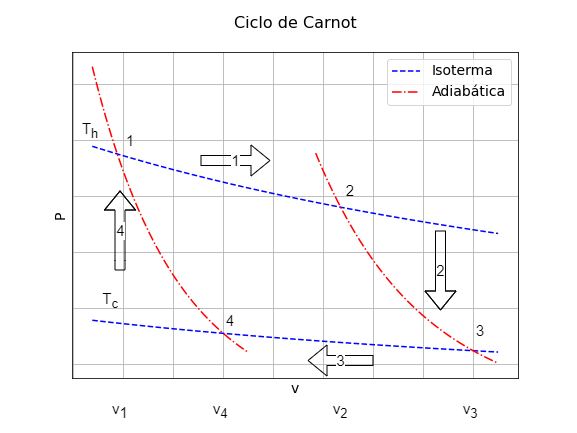
\includegraphics[width=\textwidth]{img/ciclos/ciclo_carnot_final.png}
        \end{figure}
    
            \subsubsubsection{Corolario 1}
            
            \begin{quote}
                \textit{\say{El rendimiento térmico de un ciclo de potencia irreversible es siempre menor que el rendimiento térmico de un ciclo de potencia reversible, cuando ambos operan entre las mismas dos fuentes térmicas.}}
            \end{quote}
            
            \subsubsubsection{Corolario 2}
            
            \begin{quote}
                \textit{\say{Todos los ciclos de potencia reversibles que operan entre las dos mismas fuentes térmicas tienen el mismo rendimiento.}}
            \end{quote}
        
        \end{multicols}
            
        \subsubsection{Ciclo de Carnot}
        
        Etapas reversibles (\textbf{Figura \ref{fig:carnot}}):
        
        \begin{enumerate}
            \item \textbf{Etapa 1}: Expansión Isotérmica:
                \[T_{h}=cte \Rightarrow \Delta U = 0\]
                \[Q_{12}=W_{12}=RT_{h} \ln(\frac{v_{2}}{v_{1}})>0\]
            \item \textbf{Etapa 2}: Expansión Adiabática:
                \[Q_{23}=0 \Rightarrow W_{23}=-\Delta U=-\overline{C_{V}}(T_{c}-T_{h})>0\]
            \item \textbf{Etapa 3}: Compresión Isotérmica:
                \[T_{c}=cte \Rightarrow \Delta U = 0\]
                \[Q_{34}=W_{34}=RT_{c} \ln(\frac{v_{4}}{v_{3}})<0\]
            \item \textbf{Etapa 4}: Compresión Adiabática:
                \[Q_{41}=0 \Rightarrow W_{41}=-\Delta U=-\overline{C_{V}}(T_{h}-T_{c})<0\]
        \end{enumerate}
        
        En general \(C_{v_{23}} \neq C_{v_{41}}\), ya que los \(v\) son distintos en ambos procesos, pera para un \textbf{gas ideal} \(C_{v}\) es independiente de \(v\).
        
        Trabajo neto:
        \[W_{neto}=\sum W_{i}=W_{12}+W_{23}+W_{34}+W_{41}\]
        \[\overset{W_{23}+W_{41}=0}{\Rightarrow} W_{neto}=RT_{h} \ln(\frac{v_{2}}{v_{1}})+RT_{c} \ln(\frac{v_{4}}{v_{3}})\]
        \[\text{Además, }Q_{2}=0 \wedge Q_{4}=0 \text{ procesos adiabáticos, }Q_{3}<0\text{ calor cedido y }Q_{1}>0\text{ calor absorbido}\]
        \[\Rightarrow Q_{abs}=Q_{12}=RT_{h} \ln(\frac{v_{2}}{v_{1}})\]
        \[\eta = \frac{W_{neto}}{Q_{abs}}\]
        \begin{equation}
        \label{primer_eta}
            \eta_{Carnot} = \left ( \frac{W_{neto}}{Q_{abs}} \right )_{Carnot}=\frac{RT_{h} \ln(\frac{v_{2}}{v_{1}})+RT_{c} \ln(\frac{v_{4}}{v_{3}})}{RT_{h} \ln(\frac{v_{2}}{v_{1}})}
        \end{equation}
        
        Considerando las etapas adiabáticas:
        \[Tv^{\gamma -1}=cte\]
        \[T_{h}{v_{1}}^{\gamma -1}=T_{c}{v_{4}}^{\gamma -1} \wedge T_{h}{v_{2}}^{\gamma -1}=T_{c}{v_{3}}^{\gamma -1}\]
        \[\overset{\frac{T_{h}}{T_{c}}=}{\Rightarrow} \left ( \frac{v_{4}}{v_{1}} \right )^{\gamma -1}=\left ( \frac{v_{3}}{v_{2}} \right )^{\gamma -1}\]
        \begin{equation}
        \label{carnot_adiabatico}
            \Rightarrow \ln(\frac{v_{2}}{v_{1}}) = \ln(\frac{v_{3}}{v_{4}})
        \end{equation}
        
        Usando la \textbf{Ecuación \ref{carnot_adiabatico}} en la \textbf{Ecuación \ref{primer_eta}}:
        \[\eta_{Carnot}=\frac{\not{R}(T_{h}-T_{c}) \not{\ln(\frac{v_{2}}{v_{1}})}}{\not{R}T_{h}\not{\ln(\frac{v_{2}}{v_{1}})}}=\frac{T_{h}-T_{c}}{T_{h}}\]
        \begin{equation}
        \label{eficiencia_carnot}
            \eta_{Carnot}=1-\frac{T_{c}}{T_{h}}
        \end{equation}
        
        De la \textbf{Ecuación \ref{eficiencia_carnot}} se tiene:
        
        \begin{quote}
            \textit{\say{La eficiencia térmica del Ciclo de Carnot depende exclusivamente de las temperaturas extremas, siendo independiente de la naturaleza del sistema}}
        \end{quote}
        
    \subsection{Definición Entropía}
    
    Del Ciclo de Carnot, el trabajo neto también puede ser:
    \[W_{neto}=Q_{absorbido}-|Q_{cedido}|\]
    \[\eta_{Carnot}=\frac{Q_{abs}-|Q_{ced}|}{Q_{abs}}\overset{\text{\textbf{Ecuación \ref{eficiencia_carnot}}}}{=}1-\frac{T_{c}}{T_{h}}\]
    \[1-\frac{T_{c}}{T_{h}}=1-\frac{|Q_{ced}|}{Q_{abs}}\]
    \[\Rightarrow \frac{Q_{abs}}{T_{h}}=\frac{|Q_{ced}|}{T_{c}}\]
    \begin{equation}
    \label{entropia_carnot}
        \sum_{i} \left ( \frac{Q}{T} \right ) = 0
    \end{equation}
    
        \subsubsection{Desigualdad de Clausius}
        
        R. Clausius (1865) definió la Entropía:
        \begin{equation}
        \label{clausius_entropia}
            dS=\frac{\delta q_{reversible}}{T}
        \end{equation}
        
        Para un proceso reversible en un sistema cerrada (usando la definición en la \textbf{Ecuación \ref{clausius_entropia}}):
        \begin{equation}
        \label{definicion_entropia}
            \Delta S=S_{2}-S_{1}=\int_{1}^{2} \left ( \frac{\delta q}{T} \right )_{rev}
        \end{equation}
        
        Y propuso para un \textbf{proceso cíclico}, lo que se conoce como la \textbf{Desigualdad de Clausius}:
        \begin{equation}
        \label{desigualdad_clausius}
            \oint \frac{\delta q}{T} \leq 0
        \end{equation}
        
        \subsubsection{Principio de Incremento de Entropía}
        
        Sea un proceso que ocurre entre los estados \(1\) y \(2\). Sea el camino \(1\rightarrow2\) reverseible o irreversible y el camino \(2\rightarrow1\) reversible. Usando la desigualdad (\textbf{Ecuación \ref{desigualdad_clausius}}):
        \[\oint \frac{\delta q}{T}=\int_{1}^{2} \frac{\delta q}{T}+\int_{2}^{1} \left ( \frac{\delta q}{T} \right )_{rev}=\int_{1}^{2} \frac{\delta q}{T}-\int_{1}^{2} \left ( \frac{\delta q}{T} \right )_{rev} \leq 0\]
        \[\Rightarrow \int_{1}^{2} \frac{\delta q}{T} \leq \int_{1}^{2} \left ( \frac{\delta q}{T} \right )_{rev}\]
        \[\overset{\text{\textbf{Ecuación \ref{definicion_entropia}}}}{\Rightarrow} \Delta S=(S_{2}-S_{1}) \geq \int_{1}^{2} \frac{\delta q}{T}\]
        
        \begin{quote}
            \textit{\say{El cambio de entropía de un sistema cerrado es (1) mayor que la integral \(\int_{1}^{2} \frac{\delta q}{T}\) para un proceso irreversible y (2) igual a la integral \(\int_{1}^{2} \frac{\delta q}{T}\) para un proceso reversible.}}
        \end{quote}
        
        En consecuencia,
        \begin{equation}
        \label{principio_entropia}
            \Delta S_{\text{(Sistema Cerrado)}} \geq 0
        \end{equation}
        
        En resumen:
        
        \begin{quote}
            \textit{\say{La Entropía es una propiedad que no se conserva. Los procesos naturales se mueven en la dirección del aumento entrópico del Universo, que es el mayor sistema aislado en que estamos inmersos.}}
        \end{quote}
        \begin{quote}
            \textit{\say{El desempeño de los sistemas de ingeniería se degrada por la presencia de irreversibilidades y la generación de entropía es una medida de la magnitud de las irreversibilidades presentes durante un proceso.}}
        \end{quote}
        
    \subsection{Medición de Entropía: Relaciones de Maxwell}
    
    Usando la Primera Ley (\textbf{Ecuación \ref{def_energia}}), la definición de trabajo (\textbf{Ecuación \ref{def_trabajo}}) y la definición de Entropía (o Segunda Ley) (\textbf{Ecuación \ref{clausius_entropia}}):
    \[dE=q-w \overset{\text{\textbf{Ecuación \ref{clausius_entropia}}}}{\Rightarrow}q=TdS \overset{\text{\textbf{Ecuación \ref{def_trabajo}}}}{\Rightarrow} w=Pdv\]
    \begin{equation}
    \label{ec_fund_energia}
        dE = TdS - Pdv
    \end{equation}
    Que se conoce como la \textbf{Ecuación Fundamental de Energía}, pues es expresada sólo en función de variables de estado. De forma análoga se obtiene (recordando la \textbf{Ecuación \ref{entalpia}}):
    \[H = E + Pv\]
    \[\overset{\text{Versión derivada}}{\Rightarrow} dH = d(E+ Pv)=dE + d(Pv)=dE + Pdv + vdP\]
    \[\overset{\text{\textbf{Ecuación \ref{ec_fund_energia}}}}{\Rightarrow} dH=(TdS-Pdv)+Pdv + vdP\]
    \begin{equation}
    \label{ec_fund_entalpia}
        dH=TdS+vdP
    \end{equation}
    Si consideramos: \(S=f(v,T)\) y \(S=f(P,T)\):
    \[dS=\left ( \frac{\partial S}{\partial v} \right )_{T}dv+\left ( \frac{\partial S}{\partial T} \right )_{v}dT \wedge dS=\left ( \frac{\partial S}{\partial P} \right )_{T}dP+\left ( \frac{\partial S}{\partial T} \right )_{P}dT\]
    Buscando los coeficientes \(\left ( \frac{\partial S}{\partial i} \right )_{j}\text{, con }i \neq j=v,P,T\):
    \[\overset{\text{Desde \textbf{Ecuación \ref{ec_fund_energia}}}}{\Rightarrow}\left ( \frac{\partial E}{\partial S} \right )_{v}=\left ( \frac{\partial (TdS-Pdv)}{\partial S} \right )_{v}=T\Rightarrow \left ( \frac{\partial E}{\partial T} \right )_{v}\left ( \frac{\partial T}{\partial S} \right )_{v}=T\]
    \[\overset{\text{Usando \textbf{Ecuación \ref{ley_de_joule}}}}{\Rightarrow}C_{v}\left ( \frac{\partial T}{\partial S} \right )_{v}=T\Rightarrow \left \| \left ( \frac{\partial S}{\partial T} \right )_{v}=\frac{C_{v}}{T} \right \|\]
    \[\overset{\text{Desde \textbf{Ecuación \ref{ec_fund_entalpia}}}}{\Rightarrow}\left ( \frac{\partial H}{\partial S} \right )_{P}=\left ( \frac{\partial (TdS+vdP)}{\partial S} \right )_{P}=T\Rightarrow \left ( \frac{\partial H}{\partial T} \right )_{P}\left ( \frac{\partial T}{\partial S} \right )_{P}=T\]
    \[\overset{\text{Usando \textbf{Ecuación \ref{entalpia_cp}}}}{\Rightarrow}C_{P}\left ( \frac{\partial T}{\partial S} \right )_{P}=T\Rightarrow \left \| \left ( \frac{\partial S}{\partial T} \right )_{P}=\frac{C_{P}}{T} \right \|\]
    \[\overset{\text{Desde \textbf{Ecuación \ref{ec_fund_energia}}}}{\Rightarrow}\left ( \frac{\partial E}{\partial v} \right )_{T}=\left ( \frac{\partial (TdS-Pdv)}{\partial v} \right )_{T}=T\left ( \frac{\partial S}{\partial v} \right )_{T}-P\;/\left . \frac{\partial}{\partial T} \right |_{v}\]
    \begin{equation}
    \label{eq_step_1}
        \Rightarrow \left ( \frac{\partial^{2}E}{\partial v \partial T}\right )_{v}=1\cdot \left ( \frac{\partial S}{\partial v} \right )_{T} + T\left ( \frac{\partial^{2}S}{\partial v \partial T} \right )_{v} - \left ( \frac{\partial P}{\partial T} \right )_{v}
    \end{equation}
    \begin{equation}
    \label{eq_step_2}
        \overset{\text{Como}}{\Rightarrow} \left ( \frac{\partial E}{\partial T} \right )_{v}=T \left ( \frac{\partial S}{\partial T} \right )_{v}\overset{\left . \frac{\partial}{\partial v} \right |_{T}}{\Rightarrow} \left ( \frac{\partial^{2} E}{\partial T \partial v} \right )_{T}=T \left ( \frac{\partial^{2} S}{\partial T \partial v} \right )_{T}
    \end{equation}
    
    \[\overset{\text{Usando \textbf{Ecuación \ref{eq_step_2}} en \textbf{Ecuación \ref{eq_step_1}}}}{\Rightarrow} \left \| \left ( \frac{\partial S}{\partial v} \right )_{T}=\left ( \frac{\partial P}{\partial T} \right )_{v} \right \|\]
    
    \[\overset{\text{Desde \textbf{Ecuación \ref{ec_fund_entalpia}}}}{\Rightarrow} \left( \frac{\partial H}{\partial P} \right )_{T}=\left( \frac{\partial (TdS+vdP)}{\partial P} \right )_{T}=T\left ( \frac{\partial S}{\partial P} \right )_{T}+v\]
    
    \begin{equation}
    \label{eq_step_3}
        \overset{\left . \frac{\partial}{\partial T} \right |_{P}}{\Rightarrow} \left ( \frac{\partial^{2}H}{\partial P \partial T} \right )_{P} = \left ( \frac{\partial S}{\partial P} \right )_{T}+T\left ( \frac{\partial^{2} S}{\partial T \partial P} \right )_{P}+\left ( \frac{\partial v}{\partial T} \right )_{P}
    \end{equation}
    \begin{equation}
    \label{eq_step_4}
        \overset{\text{Como}}{\Rightarrow} \left ( \frac{\partial H}{\partial T} \right )_{P}=T \left ( \frac{\partial S}{\partial T} \right )_{P}\overset{\left . \frac{\partial}{\partial T} \right |_{P}}{\Rightarrow} \left ( \frac{\partial^{2} H}{\partial T \partial P} \right )_{P}=T \left ( \frac{\partial^{2} S}{\partial T \partial P} \right )_{P}
    \end{equation}
    \[\overset{\text{Usando \textbf{Ecuación \ref{eq_step_4}} en \textbf{Ecuación \ref{eq_step_3}}}}{\Rightarrow} \left \| \left ( \frac{\partial S}{\partial P} \right )_{T}=-\left ( \frac{\partial v}{\partial T} \right )_{P} \right \|\]
    \newpage
    
    \textbf{Relaciones de Maxwell}:
    \begin{multicols}{2}
        \begin{equation}
        \label{maxwel_1}
            \left ( \frac{\partial S}{\partial T} \right )_{v}=\frac{C_{v}}{T}
        \end{equation}
        \begin{equation}
        \label{maxwel_2}
            \left ( \frac{\partial S}{\partial T} \right )_{P}=\frac{C_{P}}{T}
        \end{equation}
        
        \begin{equation}
        \label{maxwel_3}
            \left ( \frac{\partial S}{\partial v} \right )_{T}=\left ( \frac{\partial P}{\partial T} \right )_{v}
        \end{equation}
        \begin{equation}
        \label{maxwel_4}
            \left ( \frac{\partial S}{\partial P} \right )_{T}=-\left ( \frac{\partial v}{\partial T} \right )_{P}
        \end{equation}
    \end{multicols}
    Con lo cual:
    \begin{equation}
    \label{delta_entropia}
        dS=\frac{C_{v}}{T}dT+\left ( \frac{\partial P}{\partial T} \right )_{v}dv \wedge dS=\frac{C_{P}}{T}dT-\left ( \frac{\partial v}{\partial T} \right )_{P}dP
    \end{equation}
    \begin{quote}
        \textit{\say{Ecuaciones válidas para cualquier proceso, con la única restricción que sea \textbf{reversible}.}}
    \end{quote}
    \textit{Ejemplo}: Gas ideal:
    \begin{equation}
    \label{gas_ideal_entropia}
        \Delta S^{*}=\overline{C_{v}}\ln(\frac{T_{2}}{T_{1}})+R\ln(\frac{v_{2}}{v_{1}}) \wedge \Delta S^{*}=\overline{C_{P}}\ln(\frac{T_{2}}{T_{1}})-R\ln(\frac{P_{2}}{P_{1}})
    \end{equation}

\section{Tercera Ley de la Termodinámica: Cero absoluto}

\[\text{Cristal Puro} \rightarrow T=0[K] \rightarrow S=0\]

\begin{quote}
    \textit{\say{La entropía de una sustancia pura cristalina con una temperatura absoluta de cero es cero \textbf{pues no hay incertidumbre sobre el estado de las moléculas en ese momento}.}}
\end{quote}

\section{Termoquímica}

    \subsection{Nociones Básicas}
    
    Para mantener estable una reacción de combustión:
    
    \begin{multicols}{3}
    \begin{enumerate}
        \item Combustible.
        \item Oxidante (\(O_{2}\)).
        \item Calor.
    \end{enumerate}
    \end{multicols}
    
    \subsection{Entalpías de Formación}
    
    \begin{equation}
    \label{entalpia_formacion}
        h_{i}(T)=h_{(f,i)}(T_{ref})+\int_{T_{ref}}^{T}c_{(p,i)}dT \text{, con }h_{(f,i)}= \text{ entalía de formación}
    \end{equation}
    
    \begin{quote}
        \textit{\say{Las entalpías de formación, se consideran cero para las sustancias que se encuentra en sus estado natural.}}
    \end{quote}
    
    \subsection{Combustión}
    
    \begin{quote}
        \textit{\say{\textbf{Primer principio}: Variación de energía debida a la variación del calor liberado y al trabajo realizado por un sistema.}}
    \end{quote}
    
    \begin{quote}
        \textit{\say{La combustión tiene lugar siempre en fase gaseosa. Líquidos se evaporan antes, y sólidos se subliman y se descomponen (\textbf{pirólisis})}}
    \end{quote}
    
    Considerando el primer principio (\textbf{Ecuación \ref{def_energia}}):
    
    \[\delta q = dE + Pdv\]
    \[\overset{P=cte}{\Rightarrow} dH=\delta q\]
    \[\overset{\int}{\Rightarrow} Q = H_{P} - H_{R} \text{, con }P= \text{producto y }R= \text{reactante}\]
    
    Calor liberado:
    
    \begin{equation}
    \label{entalpia_liberada}
        \Delta H_{rxn} = \sum_{i} v_{i}H_{i} \text{, con }v_{i}= \text{coeficientes estequiométricos}
    \end{equation}
    
    Con la convención:
    
    \[\begin{matrix}
        v_{i} > 0 &  & \text{productos}\\ 
        v_{i} < 0 &  & \text{reactantes}
    \end{matrix}\]
    
    Efecto de la temperatura. Derivando la \textbf{Ecuación \ref{entalpia_liberada}}:
    
    \[\left ( \frac{\partial \Delta H_{rxn}}{\partial T} \right )_{P} = \sum_{i}v_{i} \left ( \frac{\partial H_{i}}{\partial T} \right )_{P} \overset{\text{Ecuación \ref{entalpia_cp}}}{=} \sum_{i}v_{i}C_{(P, i)}\]
    \[\overset{dT}{\Rightarrow} \left ( \frac{\partial \Delta H_{rxn}}{\partial T} \right )_{P} dT = \left ( \sum_{i}v_{i}C_{(P, i)} \right ) dT\]
    \[\Rightarrow \int_{T_{0}=298[K]}^{T=T} (\;)\]
    \begin{equation}
    \label{entalpia_temp}
        \left ( \Delta H_{rxn}\right )_{T} - \left ( \Delta H_{rxn} \right )_{T_{0}=298[K]\approx 25[{}^{o}C]} = \int_{T_{0}}^{T} \left ( \sum_{i} v_{i} C_{(P, i)} \right ) dT
    \end{equation}
    
    \subsection{Cambio de Fase: Calor latente de Evaporación}
    
    Ejemplo: Combustión de Metano (\(CH_{4}\)) (\textbf{Figura \ref{fig:com_met}})
    
    \[\begin{matrix}
        {CH_{4}}_{(g)} + 2{O_{2}}_{(g)} = {CO_{2}}_{(g)} + 2{H_{2}O}_{(l)} &  & \Delta H_{comb}=-212.8 \left [ \frac{kcal}{mol} \right ]
    \end{matrix}\]
    
    \begin{multicols}{2}
        \begin{figure}[H]
            \caption{Combustión de \(CH_{4}\)}
            \label{fig:com_met}
            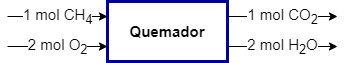
\includegraphics[width=\textwidth]{img/esquemas/combustion_metano.png}
        \end{figure}
        
        Como el producto es \(H_{2}O\) \textbf{líquido}, el valor se denomina \textbf{Poder Calorífico Superior}. Experimentalmente, el agua se evapora. Al agregar este calor extra, el valor se denomina \textbf{Poder Calorífico Inferior}.
    \end{multicols}
    
    \[\begin{matrix}
        \begin{matrix}
            {CH_{4}}_{(g)} + 2{O_{2}}_{(g)} & = & {CO_{2}}_{(g)} + 2{H_{2}O}_{(l)} &  & \Delta H_{comb}=-212.8 \left [ \frac{kcal}{mol} \right ] \\ 
            {H_{2}O}_{(l)} & = & {H_{2}O}_{(g)} &  & \Delta H_{vap}=+10.514 \left [ \frac{kcal}{mol} \right ]\\
        \end{matrix} \\
        \overline{\begin{matrix}
            {CH_{4}}_{(g)} + 2{O_{2}}_{(g)} & = & {CO_{2}}_{(g)} + 2{H_{2}O}_{(g)} &  & \Delta H_{comb}=-191.8 \left [ \frac{kcal}{mol} \right ]
        \end{matrix}}
    \end{matrix}\]
    
    \subsection{Temperatura de llama adiabática}
    
    \begin{multicols}{2}
        Aplicando condiciones adiabáticas, no hay pérdidas de calor al ambiente.
        
        \[\Delta H_{calentamiento} = -\Delta H_{rxn}\]
        
        \[\overset{\text{Ecuación \ref{entalpia_temp}}}{\Rightarrow} \Delta H_ {calentamiento}= \int_{T_{0}}^{T} \left ( \sum_{i}v_{i}C_{(P, i)} \right )_{productos} dT\]
        
        \begin{figure}[H]
            \caption{Reacción adiabática de una llama}
            \label{fig:com_llama}
            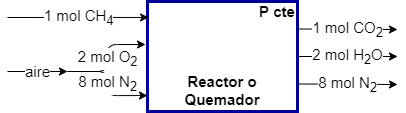
\includegraphics[width=\textwidth]{img/esquemas/llama_adiabatica.png}
        \end{figure}
    \end{multicols}
    
    \[\left ( \sum_{i}v_{i}C_{(P, i)} \right )_{productos} = 1\cdot C_{(P, CO_{2})} + 2\cdot C_{(P, H_{2}O)} + 8\cdot C_{(P, N_{2})}\]
    
    Para \(C_{(P, i)}\) molar usamos la función cuadrática (\textbf{Ecuación \ref{cp_cuadratica}}):
    
    \[C_{(P, i)}(T)=\alpha_{i} + \beta_{i}T + \gamma_{i}T^{2}\]
    
    \[\begin{matrix}
        \overset{\text{Aplicando para los gases}}{\Rightarrow} 1\cdot C_{(P, CO_{2})} + 2\cdot C_{(P, H_{2}O)} + 8\cdot C_{(P, N_{2})} = & 1\cdot (\alpha_{CO_{2}} + \beta_{CO_{2}}T + \gamma_{CO_{2}}T^{2}) + \\
        & 2\cdot(\alpha_{H_{2}O} + \beta_{H_{2}O}T + \gamma_{H_{2}O}T^{2}) + \\
        & 8\cdot(\alpha_{N_{2}} + \beta_{N_{2}}T + \gamma_{N_{2}}T^{2})
    \end{matrix}\]
    \[=(1\cdot\alpha_{CO_{2}} + 2\cdot\alpha_{H_{2}O} + 8\cdot\alpha_{N_{2}}) + (1\cdot\beta_{CO_{2}} + 2\cdot\beta_{H_{2}O} + 8\cdot\beta_{N_{2}})T 
    + (1\cdot\gamma_{CO_{2}} + 2\cdot\gamma_{H_{2}O} + 8\cdot\gamma_{N_{2}})T^{2}\]
    \[\overset{\text{Definiendo}}{\equiv} \alpha_{productos} + \beta_{productos}T + \gamma_{productos}T^{2}\]
    \[\left ( \sum_{i}v_{i}C_{(P, i)} \right )_{productos} = \alpha_{productos} + \beta_{productos}T + \gamma_{productos}T^{2}\]
    \[\overset{\text{Reemplazando}}{\Rightarrow} \int_{T_{0}}^{T} (\alpha_{productos} + \beta_{productos}T + \gamma_{productos}T^{2}) dT = -\Delta H_{rxn}\]
    \[\Rightarrow \alpha_{producto}(T - T_{0}) + \frac{\beta_{producto}}{2}(T^{2} - T_{0}^{2}) + \frac{\gamma_{producto}}{3}(T^{3} - T_{0}^{3})=-\Delta H_{rxn}\]
    \[\alpha_{producto}T+\frac{\beta_{producto}}{2}T^{2} + \frac{\gamma_{producto}}{3}T^{3} = -\Delta H_{rxn} - \alpha_{producto}T_{0}-\frac{\beta_{producto}}{2}T_{0}^{2} - \frac{\gamma_{producto}}{3}T_{0}^{3}\]
    
    \begin{multicols}{2}
        Reemplazando los valores de \(\Delta H_{rxn}\), \(\alpha_{producto}\), \(\beta_{producto}\), \(\gamma_{producto}\) y \(T_{0}=298[K]\). La solución a la ecuación cúbica anterior es, aproximadamente:
        \[T\approx2238[K]\approx1965[{}^{o}C]\]
        
        Para aumentar esta temperatura se puede (1) eliminar el inerte \(N_{2}\) o (2) precalentar los gases reaccionantes.
        
        Se asume \(100\%\) de conversión de combustible. Considerando el caso general:
        \[C_{m}H_{n}+\left ( m + \frac{n}{4} \right )O_{2}=mCO_{2}+\frac{n}{2}H_{2}O\]
        
        \begin{figure}{H}
            \caption{Esquema de una llama (Fuente: Clase 6)}
            \label{fig:llama}
            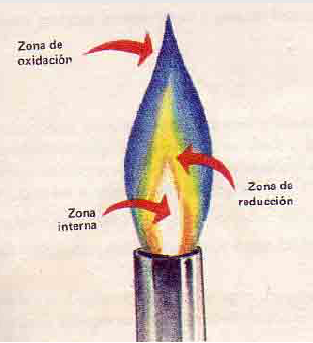
\includegraphics[width=.9\textwidth]{img/clases/llama.png}
        \end{figure}
    \end{multicols}
    
    \begin{figure}[H]
        \centering
        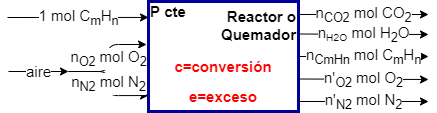
\includegraphics[width=.8\textwidth]{img/esquemas/llama_no_adiabatica.png}
        \caption{Reacción no adiabática de una llama}
        \label{fig:com_no_llama}
    \end{figure}
    
    Para la \textbf{Figura \ref{fig:com_no_llama}} se tiene que:
    
    \[\Delta H_{calentamiento}=-c(\Delta H_{rxn})\]
    \[n_{O_{2}}=(1+e)\left ( m + \frac{n}{4} \right )\text{, moles de entrada de }O_{2}\]
    \[n_{N_{2}}=4(1+e)\left ( m + \frac{n}{4} \right )\text{, moles de entrada de }N_{2}\]
    \[n_{CO_{2}}=mc\text{, moles de salida de }CO_{2}\]
    \[n_{H_{2}O}=c \frac{n}{2}\text{, moles de salida de }H_{2}O\]
    \[n_{C_{m}H_{n}}=1-c\text{, moles de salida de }C_{m}H_{n}\]
    \[n_{O_{2}}^{'}=(1-c+e)\left ( m + \frac{n}{4} \right )\text{, moles de salida de }O_{2}\]
    \[n_{N_{2}}^{'}=4(1+e)\left ( m + \frac{n}{4} \right )\text{, moles de salida de }N_{2}\]
    
    \subsection{Balance de energía}
    
    Viendo esto como \textbf{Procesos de Flujo}:
    
    \begin{quote}
        \textit{\say{Siempre consideramos estado estacionario.}}
    \end{quote}
    
    \[E_{entrada}=E_{salida}\]
    \[\text{Usando la notación } \dot{f}\equiv \frac{\partial f}{\partial t},\;h_{T_{0}}=h^{0}\]
    \[\dot{Q_{ent}}+\dot{W_{ent}}+\sum_{i} \dot{n_{R}}(h_{(f,i)}^{o}+h_{i}-h_{i}^{o})_{R}=\dot{Q_{sal}}+\dot{W_{sal}}+\sum_{i} \dot{n_{P}}(h_{(f,i)}^{o}+h_{i}-h_{i}^{o})_{P}\]
    \begin{equation}
    \label{balance_proc_flujo}
        \dot{Q_{ent}}+\dot{W_{ent}}+H_{R}=\dot{Q_{sal}}+\dot{W_{sal}}+H_{P}
    \end{equation}
    
        \subsubsection{Sistema Cerrado}
        
        \[(Q_{ent}-Q_{sal})+(W_{ent}-W_{sal})=U_{productos}-U_{reactantes} \Rightarrow\]
        
        \begin{equation}
        \label{sis_cerrado_termoquimica}
            Q-W=\sum_{i} \dot{n_{P}}(h_{(f,i)}^{o}+h_{i}-h_{i}^{o}-Pv)_{P} - \sum_{i} \dot{n_{R}}(h_{(f,i)}^{o}+h_{i}-h_{i}^{o}-Pv)_{R}
        \end{equation}
        
        \subsubsection{Balance de Calor}
        
        \begin{quote}
            \textit{\say{Flujo molar de los gases \(\cdot\) la suma de Calor de reacción \(+\) Calor para calentar los productos, es igual (\(=\)) al Flujo de calor para calentar el vapor.}}
        \end{quote}
        
        \begin{equation}
        \label{balance_calor_termpoquimica}
            \dot{n}\cdot (Q_{rxn}+Q_{calent}) = \dot{Q_{vapor}}
        \end{equation}
        
\section{Procesos de Flujo}

\begin{quote}
    \textit{\say{Sistema abierto, proceso de flujo, hay intercambio de masa y energía.}}
\end{quote}
    
    \subsection{Principio de Conservación de Materia}
    
    \begin{multicols}{2}
    \begin{figure}[H]
        \centering
        \label{fig:control_vol}
        \caption{Volumen de Control (Fuente: Clase 7)}
        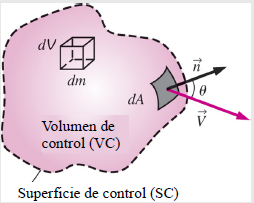
\includegraphics[width=.85\textwidth]{img/clases/volumen_control.png}
    \end{figure}

    \[\begin{matrix}
        \begin{matrix}
            & \text{Entrada a volumen de control en }\Delta t \\
            - & \text{ Salida de volumen de control en }\Delta t
        \end{matrix} \\
        \overline{\text{ Cambio \textbf{neto} en volumen de control durante }\Delta t}
    \end{matrix}\]
    
    \[\frac{dm_{e}}{dt} - \frac{dm_{s}}{dt} = \frac{d}{dt}m_{VC}\]
    
    \[\overset{\frac{df}{dt}\equiv \dot{f}}{\Rightarrow} \dot{m_{e}} - \dot{m_{s}} = \frac{d}{dt} \int_{CV} \rho dt\]
    
    \[\sum_{e} \dot{m} - \sum_{s} \dot{m} = \frac{d}{dt} \int_{CV} \rho dt\]
    \end{multicols}
    
    Para un flujo estable y continuo (\textbf{Estado Estacionario}):
    
    \[\frac{d}{dt}=0 \Rightarrow \sum_{e} \dot{m} = \sum_{s} \dot{m}\]

    \subsection{Energía de Flujo}
    
    \begin{quote}
        \textit{\say{Se requiere un trabajo (Trabajo o Energía de Flujo) que empuja la masa hacia y fuera del volumen de control (\(VC\))}. Esto se representa con un \textbf{Pistón Imaginario}}
    \end{quote}
    
    \[W_{\text{pistón imaginario}} = F \cdot l = P \cdot A \cdot l\]
    \begin{equation}
    \label{en_flujo}
        \text{Energía de Flujo} \equiv EF = P \cdot V
    \end{equation}
    \[\overset{\text{En unidades de masa}}{\Rightarrow} EF = Pv\]
    
        \subsubsection{Balance de Energía}
        
        Usando \textbf{Ecuación \ref{def_energia}} a procesos de flujo:
        
        Definiendo:
        \[\text{Energía Cinética} \equiv EC\]
        \[\text{Energía Potencial} \equiv EP\]
        \[\text{Energía Total} \equiv E_{T}\]
        
        Nos queda:
        \begin{equation}
        \label{en_total_flujo}
            dE_{T}=dU+d(EF)+d(EC)+d(EP)=q-w
        \end{equation}
        
        \begin{multicols}{2}
            \begin{figure}[H]
                \caption{Diagrama Pv para un proceso de flujo}
                \label{fig:proc_flujo}
                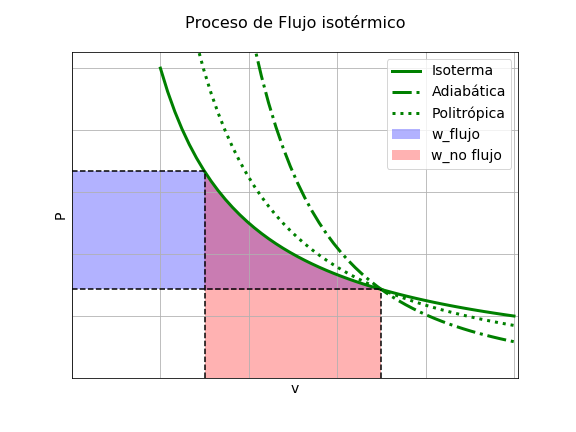
\includegraphics[width=\textwidth]{img/graficos/proc_flujo.png}
            \end{figure}
            
            \[dU+d(Pv)+d(EC)+d(EP)=q-w\]
            \[\overset{\text{\textbf{Ecuación \ref{entalpia}}}}{\Rightarrow} dH+d(EC)+d(EP)=q-w\]
            
            Si los cambios de energía cinética y potencial son pequeñas:
            \[dH=q-w_{flujo}\]
            
            Volviendo desde la definición de Entalpía:
            \[dU + d(Pv) = q - w_{flujo}\]
            \[\Leftrightarrow dU + vdP + Pdv = q - w_{flujo}\]
        \end{multicols}
        
        \[\overset{\text{Procesos reversibles}}{\Rightarrow} \text{\textbf{Ecuación \ref{ec_fund_energia}}, \textbf{Ecuación \ref{clausius_entropia}}} \Rightarrow \not{TdS} - \not{Pdv} + vdP + \not{Pdv} = \not{TdS} - w_{flujo}\]
        \begin{equation}
        \label{trabajo_flujo}
            w_{flujo} = -vdP
        \end{equation}
        
            \subsubsubsection{Proceso Isotérmico}
            
            Usando \textbf{Ecuación \ref{presion_ideal}}, tenemos:
            \[Pv = RT = cte\]
            \[d(Pv) = 0\]
            \[\Leftrightarrow vdP + Pdv = 0\]
            \[\Leftrightarrow Pdv = - vdP\]
            \[\overset{\text{\textbf{Ecuación \ref{trabajo_flujo}}}}{\Rightarrow} w_{\text{no flujo}} = w_{flujo}\]
            
            La curva isotérmica se muestra en la \textbf{Figura \ref{fig:proc_flujo}} como una línea verde continua. La equivalencia de los trabajos se muestra en las áreas coloreadas.
            
            \subsubsubsection{Proceso adiabático}
            
            Usando \textbf{Ecuación \ref{poisson_2}}, tenemos:
            \[Pv^{\gamma} = cte\]
            
            \textbf{Proceso no flujo}:
            
            \[Pdv = \frac{k}{v^{\gamma}}dv\]
            \[\overset{\int}{\Rightarrow} \int_{1}^{2} Pdv = k \int_{1}^{2} v^{-\gamma}dv\]
            \[\begin{matrix}
                \Rightarrow \int_{1}^{2} Pdv & = & \left . k \frac{1}{-\gamma + 1}v^{-\gamma + 1} \right |_{1}^{2} \\
                & = & \left . \frac{1}{1 - \gamma} \left ( \frac{k}{v^{\gamma}} \right ) v \right |_{1}^{2} \\
                & = & \left . \frac{1}{1-\gamma} Pv \right |_{1}^{2}
            \end{matrix}\]
            \begin{equation}
            \label{trabajo_no_flujo_adiab}
                W_{\text{no flujo}} = \frac{1}{1-\gamma}\left ( P_{2}v_{2} - P_{1}v_{1} \right ) = \frac{1}{\gamma - 1}\left ( P_{1}v_{1} - P_{2}v_{2} \right )
            \end{equation}
            
            \textbf{Proceso flujo}
            
            \[-vdP = - \frac{k}{P^{\gamma^{-1}}}dP\]
            \[\overset{\text{Similar a }w_{\text{no flujo}}}{\Rightarrow} \int_{1}^{2} -vdP = \left . \gamma \frac{1}{1-\gamma}vP \right |_{1}^{2}\]
            \begin{equation}
            \label{trabajo_flujo_adiab}
                W_{flujo} = \gamma \frac{1}{1-\gamma} \left ( P_{2}v_{2} - P_{1}v_{1} \right ) = \gamma \frac{1}{\gamma - 1} \left ( P_{1}v_{1} - P_{2}v_{2} \right )
            \end{equation}
            
            Como \(\gamma \geq 1\):
            \[w_{flujo} \geq w_{\text{no flujo}}\]
            
            Lo que se aprecia en la línea discontinua verde de la \textbf{Figura \ref{fig:proc_flujo}}. Si extendemos el área azul (\(w_{flujo}\) hasta la curva adiabática, tendremos la desigualdad de arriba. La curva politrópica se encuentra entre las curvas isotérmica y adiabática.
            
            \subsubsubsection{Resumen}
            
            Teniendo que \(EC = \frac{m\overrightarrow{v}^{2}}{2}\), \(EP = mgz\), \(U = mH\) y \(\Delta E_{T} = 0\) en flujo estacionario:
            
            \[{E_{T}}_{1} = {E_{T}}_{2} \overset{\frac{d}{dt}}{\Rightarrow}\]
            \[\overset{\text{\textbf{Ecuación \ref{en_total_flujo}}}}{\Rightarrow} \dot{Q_{1}} - \dot{W_{1}} + \sum_{1} \dot{m} \left ( H + \frac{\overrightarrow{v}^{2}}{2} + gz \right ) = \dot{Q_{2}} - \dot{W_{2}} + \sum_{2} \dot{m} \left ( H + \frac{\overrightarrow{v}^{2}}{2} + gz \right ) \overset{\dot{Q} = \dot{Q_{1}} - \dot{Q_{2}} \text{ idem } W}{\Rightarrow}\]
            \begin{equation}
            \label{flujo_en_resumen}
                \dot{Q} - \dot{W} = \dot{m} \left ( (H_{2}-H_{1}) + \frac{1}{2}\left ( \overrightarrow{v_{2}}^{2} - \overrightarrow{v_{1}}^{2} \right ) + g(z_{2} - z_{1}) \right )
            \end{equation}
    \newpage
    
    \subsection{Dispositivos}
    
        \subsubsection{Toberas y difusores}
        
        Proceso adiabático \(q=0\), no hay trabajo \(w=0\), \(z_{2} - z_{1}\) se desprecia. Esto en \textbf{Ecuación \ref{flujo_en_resumen}}:
        \[h_{1} + \frac{1}{2}\overrightarrow{v_{1}}^{2} = h_{2} + \frac{1}{2}\overrightarrow{v_{2}}^{2}\]
        
        Para \textbf{Tobera} \(A_{1} > A_{2} \Rightarrow \overrightarrow{v_{1}} \ll \overrightarrow{v_{2}} \wedge P_{1} > P_{2}\).
        
        Para \textbf{Difusor} \(A_{1} < A_{2} \Rightarrow \overrightarrow{v_{1}} \gg \overrightarrow{v_{2}} \wedge P_{1} < P_{2}\).
        
        \subsubsection{Bomba impulsora}
        
        \begin{quote}
            \textit{\say{Dispositivos que aumenta la presión de un fluido que se encuentra en fase líquida consumiendo cierta cantidad de potencia para lograrlo. Generalmente se consideran adiabáticas.}}
        \end{quote}
        
        \subsubsection{Compresores}
        
        \begin{quote}
            \textit{\say{Dispositivos que aumenta la presión de un fluido que se encuentra en fase gaseosa consumiendo cierta cantidad de potencia para lograrlo. Generalmente se consideran adiabáticos y se desprecian los cambios de energía cinética y potencial.}}
        \end{quote}
        
        \subsubsection{Turbina}
        
        \begin{quote}
            \textit{\say{Dispositivos que disminuye la presión de un fluido que se encuentra en fase gaseosa (turbina de vapor o gas) o en fase líquida (turbina hidráulica) produciendo cierta cantidad de potencia. Generalmente se consideran adiabáticas y se pueden despreciar los cambios de energía cinética y potencial, aunque la velocidad de salida es mucho mayor que la de entrada.}}
        \end{quote}
        
        \subsubsection{Cámara de Mezcla}
        
        \begin{quote}
            \textit{\say{Dispositivo en el cual ingresan más de una corriente de fluido (gas ideal o vapor), que luego de mezclarse, salen bajo un mismo estado. La condición de funcionamiento para este equipo, es que las presiones de entrada deben ser iguales a la presión de salida. La cámara de mezcla funciona en régimen permanente y es adiabática.}}
        \end{quote}
        
        \subsubsection{Válvulas de Expansión}
        
        \begin{quote}
            \textit{\say{Dispositivos que estrangula un fluido, sin producir trabajo. Generalmente se consideran adiabáticas y se pueden despreciar los cambios de energía cinética y potencial.}}
        \end{quote}
    
    \subsection{Proceso de Flujo Isoentálpico}
    
    Una válvula estrangulamiento:
    
    \[\Delta H = \overset{\text{Adiabático}}{\not{Q}} - \overset{\text{No se realiza}}{\not{W_{flujo}}} = 0\]
    
        \subsubsection{Coeficiente de Joule-Thompson}
        
        \begin{quote}
            \textit{\say{Variación de la temperatura con respecto a la presión durante un proceso de \textbf{expansión isoentálpica}.}}
        \end{quote}
        
        \begin{equation}
        \label{coef_joule_thompson}
            \mu_{JT} = \left ( \frac{\partial T}{\partial P}\right )_{H}
        \end{equation}
    
        \subsubsection{Curva de Inversión}
        
        \begin{figure}[H]
            \centering
            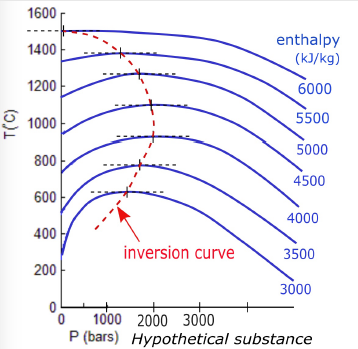
\includegraphics[width=.5\textwidth]{img/clases/curva_inversion.png}
            \caption{Diagrama TP empírico. Cada curva azul es una curva isoentálpica}
            \label{fig:diagrama_t_p}
        \end{figure}
        
        La curva de inversión corresponde a la curva que une los puntos de derivada \(0\).
        
        \begin{equation}
        \label{t_de_inversion}
            \mu_{JT} = 0 \equiv \text{T. de Boyle} \vee \text{T. de Inversión}
        \end{equation}
    \newpage
        
    \subsection{Uso de Tablas de Vapor}
    
    (De un post hecho por Javiera Vergara Z.)
    
    \begin{enumerate}
        \item Si para la presión o temperatura que dan, el valor de la entropía \(S\) o entalpía \(H\) se encuentra entre los valores del líquido saturado y vapor saturados entonces tendremos una mezcla bifásica y un título de vapor, cuyo valor va entre 0 y 1 (0 cuando es liquido saturado y 1 cuando es vapor saturado).
        
        Si el valor de cualquiera de las dos propiedades fuera mayor, entonces, se tratara de \textbf{vapor sobrecalentado}, y por el contrario, si es menor será \textbf{líquido comprimido}.
        
        \item Para calcular el título de vapor:
        \[H = H_{f} + x H_{fg} = x H_{g} + (1 - x) H_{f}\]
        \[S = S_{f} + x S_{fg} = x S_{g} + (1 - x) S_{f}\]
        \[U = U_{f} + x U_{fg} = x U_{g} + (1 - x) U_{f}\]
        
        \item Sobre las fases de un compuestos, tenemos cinco casos:
        
        \begin{figure}[H]
            \centering
            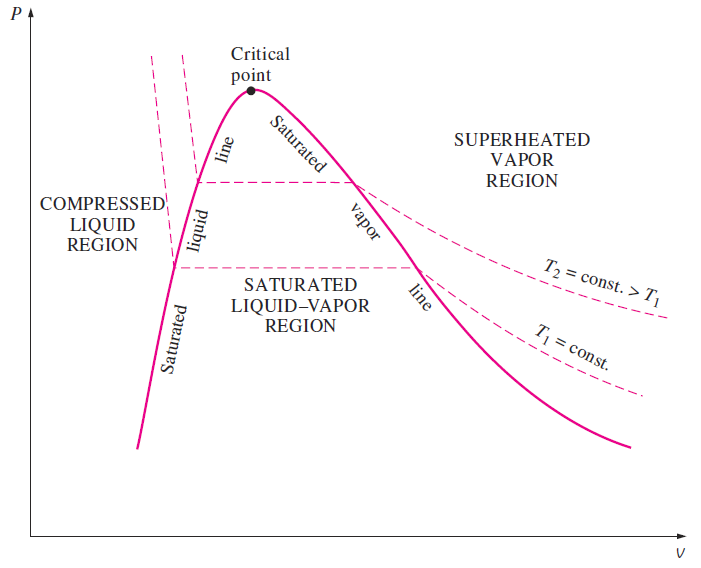
\includegraphics[width=.6\textwidth]{img/clases/diagrama_pv_fases.png}
            \caption{Diagrama Pv para conocer la fase de un compuesto.}
            \label{fig:pv_fases}
        \end{figure}
        
        \begin{multicols}{3}
            \begin{enumerate}
                \item líquido comprimido
                \item líquido saturado
                \item mezcla bifásica
                \item vapor saturado
                \item vapor sobrecalentado
            \end{enumerate}
        \end{multicols}
        
        Todo esto lo podemos ver gráficamente a través de una campana de saturación en un diagrama \textbf{Diagrama Pv} (\textbf{Figura \ref{fig:pv_fases}}).
        
    \end{enumerate}

\section{Ciclos de Potencia}

    \subsection{Ciclo de Carnot}
        
        Ver \textbf{Figura \ref{fig:carnot}}. Eficiencia (\textbf{Ecuación \ref{eficiencia_carnot}}): \(n_{Carnot}=1-\frac{T_{L}}{T_{H}}\)
        
        \begin{enumerate}
            \item Ciclo ideal para una sustancia ideal.
            \item Máquina térmica de rendimiento máximo.
            \item Eficiencia térmica depende exclusivamente de las temperaturas extremas. \textit{Independiente de la naturaleza del sistema}.
        \end{enumerate}

    \subsection{Máquinas de Combustión Interna}

    Recordando, eficiencia de un ciclo de potencia de una máquina biterma (\textbf{Ecuación \ref{ef_biterma}}):
    
    \[\eta = \frac{W_{n}}{Q_{c}} = 1 - \frac{Q_{f}}{Q_{c}} < 1\]
        
        \subsubsection{Ciclos de Gas}
        
        \begin{quote}
            \textit{\say{El fluido de trabajo permanece como gas durante todo el ciclo.}}
        \end{quote}
        
            \subsubsubsection{Máquinas de Combustión Interna}
            
            \begin{figure}[H]
                \caption[Máquinas de combustión interna]{Máquinas de combustión interna: En la realidad la composición del fluido cambia durante el ciclo. Sin embargo, si se considera que en el aire predomina el nitrógeno, este es inerte todo el tiempo. (Fuente: Clase 8)}
                \label{fig:comb_interna}
                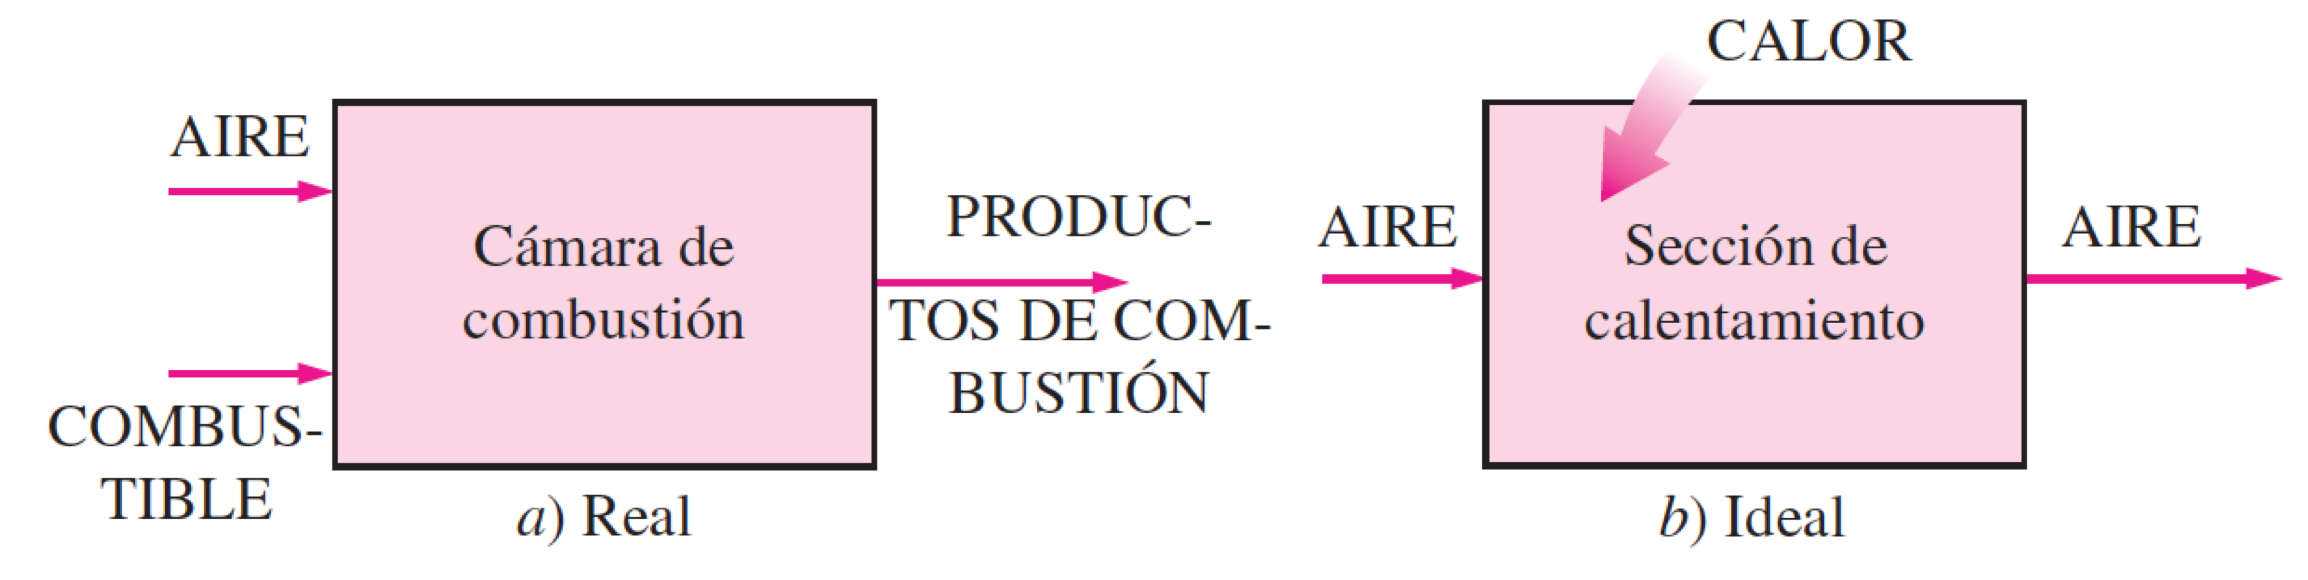
\includegraphics[width=.7\textwidth]{img/clases/combustion_interna.png}
            \end{figure}
            
            \subsubsubsection{Ciclo de Aire Estándar}
            
            \begin{enumerate}
                \item Fluido de trabajo es aire que circula de modo continuo en un circuito cerrado y siempre se comporta como un gas ideal.
                \item Procesos son internamente reversibles.
                \item Combustión se sustituye por adición de calor por fuente externa.
                \item Escape se sustituye por rechazo de calor que regresa al fluido de trabajo a su estado inicial.
            \end{enumerate}
            
        \subsubsection{Motores Alternativos}
            
        \begin{multicols}{2}
            \begin{figure}[H]
            \caption{Motor alternativo (Fuente: Clase 8)}
            \label{fig:motor_alter}
                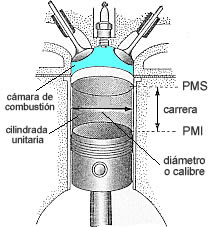
\includegraphics[width=.7\textwidth]{img/clases/motores_alternativos.png}
            \end{figure}
            
            \begin{itemize}
                \item \textbf{Volumen de desplazamiento o cilindrada}: volumen de gas que entra al cilindro. Es el volumen comprendido entre el PMI y el PMS.
                \item \textbf{Volumen de espacio libre}: volumen mínimo al que es comprimido el gas dentro del cilindro.
                \item \textbf{Relación de compresión} del motor (\(r\)):
                \begin{equation}
                \label{rel_comp}
                    r \equiv \frac{v_{max}}{v_{min}} = \frac{v_{\text{PMI}}}{v_{\text{PMS}}}
                \end{equation}
                \vfill \null
                \columnbreak
                
                \item \textbf{PMS}: Punto muerto superior, posición del pistón en el punto máximo de altura.
                \item \textbf{PMI}: Punto muerto inferior, posición más baja del pistón antes de empezar a subir.
                \item \textbf{Carrera (embolada)}: distancia entre el PMS y el PMI. Se expresa en milímetros.
                \item \textbf{Diámetro o calibre}: es el diámetro interior del cilindro y también se expresa en milímetros.
            \end{itemize}
            
            \begin{figure}[H]
            \caption{Motor alternativo, comparando estados del volumen de fluido (Fuente: Clase 8)}
            \label{fig:motor_alter_2}
                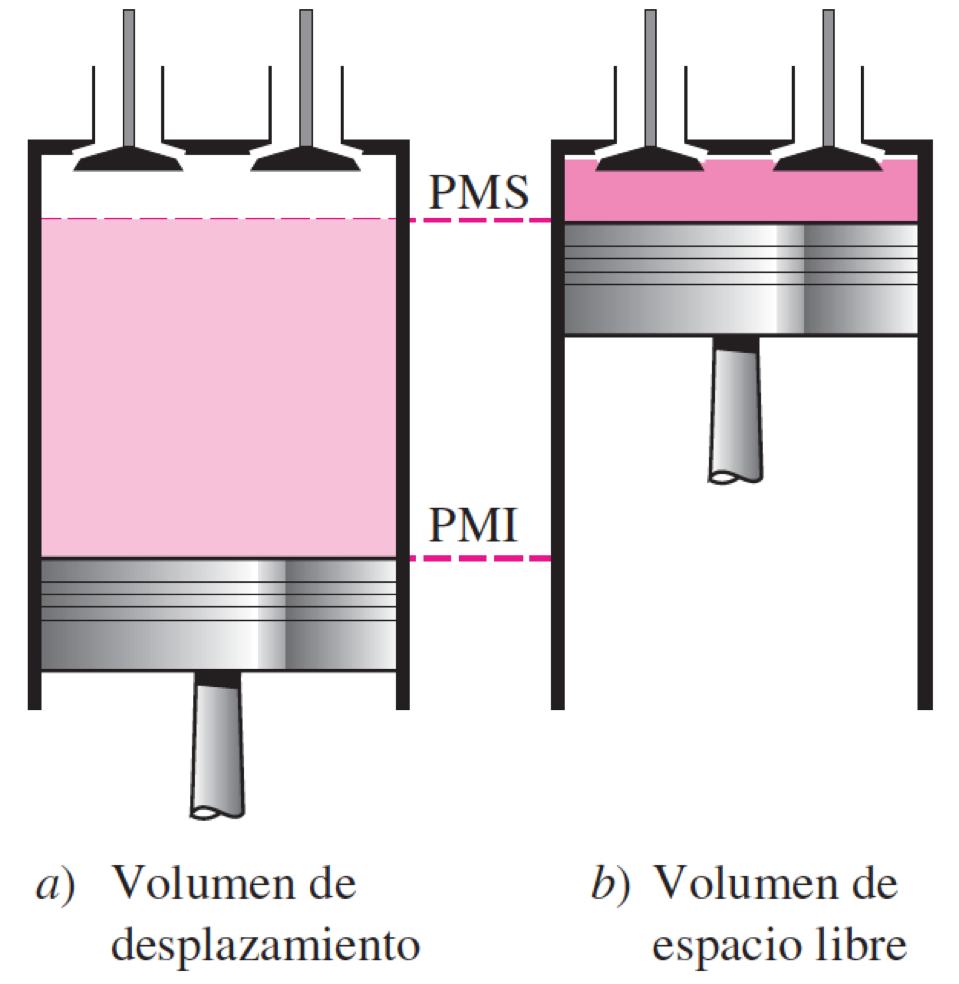
\includegraphics[width=.7\textwidth]{img/clases/motores_alternativos_2.png}
            \end{figure}
        \end{multicols}
        
            \subsubsubsection{Motor de chispa de 4 tiempos}
            
            Admisión \(\rightarrow\) Compresión \(\rightarrow\) Combustión-Expansión \(\rightarrow\) Escape \(\rightarrow\)
        
        \subsubsection{Ciclo de Otto}
        
            \subsubsubsection{Motor Otto}
            
            \begin{figure}[H]
                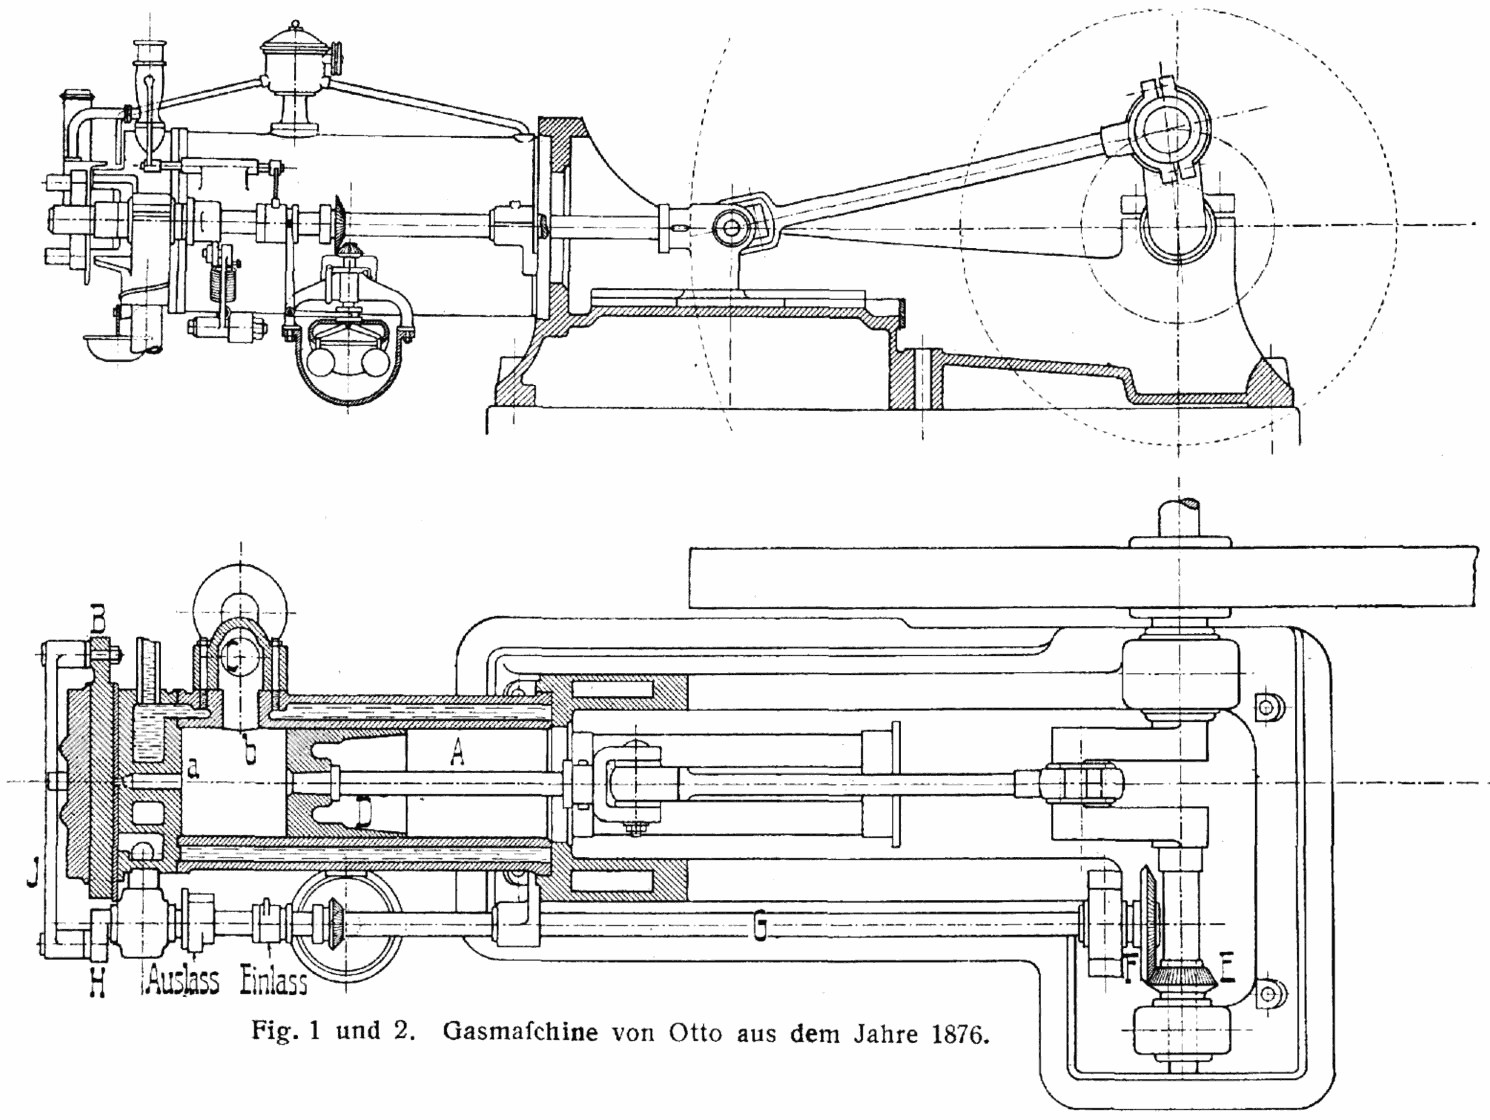
\includegraphics[width=.6\textwidth]{img/clases/motor_otto.png}
                \caption{Motor Otto (Fuente: Clase 8)}
                \label{fig:motor_otto}
            \end{figure}
            
            El motor Otto (\textbf{Figura \ref{fig:motor_otto}}) fue el primer motor de explosión de cuatro tiempos (Nicolaus Otto, 1876).
            
            \subsubsubsection{Ciclo Otto Estándar}
            
            \begin{figure}[H]
                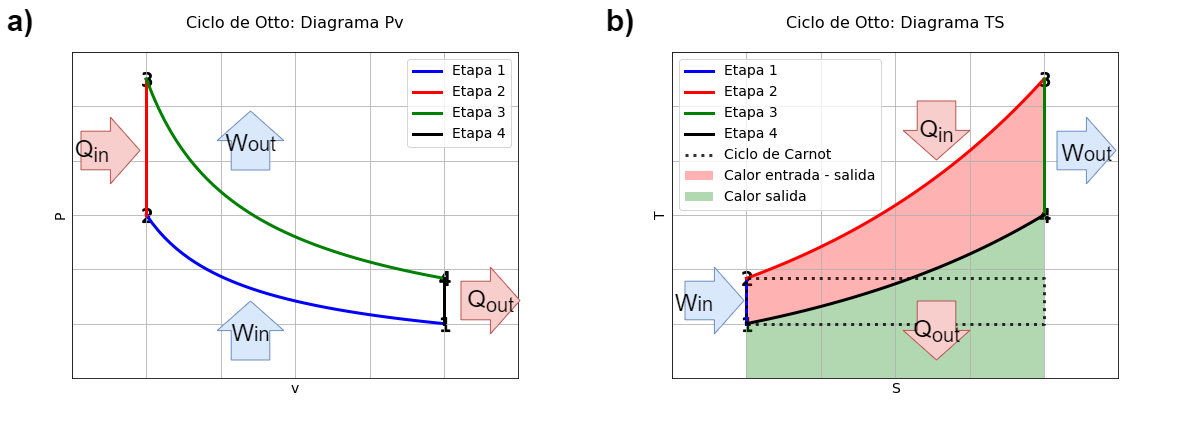
\includegraphics[width=.9\textwidth]{img/ciclos/ciclo_otto.png}
                \caption[Diagramas Ciclos de Otto]{\textbf{a)} Diagrama Pv y \textbf{b)} Diagrama TS del ciclo de Otto.}
                \label{fig:ciclo_otto}
            \end{figure}
            
            Etapas ciclo de Otto (\textbf{Figura \ref{fig:ciclo_otto}}):
            
            \begin{enumerate}
                \item \textbf{Etapa 1}: Compresión isoentrópica (Isoentrópico \(\Rightarrow\) Adiabático).
                \[\frac{T_{2}}{T_{1}}=\left ( \frac{v_{1}}{v_{2}} \right )^{\gamma - 1}\]
    
                \item \textbf{Etapa 2}: Admisión de calor a \(v=cte\):
                \[Q_{in}=Q_{23}=\int_{2}^{C}C_{v}dT=\bar{C_{v}}(T_{3}-T_{2})\]
                \[\wedge v_{2} = v_{3}\]
                
                \item \textbf{Etapa 3}: Expansión isoentrópica.
                \[\frac{T_{3}}{T_{4}}=\left ( \frac{v_{4}}{v_{3}} \right )^{\gamma - 1}\]
                
                \item \textbf{Etapa 4}: Eliminación de calor a \(v=cte\).
                \[Q_{out}=Q_{41}=\int_{4}^{A}C_{v}dT=-\bar{C_{v}}(T_{4}-T_{1})\]
                \[\wedge v_{4} = v_{1}\]
            \end{enumerate}
            \[\eta_{Otto}=\frac{Q_{in}-|Q_{out}|}{Q_{in}}=1-\frac{T_{4}-T_{1}}{T_{3}-T_{2}}=1-\frac{T_{1}\left ( \frac{T_{4}}{T_{1}} - 1\right )}{T_{2}\left ( \frac{T_{3}}{T_{2}} - 1\right )}\]
            
            Por las \(v=cte\) y los procesos adiabáticos:
            \[\frac{T_{2}}{T_{1}}=\frac{T_{3}}{T_{4}} \Leftrightarrow \frac{T_{4}}{T_{1}}=\frac{T_{3}}{T_{2}}\]
            \[\Rightarrow \eta_{Otto}=1-\frac{T_{1}}{T_{2}}\]
            
            Recordando \textbf{Etapa 1}:
            \[\frac{T_{1}}{T_{2}}=\left ( \frac{v_{2}}{v_{1}} \right)^{\gamma - 1}=\frac{1}{\left ( \frac{v_{1}}{v_{2}} \right)^{\gamma - 1}} \overset{\text{\textbf{Ecuación \ref{rel_comp}}}}{=} \frac{1}{r^{\gamma -1}}\]
            
            \begin{equation}
            \label{eficiencia_otto}
                \eta_{Otto}=1-\frac{1}{r^{\gamma -1}}
            \end{equation}
        
        \begin{figure}
            \centering
            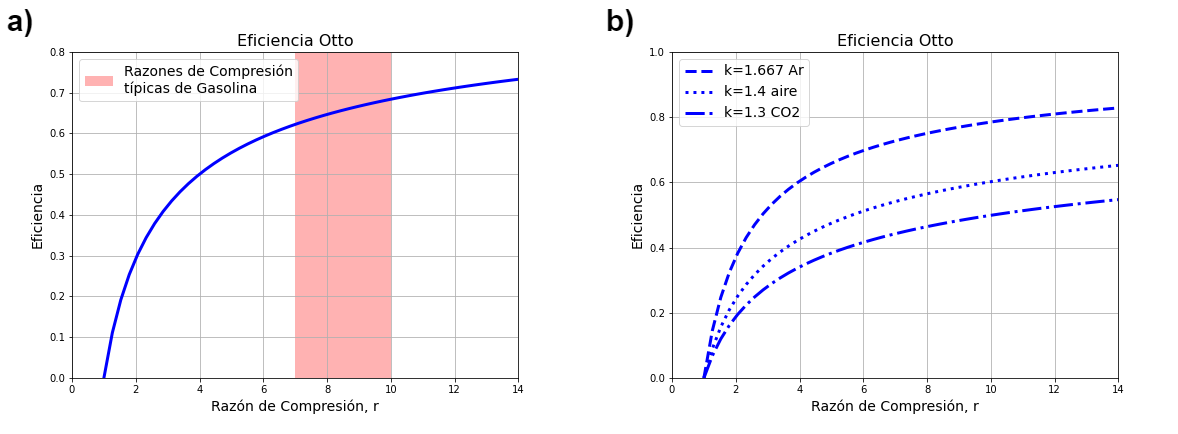
\includegraphics[width=\textwidth]{img/graficos/ef_otto.png}
            \caption[Eficiencia Otto]{Eficiencia Otto, con valores de \textbf{a)} Combustibles y \textbf{b)} diversos valores de \(\gamma\)}
            \label{fig:eff_otto}
        \end{figure}
            
        \subsubsection{Ciclo de Diesel}
        
            \subsubsubsection{Motor Diesel}
            
            \begin{multicols}{2}
                \begin{figure}[H]
                    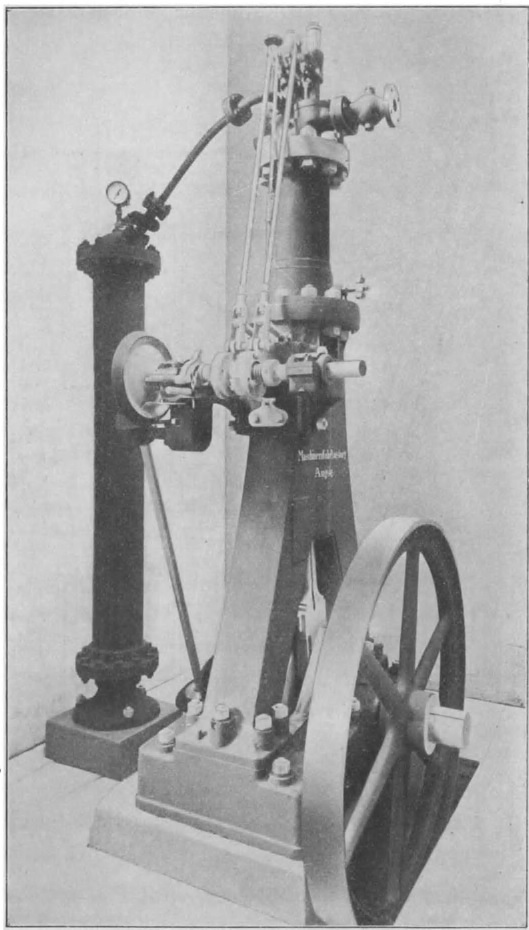
\includegraphics[width=.6\textwidth]{img/clases/motor_diesel.png}
                    \caption{Primer diseño experimental Diesel (Fuente: Clase 8)}
                    \label{fig:motor_diesel}
                \end{figure}
                
                El motor Diesel (\textbf{Figura \ref{fig:motor_diesel}}) (Rudolf Diesel, 1893):
                
                \begin{quote}
                    \textit{\say{Funciona mediante la \textbf{ignición (encendido) del combustible} al ser inyectado pulverizado y con alta presión en una cámara de combustión que contiene \textbf{aire a una temperatura superior} a la \textbf{temperatura de autocombustión}, sin necesidad de chispa como en los motores de gasolina. Este proceso es lo que se llama \textbf{autoinflamación}}}
                \end{quote}
            \end{multicols}
            
            \subsubsubsection{Ciclo Diesel Estándar}
            
            \begin{figure}
                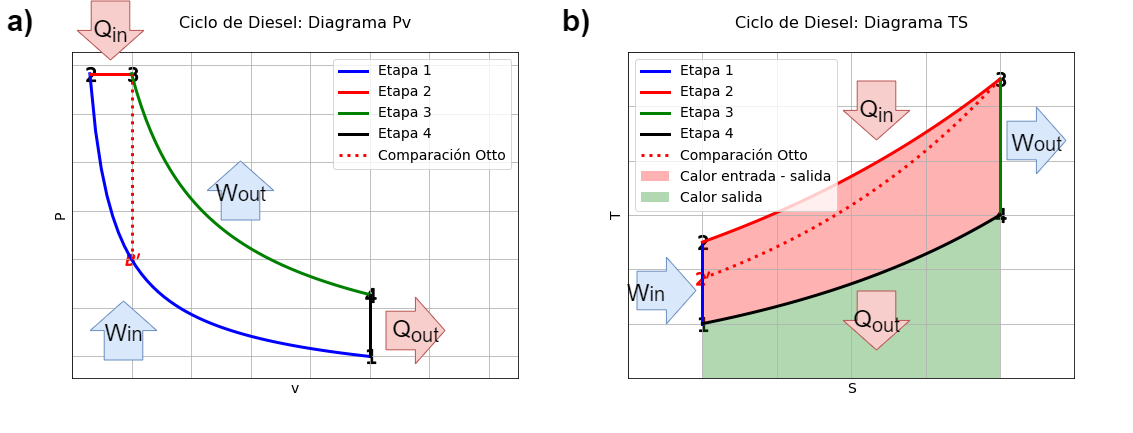
\includegraphics[width=\textwidth]{img/ciclos/ciclo_diesel.png}
                \caption[Diagramas Ciclos de Diesel]{\textbf{a)} Diagrama Pv y \textbf{b)} Diagrama TS del ciclo de Diesel}
                \label{fig:ciclo_diesel}
            \end{figure}
            
            Etapas ciclo de Diesel (\textbf{Figura \ref{fig:ciclo_diesel}}):
            
            \begin{enumerate}
                \item \textbf{Etapa 1}: Compresión isoentrópica.
                \item \textbf{Etapa 2}: Admisión de calor a \(P=cte\).
                \item \textbf{Etapa 3}: Expansión isoentrópica.
                \item \textbf{Etapa 4}: Eliminación de calor a \(v=cte\).
            \end{enumerate}
            
            Comparando la admisión de calor (Etapa 2) con el ciclo de Otto, se tiene:
            \[\overset{\text{Para Otto}}{\Rightarrow} \left ( \frac{\partial T}{\partial S} \right )_{v} = \frac{T}{C_{v}} \overset{\text{Para Diesel}}{\Rightarrow} \left ( \frac{\partial T}{\partial S} \right )_{P} = \frac{T}{C_{P}}\]
            
            Como \(C_{P} > C_{v} \Rightarrow \frac{1}{C_{P}} < \frac{1}{C_{v}}\), tenemos:
            \[\left ( \frac{\partial T}{\partial S} \right )_{v} > \left ( \frac{\partial T}{\partial S} \right )_{P}\]
            
            \[\eta_{Diesel} = \frac{Q_{in}-|Q_{out}|}{Q_{in}} = \frac{\bar{C_{P}}(T_{3}-T_{2})-\bar{C_{v}}(T_{4}-T_{1})}{\bar{C_{P}}(T_{3}-T_{2})}\]
            \[\eta_{Diesel} = 1-\frac{\bar{C_{v}}(T_{4}-T_{1})}{\bar{C_{P}}(T_{3}-T_{2})}=1-\frac{T_{4}-T_{1}}{\gamma (T_{3}-T_{2})}\]
            \[\overset{\frac{1}{T_{1}}}{\Rightarrow} \eta_{Diesel} = 1 - \frac{\frac{T_{4}}{T_{1}} - 1}{\gamma \left ( \frac{T_{3}}{T_{1}} - \frac{T_{2}}{T_{1}} \right )} = 1 - \frac{\frac{T_{4}}{T_{1}} - 1}{\gamma \frac{T_{2}}{T_{1}} \left ( \frac{T_{3}}{T_{2}} - 1 \right )}\]
            
            Como Etapas 1 son idénticas, recordando ciclo de Otto:
            \[\frac{T_{2}}{T_{1}}=r^{\gamma - 1}\]
            
            Considerando etapa 1 adiabática:
            \[\frac{P_{2}}{P_{1}}=\left ( \frac{v_{1}}{v_{2}} \right )^{\gamma} \wedge \frac{P_{3}}{P_{4}}=\left ( \frac{v_{4}}{v_{3}} \right )^{\gamma}\]
            
            Como \(v_{1}=v_{4}\) y \(P_{2}=P_{3}\)
            \[\frac{P_{2}}{P_{1}}=\left ( \frac{v_{1}}{v_{2}} \right )^{\gamma} \wedge \frac{P_{2}}{P_{4}}=\left ( \frac{v_{1}}{v_{3}} \right )^{\gamma}\]
            \[\Rightarrow \frac{P_{1}}{{v_{2}}^{\gamma}}=\frac{P_{4}}{{v_{3}}^{\gamma}} \Leftrightarrow \frac{P_{1}}{P_{4}}=\left ( \frac{v_{2}}{v_{3}} \right )^{\gamma}\]
            
            Como:
            \[\frac{P_{1}}{P_{4}} \overset{\text{\textbf{Ecuación \ref{gay_lussac}}}}{=} \frac{T_{1}}{T_{4}}=\left ( \frac{v_{2}}{v_{3}} \right )^{\gamma}\]
            \[\frac{T_{3}}{T_{2}} \overset{\text{\textbf{Ecuación \ref{charles}}}}{=} {\frac{v_{3}}{v_{2}}}\]
            
            \begin{multicols}{2}
                \begin{figure}
                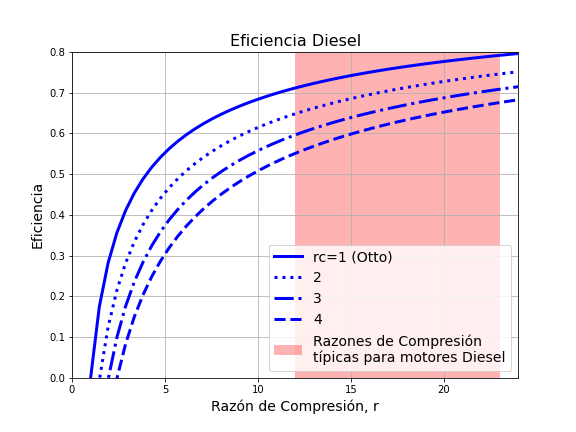
\includegraphics[width=\textwidth]{img/graficos/ef_diesel.png}
                    \caption{Eficiencia de Diesel}
                    \label{fig:ef_diesel}
                \end{figure}
                    
                Definiendo \textbf{Factor de admisión}:
                \begin{equation}
                \label{factor_adm}
                    r_{3} = \frac{v_{3}}{v_{2}}
                \end{equation}
                
                \begin{equation}
                \label{eficiencia_diesel}
                    \eta_{Diesel}=1-\frac{1}{r^{\gamma - 1}}\left ( \frac{{r_{3}}^{\gamma}-1}{\gamma (r_{3}-1)} \right )
                \end{equation}
            
                Como \(v_{3} > v_{2}\):
                \[r_{3} > 1 \overset{\gamma > 1}{\Rightarrow} {r_{3}}^{\gamma} > 1\]
                \[\overset{\text{Y}\cdots}{\Rightarrow} {r_{3}}^{\gamma} - 1 > \gamma (r_{3} - 1) \Rightarrow \frac{{r_{3}}^{\gamma} - 1}{\gamma (r_{3} - 1)} > 1 \Rightarrow \]
                \[\eta_{Diesel} < \eta_{Otto} \overset{r_{3} = 1}{\Rightarrow} \eta_{Diesel} = \eta_{Otto}\]
            \end{multicols}
    
    \subsection{Máquinas de Combustión Interna/Externa}
    
        \subsubsection{Motor Reciprocante de 2 tiempos}
        
        \begin{quote}
            \textit{\say{Menor eficiencia que los motores a 4 tiempos, principalmente debido a una expulsión incompleta de gases de combustión y una pérdida parcial de la mezcla aire- combustible. Más sencillos, económicos y livianos}}
        \end{quote}
        
            \subsubsubsection{Caballos de Vapor (CV)}
        
            \[1 [CV] = \frac{75 [kg] \cdot g \cdot 1 [m]}{1 [s]} = 714.75 [W] = 0.71475 [kW]\]
        
         \subsubsection{Ciclo Stirling}
         
            \subsubsubsection{Motor Stirling}
            
            \begin{figure}
                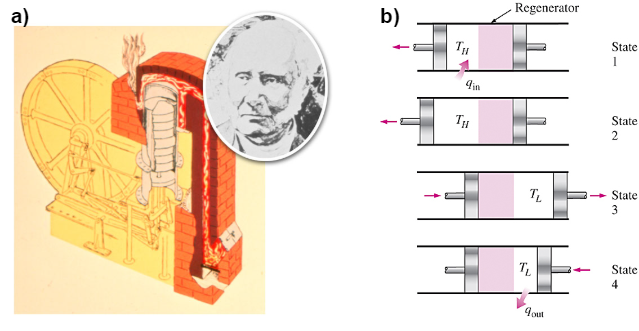
\includegraphics[width=\textwidth]{img/clases/stirling.png}
                \caption[Motor de Stirling]{\textbf{a)} Esquema del Motor de Stirling junto con una fotografía de Sir Robert Stirling. \textbf{b)} Esquema de los cuatro estados del ciclo. (Fuente: Clase 9)}
                \label{fig:stirling}
            \end{figure}
            
            El motor Stirling (\textbf{Figura \ref{fig:stirling}}) funciona mediante una \textbf{Fuente de Calor Externa} y un \textbf{Ciclo Cerrado} (Sir Robert Stirling, 1816).
            \newline
            
            \textbf{Fuente de Calor Externa}
                
            \begin{quote}
                \textit{\say{Motor intercambia el calor con el exterior. Adaptable a una gran gama de fuentes de calor. Proceso de combustión se puede controlar muy bien. Reducen las emisiones.}}
            \end{quote}
                
            \textbf{Ciclo Cerrado}
            
            \begin{quote}
                \textit{\say{Fluido de trabajo opera en un ciclo cerrado y la fuente de calor es externa. Potencialmente, de muy bajo nivel de emisiones}}
            \end{quote}
            
            \subsubsubsection{Ciclo Stirling Teórico}
            
            \begin{figure}
             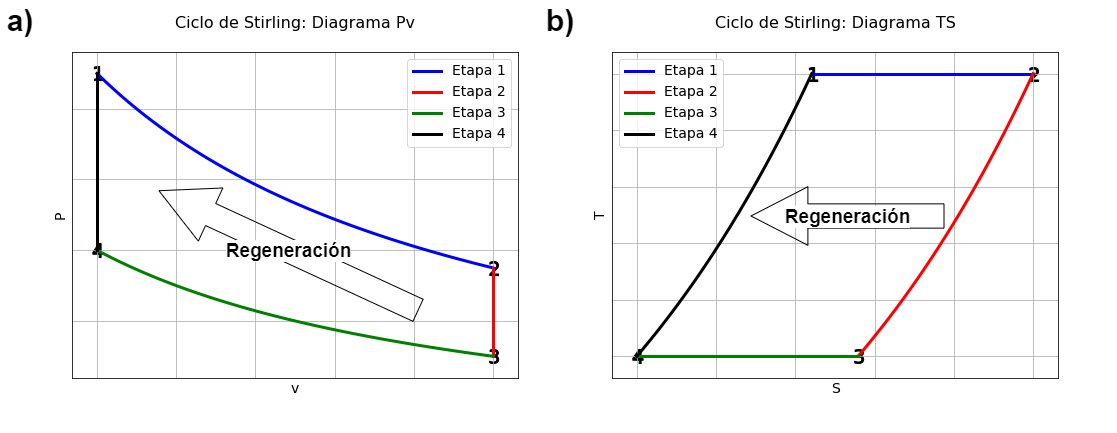
\includegraphics[width=\textwidth]{img/ciclos/ciclo_stirling.png}
                \caption[Ciclo de Stirling]{\textbf{a)} Diagrama Pv y \textbf{b)} Diagrama TS del ciclo de Stirling.}
                \label{fig:ciclo_stirling}
            \end{figure}
            
            Etapas del Ciclos de Stirling (\textbf{Figura \ref{fig:ciclo_stirling}}):
            
            \begin{enumerate}
                \item \textbf{Etapa 1}: Expansión isotérmica:
                \[Q_{in}=\int_{1}^{B}TdS = T_{H}(S_{2}-S_{1})=T_{H}R\ln(\frac{v_{2}}{v_{1}})\]
                \item \textbf{Etapa 2}: Compresión isocórica:
                \[v_{2}=v_{3}\]
                \item \textbf{Etapa 3}: Compresión isotérmica:
                \[Q_{out}=\int_{3}^{D}TdS = -T_{L}(S_{4}-S_{3})=-T_{L}R\ln(\frac{v_{3}}{v_{4}})\]
                \item \textbf{Etapa 4}: Expansión isocórica:
                \[v_{4}=v_{1}\]
            \end{enumerate}
            
            Calor transmitido através del regenerador (\(v=cte\)):
            \[|Q_{23}|=Q_{41}\]
            \[\eta_{Stirling}=\frac{Q_{in}-|Q_{out}|}{Q_{in}}=1-\frac{T_{L}R\ln(\frac{v_{3}}{v_{4}})}{T_{H}R\ln(\frac{v_{2}}{v_{1}})}\overset{v_{4}=v_{1}}{\Rightarrow}\;\overset{v_{2}=v_{3}}{\Rightarrow}\]
            \begin{equation}
            \label{eficiencia_stirling}
                \eta_{Stirling}=1-\frac{T_{L}}{T_{H}}
            \end{equation}
        
        \subsubsection{Turbinas y Ciclo Brayton}
        
            \subsubsubsection{Ciclo Ideal Brayton}
            
            \begin{figure}[H]
              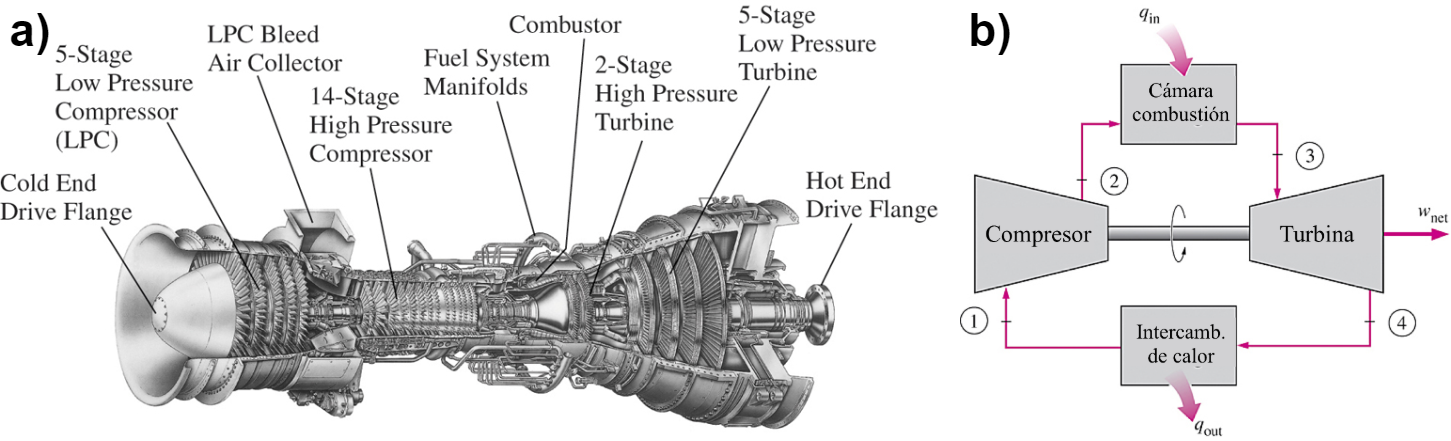
\includegraphics[width=\textwidth]{img/clases/turbinas.png}
                \caption[Esquema de Turbinas]{\textbf{a)} Esquema del funcionamiento de una Turbina. \textbf{b)} Esquema de las partes de una Turbina y su relación con el ciclo Ideal de Brayton (Fuente: Clase 9).}
                \label{fig:turbinas}
            \end{figure}
            
            \begin{figure}
                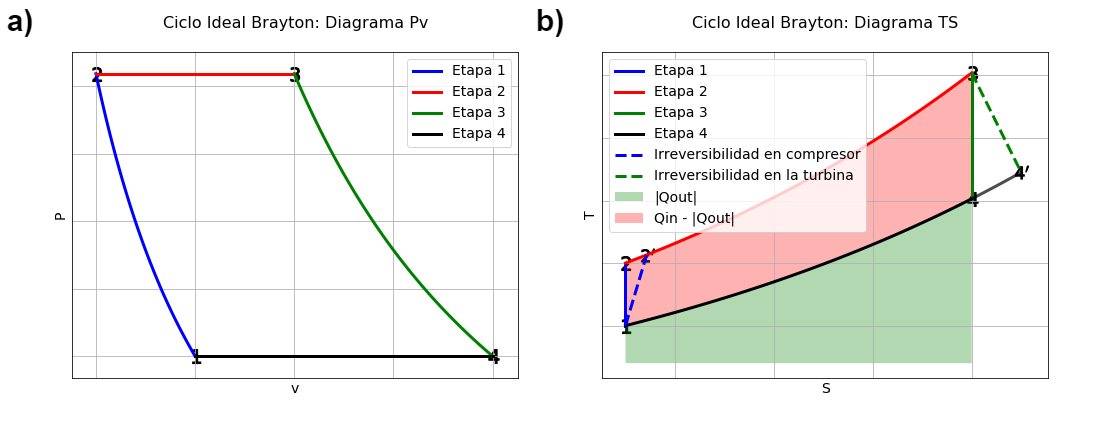
\includegraphics[width=\textwidth]{img/ciclos/ciclo_brayton.png}
                \caption[Ciclo Ideal de Brayton]{\textbf{a)} Diagrama Pv y \textbf{b)} Diagrama TS del ciclo Ideal de Brayton.}
                \label{fig:ciclo_brayton}
            \end{figure}
            
            Etapas del Ciclos de Brayton (\textbf{Figura \ref{fig:ciclo_brayton}}):
            
            \begin{enumerate}
                \item \textbf{Etapa 1}: Compresión isoentrópica:
                \[P_{1}{v_{1}}^{\gamma}=P_{2}{v_{2}}^{\gamma}\]
                \[T_{1}{v_{1}}^{\gamma - 1}=T_{2}{v_{2}}^{\gamma - 1} \Rightarrow \frac{T_{2}}{T_{1}}=\left ( \frac{v_{1}}{v_{2}} \right )^{\gamma - 1}\]
                \[\frac{T_{2}}{T_{1}}=\left ( \frac{P_{2}}{P_{1}} \right )^{\frac{\gamma - 1}{\gamma}}\]
                
                \item \textbf{Etapa 2}: Adición de calor en proceso isobárico:
                \[Q_{in}=C_{P}(T_{3}-T_{2})\]
                
                \item \textbf{Etapa 3}: Expansión isoentrópica:
                \[\frac{T_{3}}{T_{4}}=\left ( \frac{P_{3}}{P_{4}} \right )^{\frac{\gamma - 1}{\gamma}}=\left ( \frac{P_{2}}{P_{1}} \right )^{\frac{\gamma-1}{\gamma}}\]
                
                \item \textbf{Etapa 4}: Rechazo de calor en proceso isobárico:
                \[Q_{out}=-C_{P}(T_{1} -T_{4})\]
            \end{enumerate}
            
            \begin{multicols}{2}
            Eficiencia del ciclo ideal de Brayton:
            \[\eta_{Brayton}=1-\frac{|Q_{out}|}{Q_{in}}=1-\frac{T_{4}-T_{1}}{T_{3}-T_{2}}\]
            \[\eta_{Brayton}=1-\frac{T_{1}\left ( \frac{T_{4}}{T_{1}} - 1 \right )}{T_{2}\left ( \frac{T_{3}}{T_{2}} - 1 \right )}\]
            
            Igualando las etapas 1 y 3:
            \[\frac{T_{2}}{T_{1}}=\frac{T_{3}}{T_{4}} \Rightarrow \frac{T_{4}}{T_{1}}=\frac{T_{3}}{T_{2}} \Rightarrow \frac{T_{4}}{T_{1}} - 1=\frac{T_{3}}{T_{2}} - 1\]
            
            Definiendo \textbf{Relación de presiones}:
            \begin{equation}
            \label{def_rel_pres}
                r_{P} = \frac{P_{2}}{P_{1}}    
            \end{equation}
            
            \begin{figure}
                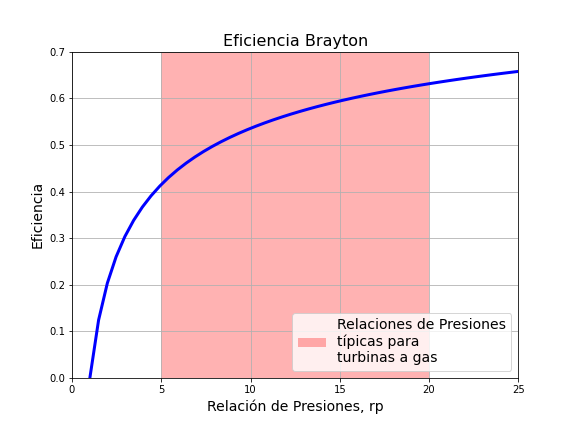
\includegraphics[width=\textwidth]{img/graficos/ef_brayton_turbinas.png}
                \caption[Eficiencia ciclo Ideal de Brayton]{Eficiencia del ciclo Ideal de Brayton a diferentes \(r_{P}\) típicas de turbinas.}
                \label{fig:ef_brayton}
            \end{figure}
            \end{multicols}
            
            Finalmente:
            \begin{equation}
            \label{ef_brayton}
                \eta_{Brayton}=1-\frac{1}{{r_{P}}^{\frac{\gamma - 1}{\gamma}}}
            \end{equation}
            
            En la \textbf{Figura \ref{fig:ciclo_brayton}.b} se ve que en la realidad hay irreversibilidades que disminuyen la eficiencia:
            \begin{multicols}{2}
            \begin{equation}
            \label{irr_compr}
                \eta_{compresor}=\frac{w_{ideal}}{w_{real}}=\frac{h_{2}-h_{1}}{h_{B'}-h_{1}}
            \end{equation}
            
            \begin{equation}
            \label{irr_turb}
                \eta_{turbina}=\frac{w_{real}}{w_{ideal}}=\frac{h_{3}-h_{D'}}{h_{3}-h_{4}}
            \end{equation}
            \end{multicols}
            
            \subsubsubsection{Ciclo Brayton con Regeneración}
            
            \begin{figure}
                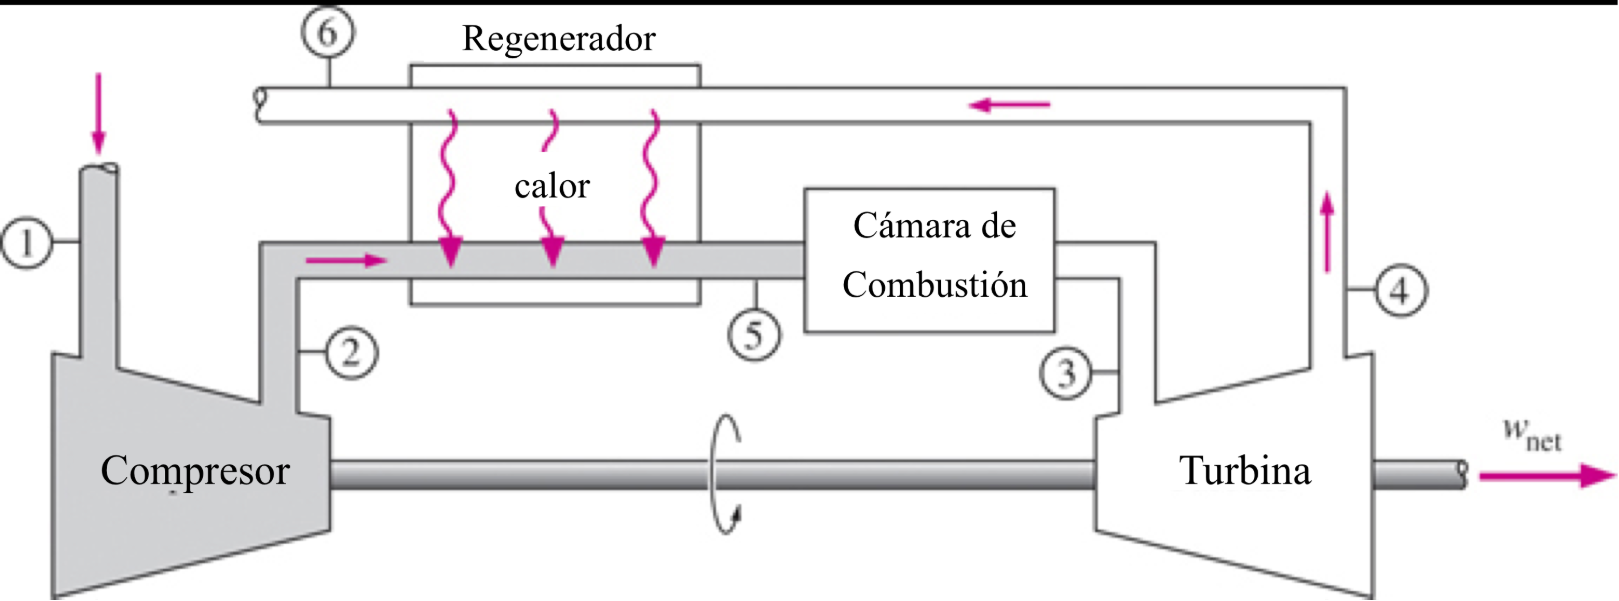
\includegraphics[width=\textwidth]{img/clases/turbina_reg.png}
                \caption{Esquema de una Turbina con regeneración. (Fuente: Clase 9).}
                \label{fig:turbina_reg}
            \end{figure}
            
            \begin{multicols}{2}
                \begin{figure}
                    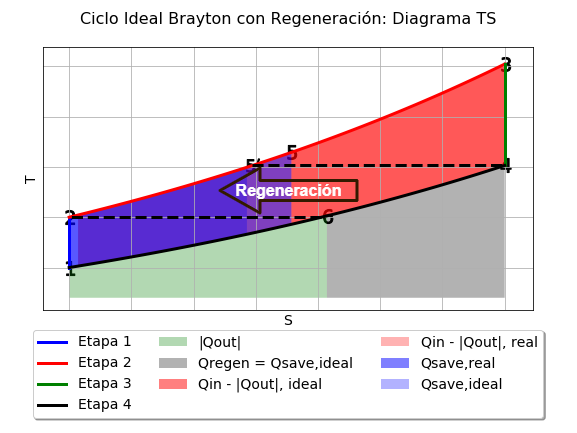
\includegraphics[width=\textwidth]{img/ciclos/ciclo_brayton_reg.png}
                    \caption{Ciclo de Brayton con Regeneración}
                    \label{fig:ciclo_brayton_reg}
                \end{figure}
                
                \begin{figure}
                    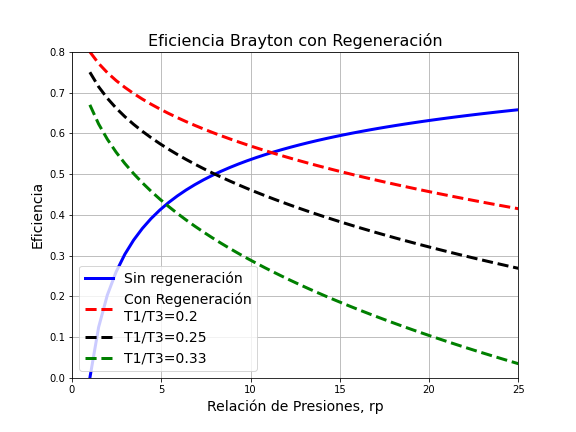
\includegraphics[width=\textwidth]{img/graficos/ef_brayton_reg.png}
                    \caption{Eficiencia Ciclo de Brayton con Regeneración}
                    \label{fig:ef_brayton_reg}
                \end{figure}
                
            \end{multicols}
                
            Eficiencia de regeneración \(\epsilon\):
            \begin{equation}
            \label{ef_reg}
                \epsilon = \frac{q_{(regen, real)}}{q_{(regen, ideal)}} = \frac{h_{5}-h_{2}}{h_{5'}-h_{2}} \approx \frac{T_{5}-T_{2}}{T_{4}-T_{2}}
            \end{equation}
            
            \begin{equation}
            \label{ef_brayton_reg}
                \eta_{(Brayton, regen)} = 1 - \frac{T_{1}}{T_{3}}{r_{P}}^{\frac{1-\gamma}{\gamma}}
            \end{equation}
            
            \subsubsubsection{Ciclo Brayton con Regeneración, \textit{inter}enfriamiento y \textit{re}calentamiento}
            
            \begin{figure}
                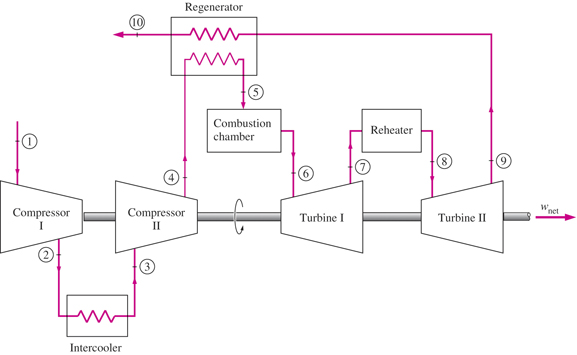
\includegraphics[width=\textwidth]{img/clases/turbina_inter_recal.png}
                \caption{Esquema de una turbina con regeneración, inter-enfriamiento y re-calentamiento}
                \label{fig:turbina_inter_recal}
            \end{figure}
            
            \begin{figure}
                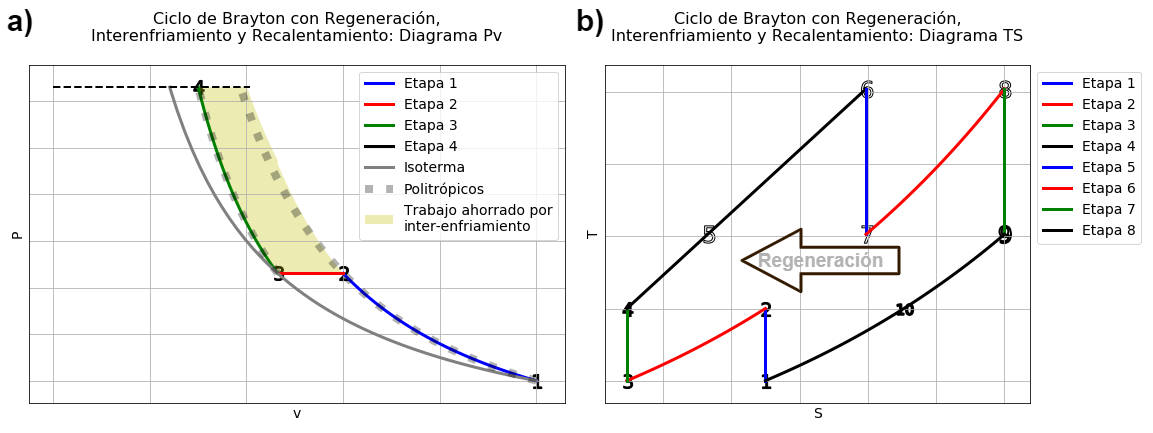
\includegraphics[width=\textwidth]{img/ciclos/ciclo_brayton_reg_enfr.png}
                \caption[Ciclo de Brayton con Regeneración, inter-enfriamiento y re-calentamiento]{Ciclo de Brayton con Regeneración, inter-enfriamiento y re-calentamiento. \textbf{a)} Diagrama Pv. \textbf{b)} Diagrama TS.}
                \label{fig:ciclo_brayton_inter_rec}
            \end{figure}
            \newpage
            
        \subsubsection{Celdas de Combustible}
        
        \begin{multicols}{2}
        
        \begin{quote}
            \textit{\say{En reacciones químicas, la irreversibilidad se debe al intercambio incontrolado de electrones entre los componentes reactivos. El intercambio de electrones puede controlarse al sustituir la cámara de combustión por celdas electrolíticas, como las baterías de automóvil. (Esto es análogo a reemplazar la expansión libre de un gas en sistemas mecánicos por expansión controlada.) En las celdas electrolíticas, los electrones se intercambian mediante alambres conductores conectados a una carga, y la energía química se convierte directamente en energía eléctrica. Los dispositivos de conversión de energía que trabajan con base en este principio se llaman celdas de combustible.}} \cite{cengel_termodinamica_2012}.
        \end{quote}
        
        \begin{figure}
            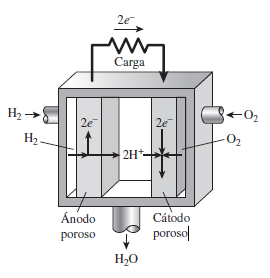
\includegraphics{img/clases/celdas_combustible.png}
            \caption{Esquema de una Celda de Combustible de Hidrógeno y Oxígeno (Fuente: Termodinámica Séptima Edición)}
            \label{fig:celdas_conbustibles}
        \end{figure}
        
        \end{multicols}
    
    \subsection{Ciclos de Vapor}
        
        \subsubsection{Centrales Termoeléctricas}
        
            \subsubsubsection{Centrales termoeléctricas convencionales}
            
            \begin{quote}
                \textit{\say{Utilizan combustibles fósiles para obtener elevadas temperaturas necesarias para producir vapor de agua.}}
            \end{quote}
            
            \begin{table}[H]
            \caption{Tabla de emisiones de \(CO_{2}\) para diferentes combustibles}
            \label{tabla_emision_co2}
                \begin{tabular}{|l|c|}
                    \hline
                    \rowcolor[HTML]{FE0000} {\color[HTML]{FFFFFF} \textbf{Combustible}} & {\color[HTML]{FFFFFF} \textbf{Emisión de \(CO_{2}\) \(\left [ \frac{kg}{kWh} \right ]\)}} \\ \hline
                    Gas Natural                                 & \(0.44\)                                                                                                          \\ \hline
                    Combustibles fósiles                        & \(0.71\)                                                                                                          \\ \hline
                    Biomasa                                     & \(0.82\)                                                                                                          \\ \hline
                    Carbón                                      & \(1.45\)                                                                                                          \\ \hline
                \end{tabular}
            \end{table}
            
            \begin{figure}[H]
                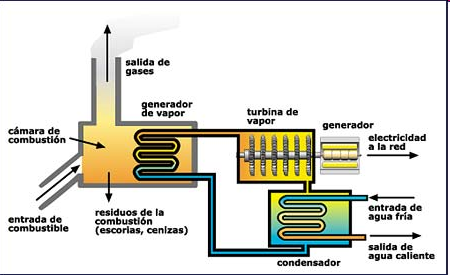
\includegraphics[width=\textwidth]{img/clases/centrales_termoelectricas_convencionales.png}
                \caption{Esquema de una central termoeléctrica convencional (Fuente: Clase 10).}
                \label{fig:central_convencional}
            \end{figure}
            
            \begin{figure}[H]
                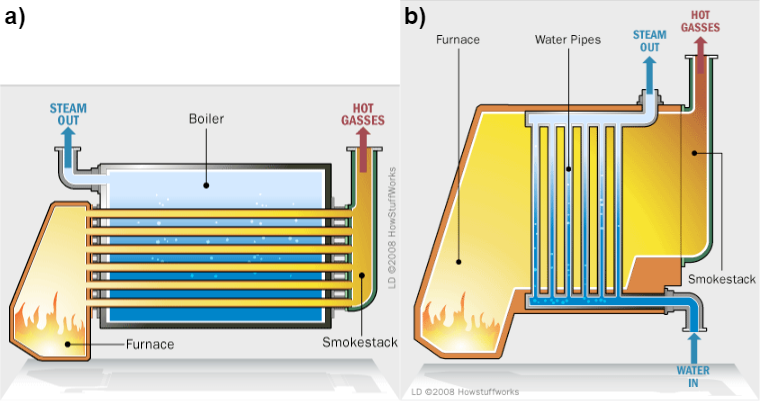
\includegraphics[width=\textwidth]{img/clases/caldera.png}
                \caption[Esquema de calderas (Fuente: Clase 10)]{\textbf{a)} Esquema de una caldera {\color[HTML]{FE0000}Piro}tubular. \textbf{b)} Esquema de una caldera {\color[HTML]{0000FE}Acuo}tubular. (Fuente: Clase 10).}
                \label{fig:central_convencional_2}
            \end{figure}
        
        \subsubsection{Ciclo de Carnot}
        
        Usando vapor en el ciclo de Carnot dentro de la campana de saturación (\textbf{Figura \ref{fig:ciclo_carnot_ts}.a}) se tiene:
        
        \begin{multicols}{2}
            \begin{enumerate}
                \item \textbf{Etapa 1}: Absorción de calor en proceso isotérmico. Estando dentro de la campana de saturación también es isobárico.
                \item \textbf{Etapa 2}: Expansión adiabática y reversible (isoentrópica) en la turbina.
                \item \textbf{Etapa 3}: Condensación parcial en proceso isotérmico (isobárico al estar dentro de la campana).
                \item \textbf{Etapa 4}: Compresión isoentrópica de vapor húmedo.
            \end{enumerate}
        \end{multicols}
        
        Problemas:
        
        \begin{multicols}{2}
            \begin{enumerate}
                \item Erosión de los álabes de la turbina (\textbf{Etapa 2}).
                \item Dificultad de comprimir vapor húmedo (\textbf{Etapa 4}).
                \item Para evitarlo podemos usar mayores temperaturas (\textbf{Figura \ref{fig:ciclo_carnot_ts}.b}), pero estariamos en la zona supercrítica.
            \end{enumerate}
        \end{multicols}
        
        \begin{figure}
            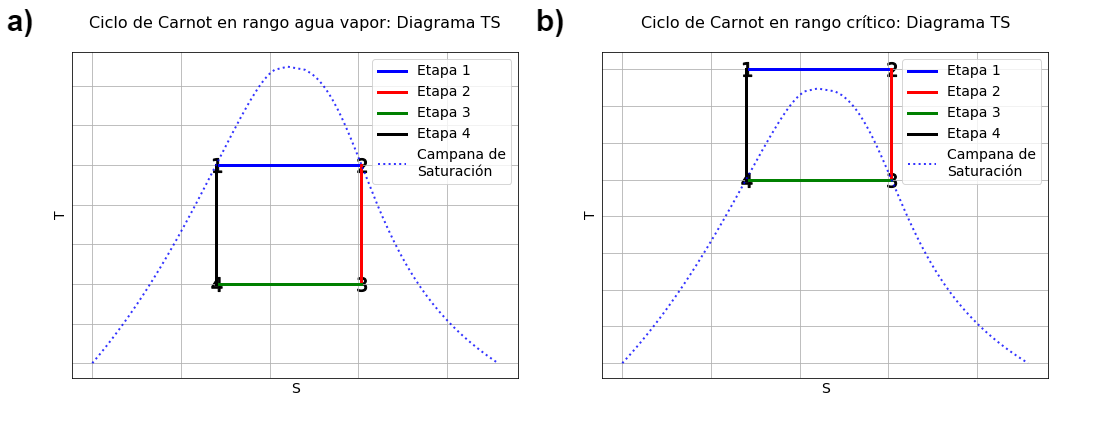
\includegraphics[width=\textwidth]{img/ciclos/ciclo_carnot_ts.png}
            \caption[Diagramas TS del ciclo de Carnot]{Diagramas TS del ciclo de Carnot. \textbf{a)} Ciclo dentro de la campana de saturación. \textbf{b)} Ciclo cercano al punto crítico.}
            \label{fig:ciclo_carnot_ts}
        \end{figure}
        
        \subsubsection{Ciclo de Rankine}
        
        Publicado en \textit{Manual of Steam Engine} (William J.M. Rankine, 1859). Modificación del ciclo de Carnot (\textbf{Figura \ref{fig:ciclo_carnot_ts}.a}), considera (\textbf{Figura \ref{fig:ciclo_rankine_esquema}} y \textbf{Figura \ref{fig:ciclo_rankine}.a}):
        \newpage
        
        \begin{multicols}{2}
            \begin{enumerate}
                \item \textbf{Etapa 1}: Compresión isoentrópica en la bomba.
                \[q = 0 \wedge w_{in \text{ (bomba)}} = h_{2} - h_{1} = v(P_{2} - P_{1})\]
                
                Con \(h_{1}=h_{f}(P_{1})\), \(v \approx v_{1} = v_{f}(P_{1})\).
                
                \item \textbf{Etapa 2}: Adición de calor isobárica en caldera.
                \[w = 0 \wedge q_{in} = h_{3} - h_{2}\]
                
                \item \textbf{Etapa 3}: Expansión isoentrópica en turbina.
                \[q = 0 \wedge w_{out \text{ (turbina)}} = h_{3} - h_{4}\]
                
                \item \textbf{Etapa 4}: Rechazo de calor isobático en un condensador.
                \[w = 0 \wedge q_{out} = h_{4} - h_{1}\]
            \end{enumerate}
            
            \begin{figure}
                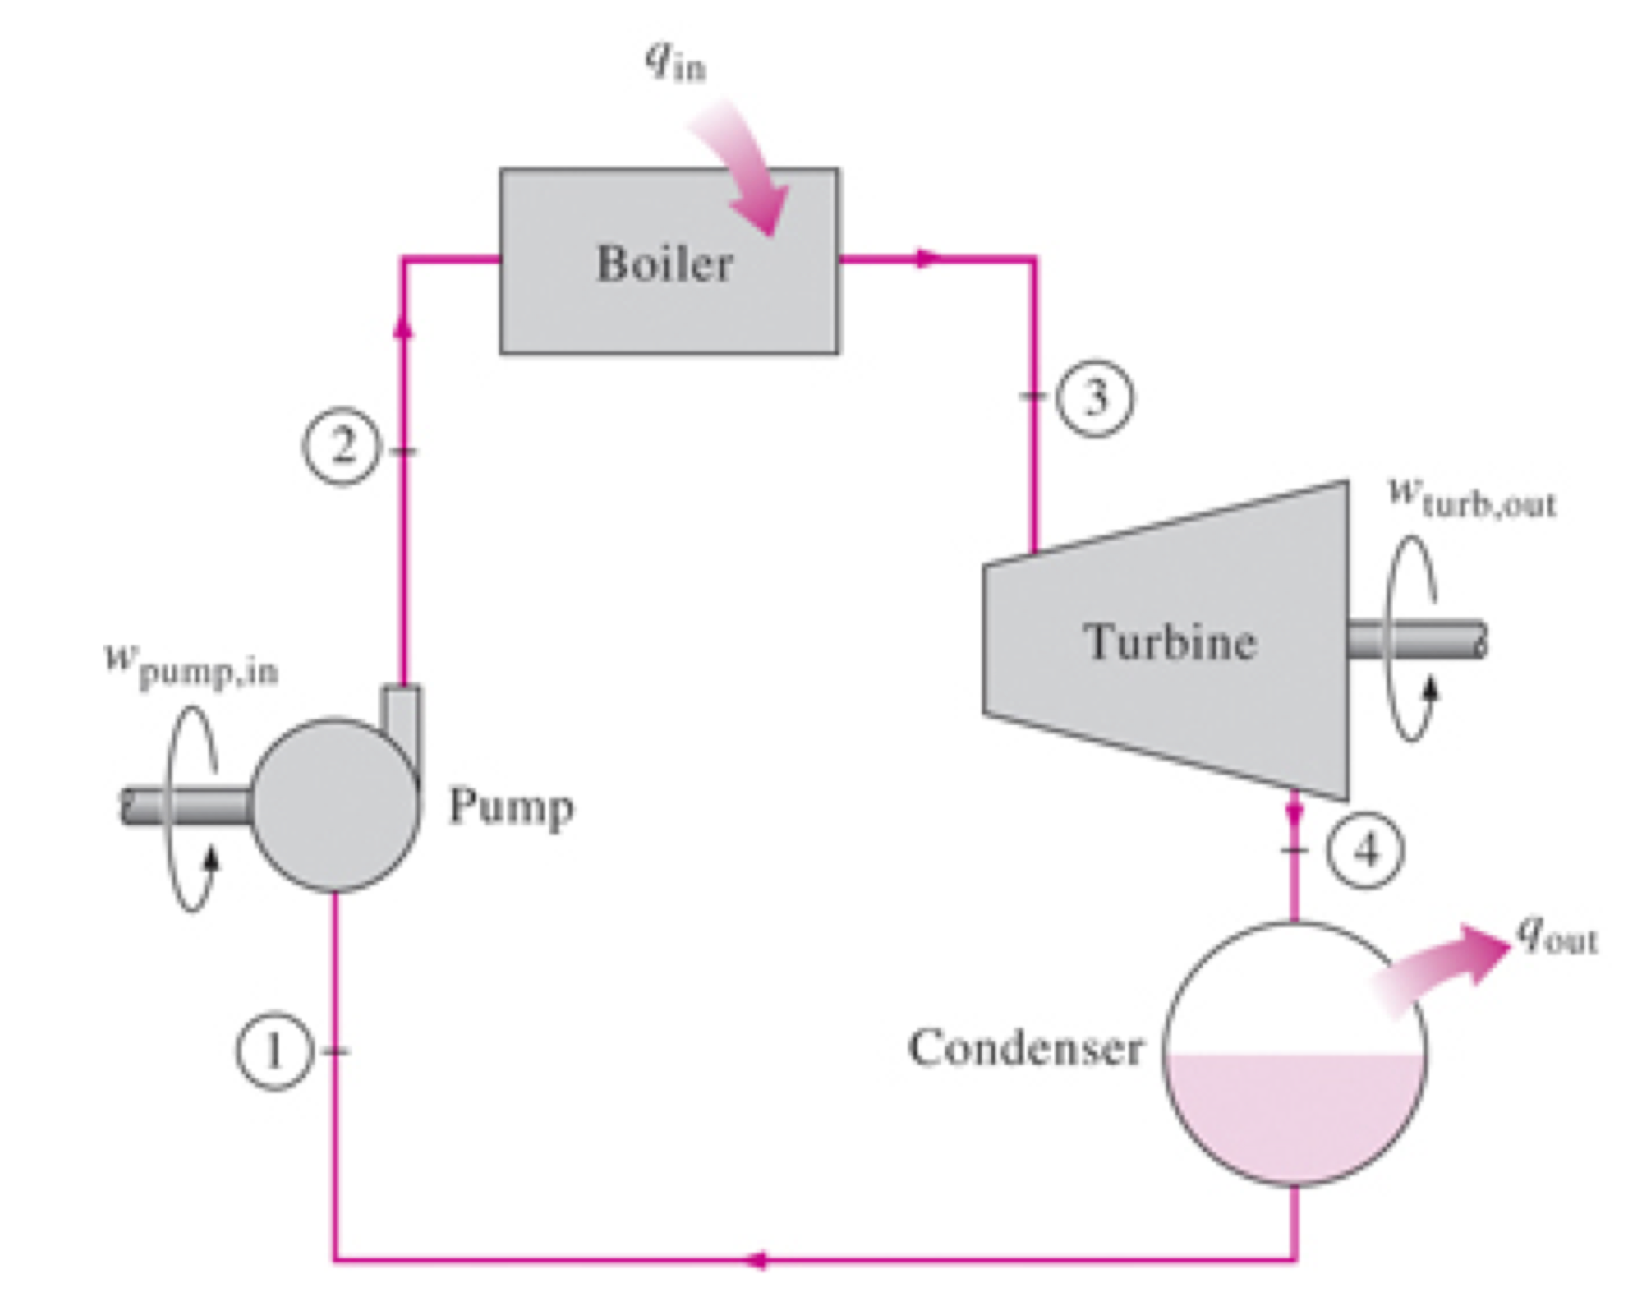
\includegraphics[width=\textwidth]{img/clases/ciclo_rankine_esquema.png}
                \caption{Esquema de una máquina de vapor que usa el ciclo de Rankine (Fuente: Clase 10).}
                \label{fig:ciclo_rankine_esquema}
            \end{figure}
        \end{multicols}
        
        \begin{figure}
            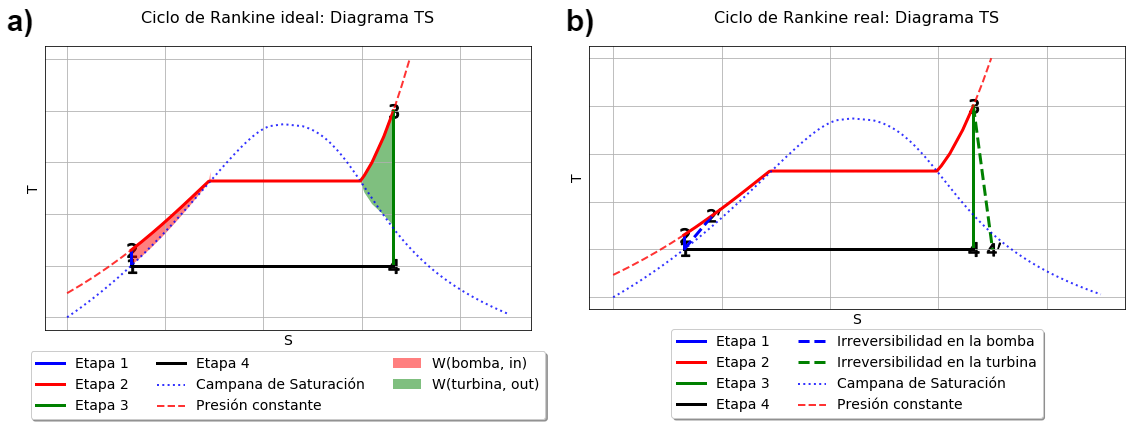
\includegraphics[width=\textwidth]{img/ciclos/ciclo_rankine.png}
            \caption[Diagrama TS del Ciclo de Rankine]{\textbf{a)} Diagrama TS del ciclo ideal de Rankine. \textbf{b)} Diagrama TS que muestra irreversibilidades en el Ciclo}
            \label{fig:ciclo_rankine}
        \end{figure}
        
        \[n_{Rankine, Ideal}=\frac{w_{neto}}{q_{in}}=\frac{w_{\text{turbina}}-|w_{\text{bomba}}|}{q_{in}}=\frac{q_{\text{caldera}}-|q_{\text{condensador}}|}{q_{\text{caldera}}}\]
        \begin{equation}
        \label{ef_rankine_ideal}
            \eta_{Rankine, ideal} = 1 - \frac{h_{4}-h_{1}}{h_{3}-h_{2}}
        \end{equation}
        
        Dado irreversibilidades en la bomba y turbina (\textbf{Figura \ref{fig:ciclo_rankine}.b}). Se tiene:
        \[\text{Bomba: }P_{(2, ideal)}=P_{(2, real)} \Rightarrow S_{(2, real)}>S_{(2, ideal)}\]
        \[\text{Turbina: }P_{(4, ideal)}=P_{(4, real)} \Rightarrow S_{(4, real)}>S_{(4, ideal)}\]
        \[\text{Eficiencia isoentrópica }\eta_{S}=\frac{W_{real}}{W_{S=cte}}\]
        \begin{equation}
        \label{ef_rankine_isoentropica}
            \eta_{S} = \frac{h_{3} - h_{4, real}}{h_{3} - h_{4, ideal}}
        \end{equation}
        
            \subsubsubsection{Aumento de la Eficiencia}
            
            \begin{figure}
                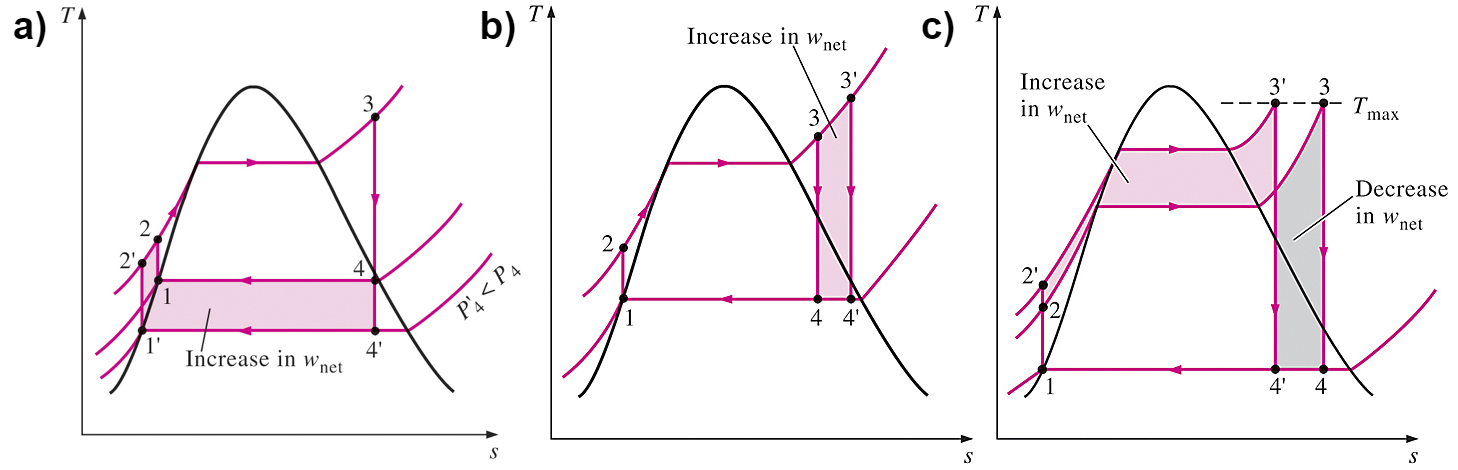
\includegraphics[width=\textwidth]{img/clases/aumento_eficiencia_rankine.png}
                \caption[Aumento de la eficiencia del ciclo de Rankine (Fuente: Clase 10)]{Aumento de la eficiencia del ciclo de Rankine. \textbf{a)} Reducción de la presión del condensador. \textbf{b)} Sobrecalentamiento del vapor a altas temperaturas. \textbf{c)} Incremento de la presión de la caldera (Fuente: Clase 10).}
                \label{fig:rankine_mas_ef}
            \end{figure}
            
            \textbf{Reducción de la presión del condensador (\textbf{Figura \ref{fig:rankine_mas_ef}.a}):}
            
            \begin{quote}
                \textit{\say{... se reduce automáticamente la temperatura del vapor, y por lo tanto la temperatura a la cual el calor es rechazado.}}
            \end{quote}
            
            \textbf{Sobrecalentamiento del vapor a altas temperaturas (\textbf{Figura \ref{fig:rankine_mas_ef}.b}):}
            
            \begin{quote}
                \textit{\say{...disminuye el contenido de humedad del vapor a la salida de la turbina.}}
            \end{quote}
            
            \begin{quote}
                \textit{\say{Sin embargo, la temperatura a la que el vapor se sobrecalienta está limitada debido a consideraciones metalúrgicas, aproximadamente \(620 [{}^{o}C]\) (\(1150 [{}^{o}F]\)).}}
            \end{quote}
            \newpage
            
            \textbf{Incremento de la presión en la Caldera (\textbf{Figura \ref{fig:rankine_mas_ef}.c}):}
            
            \begin{quote}
                \textit{\say{...se eleva la temperatura de ebullición, lo que a su vez eleva la temperatura promedio de transferencia de calor al vapor.}}
            \end{quote}
            
            \begin{quote}
                \textit{\say{Para una misma temperatura de entrada a la turbina, el ciclo se mueve a la izquierda, aumentando el contenido de humedad del vapor en la salida de la turbina. Esto se puede corregir con un proceso de \textbf{recalentamiento}.}}
            \end{quote}
    
        \subsubsection{Ciclo de Rankine con Recalentamiento}
        
        \begin{figure}
            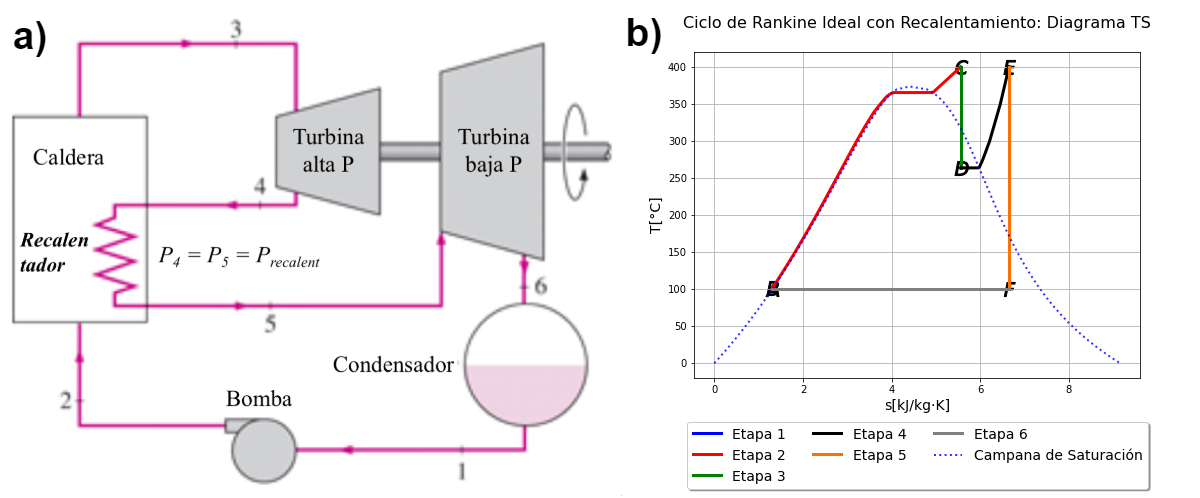
\includegraphics[width=\textwidth]{img/ciclos/ciclo_rankine_recal.png}
            \caption[Ciclo de Rankine con Recalentamiento]{\textbf{a)} Esquema del Recalentamiento en un Ciclo de Rankine (Fuente: Clase 10). \textbf{b)} Diagrama TS del Ciclo de Rankine (Ideal) con Recalentamiento.}
            \label{fig:ciclo_rankine_recal}
        \end{figure}
        
        \begin{equation}
        \label{ef_rankine_recal}
            \eta_{Rankine, Recal} = 1 - \frac{h_{6}-h_{1}}{(h_{3}-h_{2})-(h_{5}-h_{4})}
        \end{equation}
        
        \subsubsection{Ciclo Rankine Regenerativo}
        
        \begin{quote}
            \textit{\say{Un proceso de regeneración se logra con la extracción (\say{drenado} o \say{purga}) del vapor de la turbina en diversos puntos. Este vapor, que podría producir más trabajo, se utiliza en cambio para calentar el agua de alimentación.}}
        \end{quote}
        
        \begin{figure}
            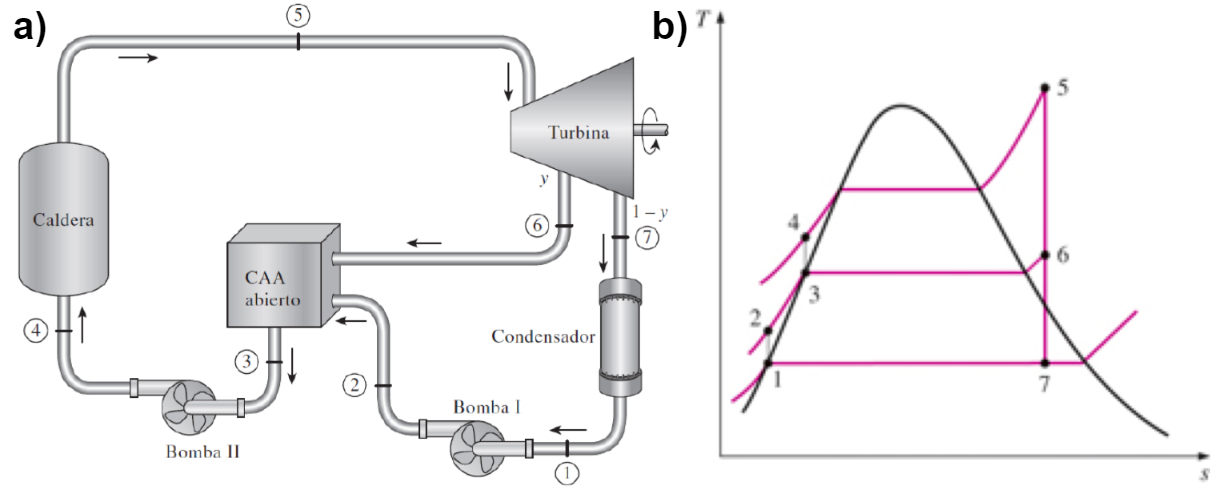
\includegraphics[width=.8\textwidth]{img/clases/ciclo_rankine_reg.png}
            \caption[Ciclo Rankine Regenerativo (Fuente: Clase 10)]{\textbf{a)} Esquema del Ciclo Rankine Regenerativo. \textbf{b)} Diagrama TS del Ciclo de Rankine Regenerativo. (Fuente: Clase 10).}
            \label{fig:ciclo_rankine_reg}
        \end{figure}
        
            \subsubsubsection{Calentador de Agua de Alimentación (CAA)}
            
            \begin{itemize}
                \item \textbf{CAA Abierto}:
                
                \begin{quote}
                    \textit{\say{...vapor extraído de la turbina se mezcla con el agua de alimentación que sale de la bomba. La mezcla sale del calentador como liquido saturado a la presión del calentador.}}
                \end{quote}
                
                \item \textbf{CAA Cerrado}:
                
                \begin{quote}
                    \textit{\say{El calor se transfiere del vapor extraído hacia el agua de alimentación sin que suceda ninguna mezcla. Los dos flujos pueden estar a presiones diferentes, puesto que no se mezclan}}
                \end{quote}
                
            \end{itemize}
            
            \subsubsubsection{Trabajo generado}
            
            Desde (\textbf{Figura \ref{fig:ciclo_rankine_reg}}):
            \[y = \frac{\dot{m_{6}}}{\dot{m_{5}}} \text{ fracción de vapor extraído} \Rightarrow q_{in} = h_{5} - h_{4} \wedge q_{out} = (1 - y)(h_{7} - h_{1})\]
            \[w_{out \text{ (turbina)}} = (h_{5} - h_{6}) + (1 - y)(h_{6} - h_{7)} \wedge w_{in \text{ (bombas)}} = (1 - y)w_{in \text{ (bomba 1)}} + w_{in \text{ (bomba 2)}}\]
            \[w_{in \text{ (bomba 1)}} = v_{1}(P_{2}-P_{1}) \wedge w_{in \text{ (bomba 2)}} = v_{3}(P_{4}-P_{3})\]
        
        \subsubsection{Ciclo Combinado}
        
            \subsubsubsection{Idea}
            
            \begin{quote}
                \textit{\say{Combinación de dos ciclos de Rankine: uno con fluido motor mercurio (alta temperatura) y otro con agua (baja temperatura).}}
            \end{quote}
            
            \begin{figure}
                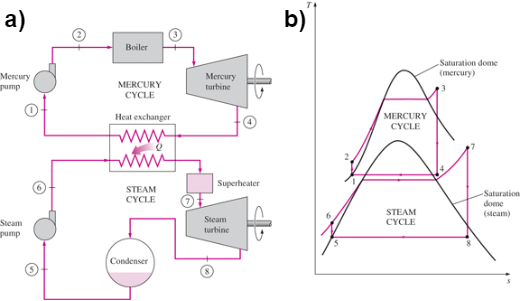
\includegraphics[width=.75\textwidth]{img/clases/ciclo_rankine_combinado.png}
                \caption[Ciclo Rankine Combinado]{\textbf{a)} Esquema de un Ciclo Rankine Combinado. \textbf{b)} Diagrama TS del ciclo. (Fuente: Clase 10).}
                \label{fig:ciclo_rankine_comb}
            \end{figure}
            
            \subsubsubsection{Actuales}
            
            \begin{figure}
                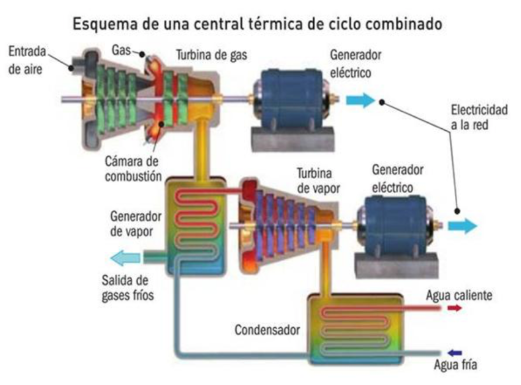
\includegraphics[width=.65\textwidth]{img/clases/central_termoelectrica_esquema.png}
                \caption{Esquema de una central térmica de ciclo combinado (Fuente: Clase 10).}
                \label{fig:esquema_ciclo_combinado}
            \end{figure}
            
            Dos ciclos:
            
            \begin{enumerate}
                \item \textbf{Brayton}: producción de trabajo con alta eficiencia en rangos altos de temperaturas de trabajo.
                \item \textbf{Rankine}: temperaturas medias-bajas.
            \end{enumerate}
            
            \begin{figure}
                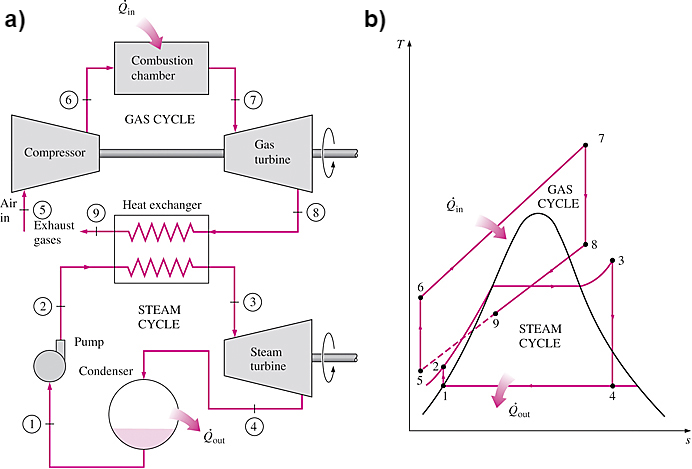
\includegraphics[width=.7\textwidth]{img/clases/ciclo_combinado.png}
                \caption[Ciclo Combinado]{\textbf{a)} Esquema de un Ciclo Combinado. \textbf{b)} Diagrama TS del ciclo. (Fuente: Clase 10).}
                \label{fig:ciclo_combinado}
            \end{figure}
        
        \subsubsection{Central Geotérmica}
        
        \begin{figure}
            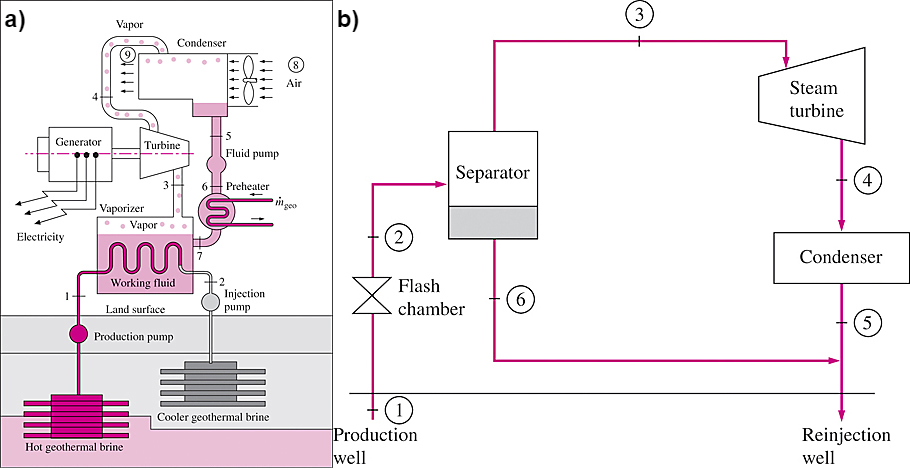
\includegraphics[width=\textwidth]{img/clases/esquema_central_geotermica.png}
            \caption[Central Geotérmica (Fuente: Clase 10)]{\textbf{a)} Esquema de una central geotérmica. \textbf{b)} Esquema de las etapas del vapor en una central geotérmica. (Fuente: Clase 10).}
            \label{fig:central_geotermica}
        \end{figure}

\section{Ciclos de Refrigeración}

Breve historia:
\begin{enumerate}
    \item (1784) William Cullen construye la primera máquina para enfriar.
    \item (1876) Charles Tellier, ingeniero francés, consiguió fabricar el primer frigorífico.
    \item (1927) Comienzan a fabricarse los refrigeradores domésticos (de General Electric).
    \item (1931) Thomas Midgley descubre el clorofluorocarbono (CFC) y se usa como refrigerante.
\end{enumerate}

    \subsection{Definiciones}
    
        \subsubsection{Refrigerador}
    
        \begin{quote}
            \say{\textit{Equipos de funcionamiento cíclicos, cuyo objetivo es remover calor desde una fuente fría (\(Q_{L}\)) y así mantener el espacio refrigerado a baja temperatura.}}
        \end{quote}
        
        \subsubsection{Refrigerantes}
    
        \begin{quote}
            \say{\textit{Fluidos de trabajo utilizados en los ciclos de refrigeración}}
        \end{quote}
        
        Convención de nombre:
        \[C_{m}H_{n}F_{p}{Cl}_{q} \rightarrow \text{R}(m-1)(n+1)(p)\]
        
        \begin{quote}
            \say{\textit{CFC's están actualmente prohibidos, debido al daño en la capa de ozono que ocurre al interactuar con radiación ultravioleta en la atmósfera de la tierra.}}
        \end{quote}
        
        \subsubsection{Bomba de Calor}
        
        \begin{quote}
            \say{\textit{El objetivo es suministrar calor a un medio caliente \(Q_{H}\).}}
        \end{quote}
        
        \subsubsection{Coeficiente de Desempeño}
        
        \[COP \equiv \frac{\text{Salida deseada}}{\text{Entrada requerida}}\]
        
        Para un refrigerador:
        \[{COP}_{R}= \frac{\text{Efecto enfriamiento}}{\text{Entrada trabajo}}\]
        \[{COP}_{R}=\frac{Q_{L}}{W_{neto}}\]
        
        \[{COP}_{HP}=\frac{\text{Efecto calentamiento}}{\text{Entrada trabajo}}\]
        \[{COP}_{HP}=\frac{Q_{H}}{W_{neto}}\]
        
        \begin{equation}
        \label{cop_equiv}
            {COP}_{HP}={COP}_{R} + 1
        \end{equation}
        
        \subsubsection{Tonelada de Refrigeración}
        
        \begin{quote}
            \say{\textit{Unidad nominal para referirse a la capacidad de extracción de carga térmica (enfriamiento) de los equipos frigoríficos y de aire acondicionado.}}
        \end{quote}
        
        \begin{quote}
            \say{\textit{Cantidad de calor latente absorbida por la fusión de una tonelada de hielo sólido puro en 24 horas.}}
        \end{quote}
        
        \[1 [TRF] = 12000 \left[ \frac{Btu}{hr} \right ] = 200 \left[ \frac{Btu}{min} \right ]\]
        \[1 [TRF] = 3517 [W] = 211 \left[ \frac{kJ}{min} \right ]\]

    \subsection{Ciclos de Potencia Inverso}
    
    \begin{multicols}{2}
        \begin{figure}
            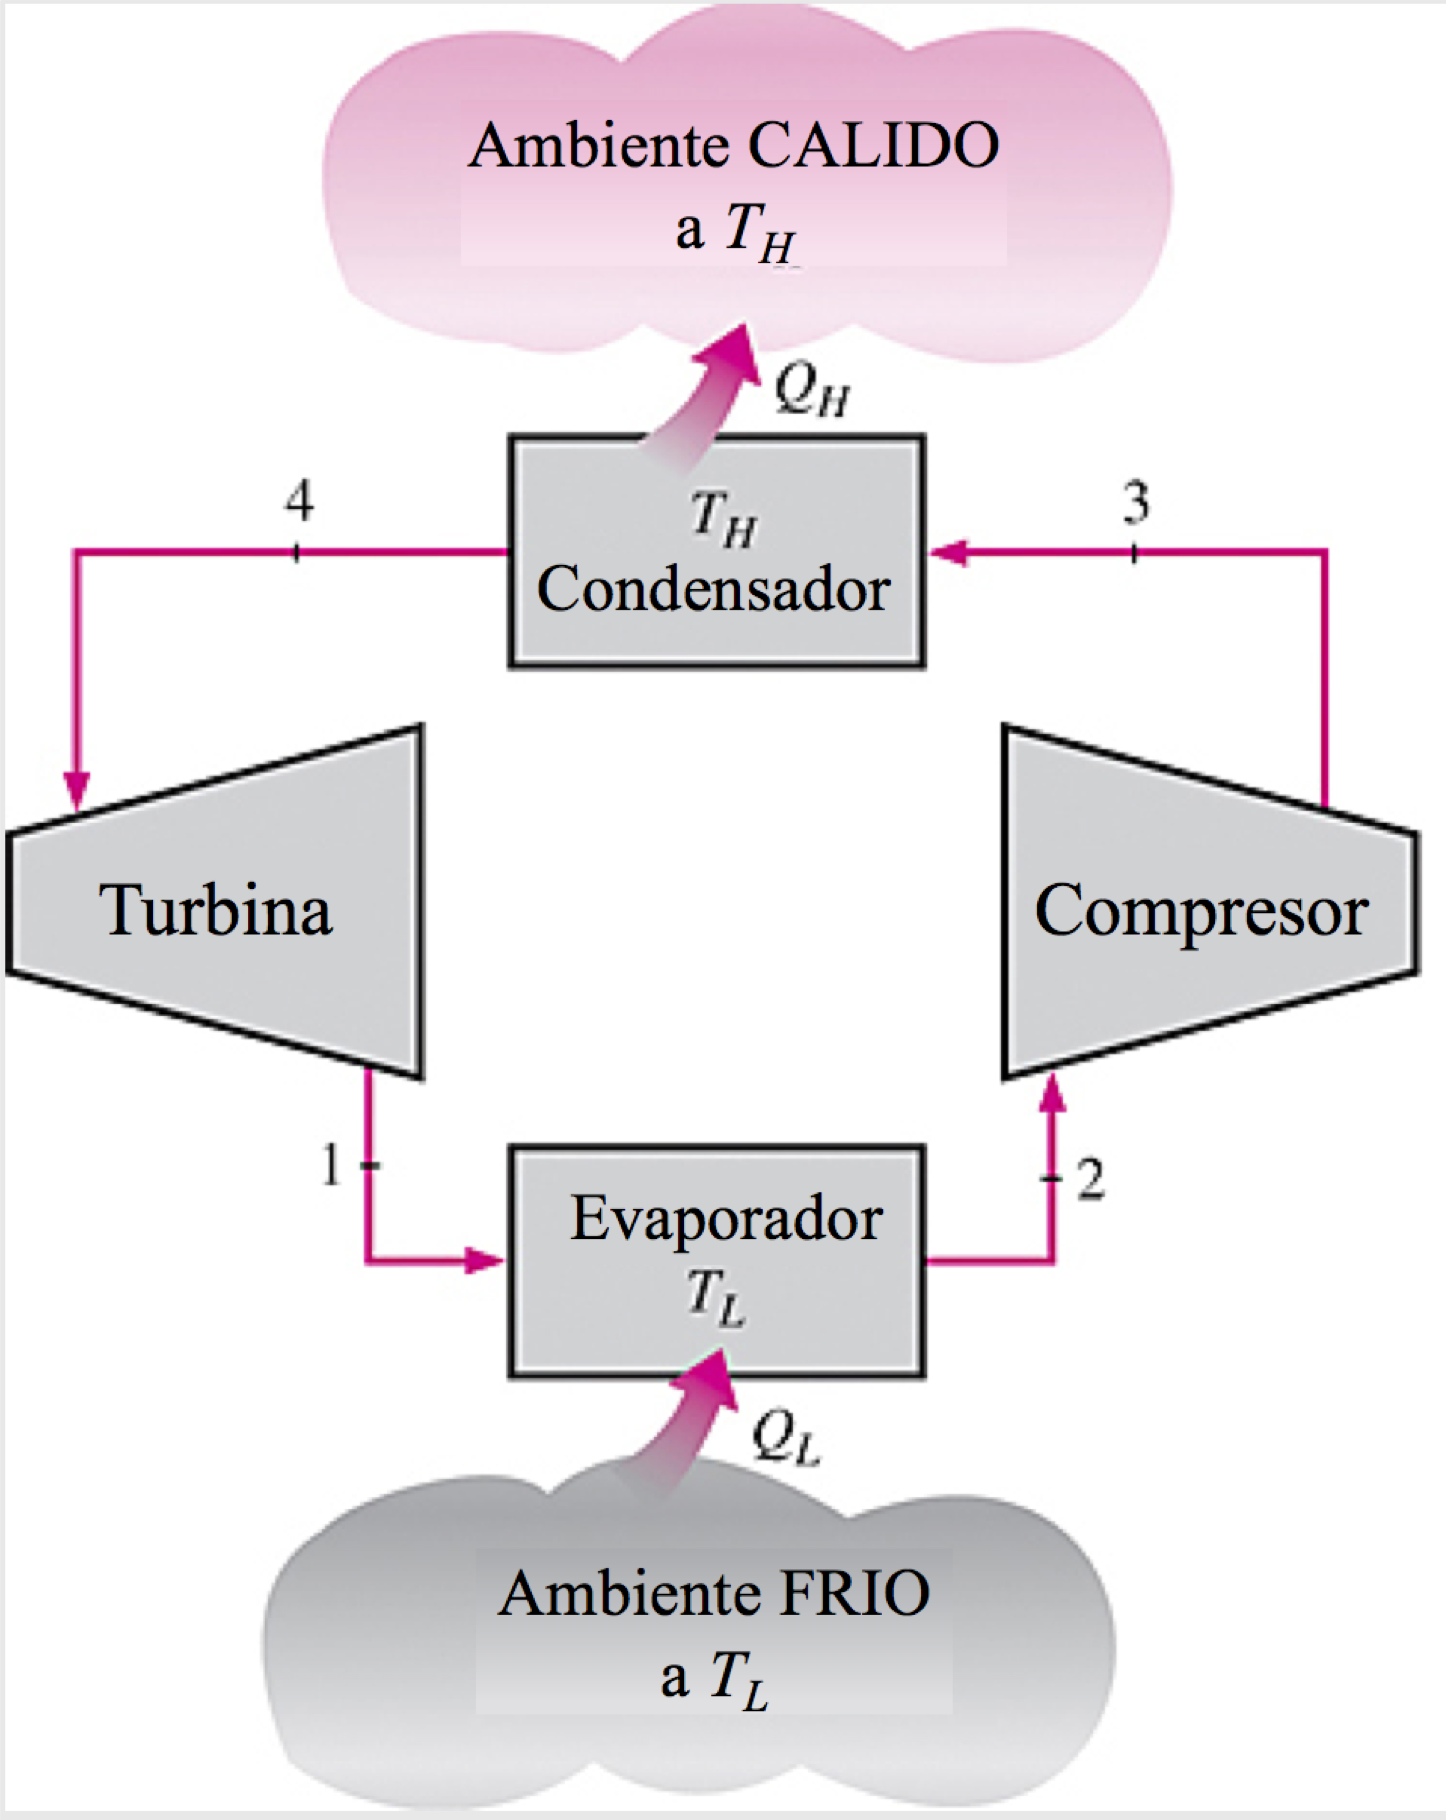
\includegraphics[width=.8\textwidth]{img/clases/ciclo_inverso.png}
            \caption{Esquema Ciclo Inverso (Fuente: Clase 11)}
            \label{fig:ciclo_inverso}
        \end{figure}
        
        \begin{enumerate}
            \item \textbf{Etapa 1}: Evaporación, absorción de calor.
            \item \textbf{Etapa 2}: Compresión (Compresor).
            \item \textbf{Etapa 3}: Condensación, rechazo de calor.
            \item \textbf{Etapa 4}: Expansión (Turbina).
        \end{enumerate}
    \end{multicols}
    
        \subsubsection{Ciclo Brayton Inverso: Máquina Frigorífica de Gas}
        
        \begin{figure}
            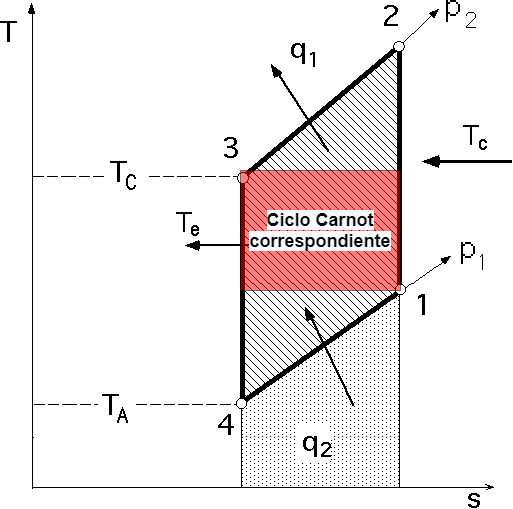
\includegraphics[width=.4\textwidth]{img/clases/ciclo_brayton_inv_ts.png}
            \caption{Diagrama TS ciclo de Brayton Inverso (Fuente: Clase 11)}
            \label{fig:brayton_ts_inv}
        \end{figure}
        
        Si se usa aire como gas refrigerante:
        \[{COP}_{(R, Brayton)}=\frac{q_{2}}{|q_{1}|-q_{2}}\]
        \[{COP}_{(R, Brayton)}=\frac{T_{1}-T_{4}}{(T_{2}-T_{3})-(T_{1}-T_{4})}\]
        
        Usando los procesos adiabáticos en la Etapa 1 y 3 (\textbf{Figura \ref{fig:brayton_ts_inv}}) y asumiendo \(C_{p} = cte\):
        \[{COP}_{(R, Brayton)} = \frac{T_{1}}{T_{2}-T_{1}} = \frac{1}{\left ( \frac{P_{2}}{P_{1}} \right )^{\frac{\gamma - 1}{\gamma}} - 1}\]
        
        \subsubsection{Ciclo Carnot Inverso: Compresión de vapor}
        
        \[{COP}_{(R, Carnot)}=\frac{T_{L}}{T_{H}-T_{L}}=\frac{1}{\frac{T_{H}}{T_{L}}-1}\]
        
        \begin{figure}[H]
            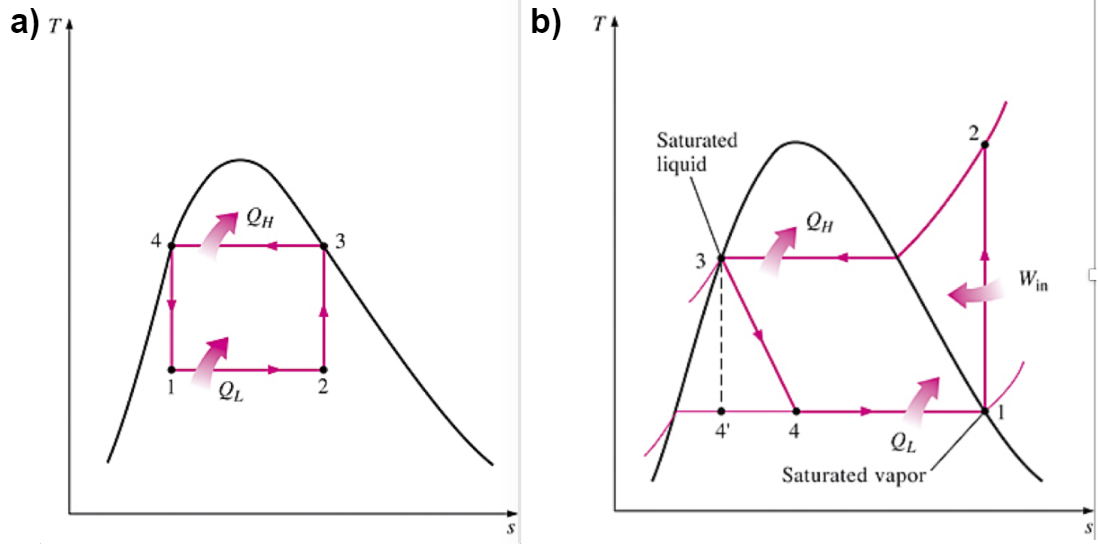
\includegraphics[width=.9\textwidth]{img/clases/ciclo_carnot_inv_ts.png}
            \caption[Ciclo Carnot Inverso: Diagrama TS]{Ciclo Carnot Inverso: Diagrama TS. \textbf{a)} Ideal. \textbf{b)} Real. (Fuente: Clase 11).}
            \label{fig:ciclo_carnot_inv_ts}
        \end{figure}
    
        \subsubsection{Ciclo Refrigeración por Compresión de Vapor Real}
        
        \begin{multicols}{2}
            \begin{figure}
                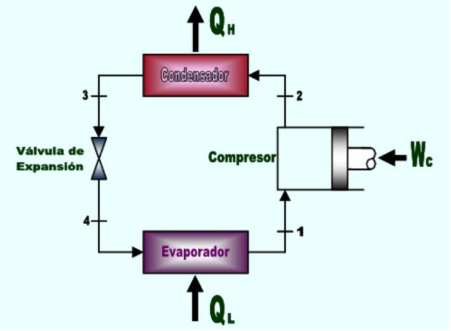
\includegraphics[width=\textwidth]{img/clases/ciclo_carnot_inverso.png}
                \caption{Esquema de un Ciclo de Carnot real (Fuente: Clase 11)}
                \label{fig:ciclo_carnot_inv}
            \end{figure}
            
            Ciclo ideal (\textbf{Figura \ref{fig:ciclo_carnot_inv_ts}.a}) no es práctico, para aproximar a un ciclo real (\textbf{Figura \ref{fig:ciclo_carnot_inv_ts}.b}) se modifica (\textbf{Figura \ref{fig:ciclo_carnot_inv}}):
            \begin{enumerate}
                \item Evaporar el refrigerante por completo antes de la compresión (Etapa 4).
                \item Sustituir turbina con dispositivo de estrangulamiento (Etapa 3).
            \end{enumerate}
        \end{multicols}
        
        \begin{figure}[H]
            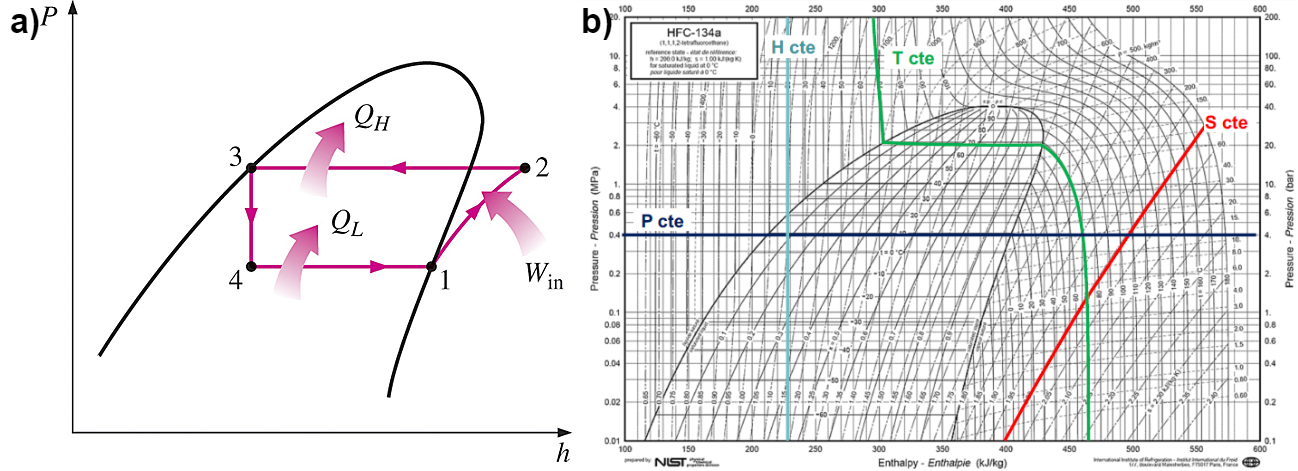
\includegraphics[width=\textwidth]{img/clases/ciclo_carnot_inv_ph.png}
            \caption[Ciclo por Compresión de Vapor: Diagrama PH]{Ciclo Refrigeración por Compresión de Vapor Real. Diagrama PH. \textbf{a)} Diagrama general. \textbf{b)} Detalle del Diagrama PH del refrigerante R-134a. (Fuente: Clase 11)}
            \label{fig:ciclo_carnot_inv_ph}
        \end{figure}
        
        \[{COP}_{R} = \frac{H_{1}-H_{4}}{H_{2}-H_{1}} \geq \frac{H_{1}-H_{4}}{H_{2^{'}}-H_{1}}\]
        
        \begin{figure}[H]
            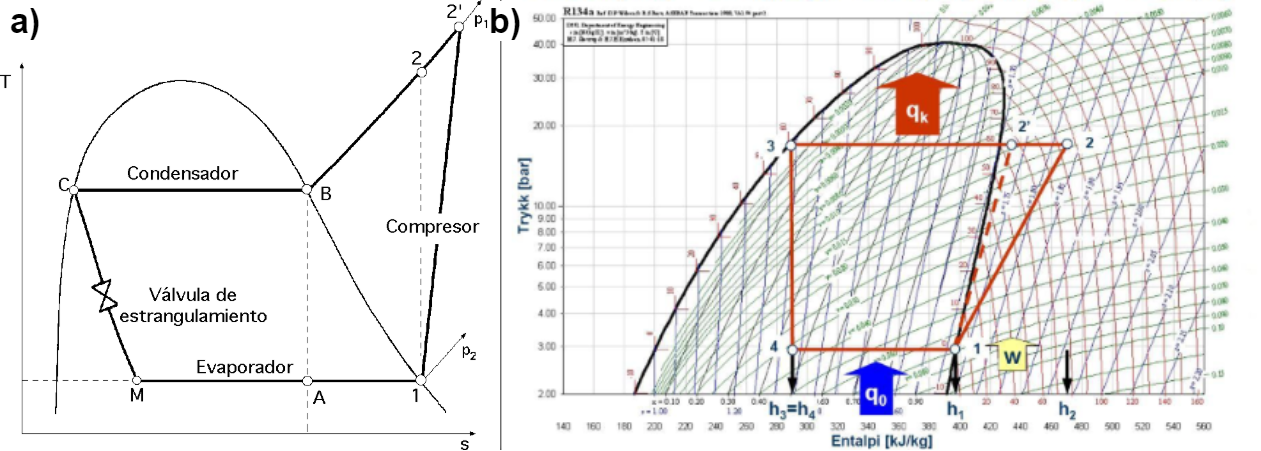
\includegraphics[width=\textwidth]{img/clases/ciclo_comp_vapor.png}
            \caption[Desviación del Ciclo por Compresión de Vapor]{Desviación del Ciclo de Compresión de Vapor, irreversibilidades del compresor. \textbf{a)} Diagrama TS. \textbf{b)} Diagrama PH. (Fuente: Clase 11)}
            \label{fig:ciclo_carnot_inv_desv}
        \end{figure}
    
        \subsubsection{Ciclo de Regeneración en Cascada}
        
        \begin{figure}
            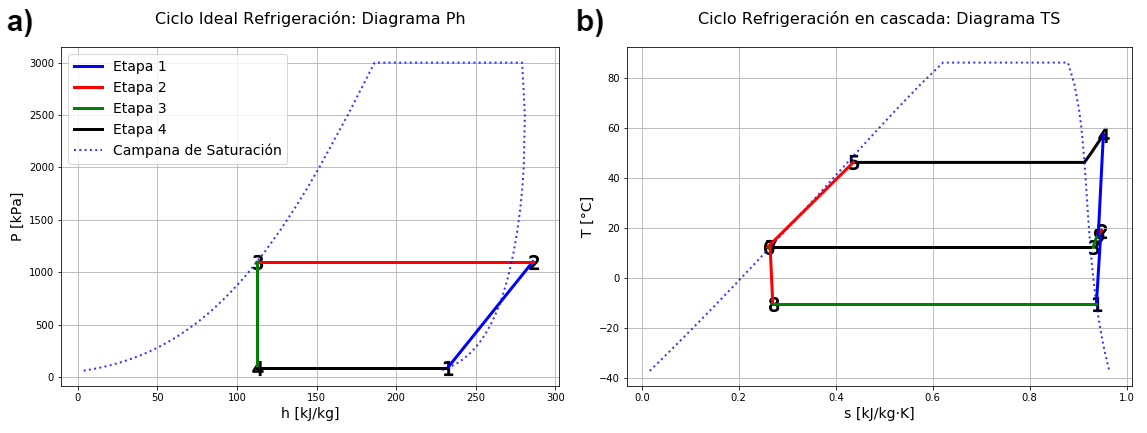
\includegraphics[width=.9\textwidth]{img/ciclos/ciclo_refrigeracion.png}
            \caption[Ciclo de Refrigeración]{Ciclo de Refrigeración. \textbf{a)} Diagrama PH ciclo compresión de vapor. \textbf{b)} Diagrama TS ciclo de refrigeración por etapas}
            \label{fig:ciclo_ref}
        \end{figure}
        
        \begin{figure}
            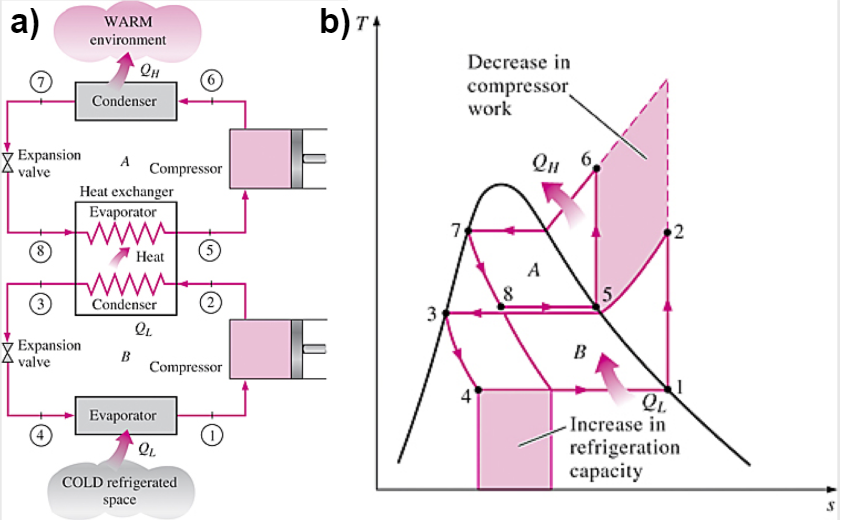
\includegraphics[width=.8\textwidth]{img/clases/ciclo_ref_cascada.png}
            \caption[Ciclo de Refrigeración en Cascada]{Ciclo de Refrigeración en Cascada. \textbf{a} Esquema del ciclo. \textbf{b)} Diagrama TS. (Fuente: Clase 11)}
            \label{fig:ciclo_ref_cascada}
        \end{figure}
        
        \[{COP}_{(R, cascada)}=\frac{\dot{Q_{L}}}{\dot{W_{neto}}}=\frac{\dot{m_{B}}(h_{1}-h_{4})}{\dot{m_{A}}(h_{6}-h_{5})-\dot{m_{B}}(h_{2}-h_{1})}\]
        \[\frac{\dot{m_{A}}}{\dot{m_{B}}}=\frac{h_{2}-h_{3}}{h_{5}-h_{8}}\]
        
        \subsubsection{Ciclo de Refrigeración por Compresión de Múltiples Etapas}
        
        \begin{figure}
            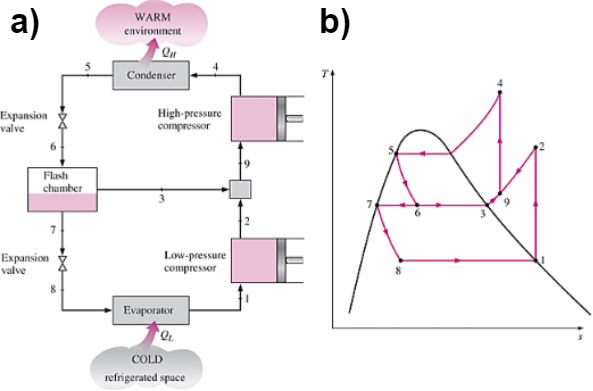
\includegraphics[width=.65\textwidth]{img/clases/ciclo_ref_mul_etapas.png}
            \caption[Ciclo de Refrigeración por Compresión de Múltiples Etapas]{Ciclo de Refrigeración por Compresión de Múltiples Etapas. \textbf{a} Esquema del ciclo. \textbf{b)} Diagrama TS. (Fuente: Clase 11)}
            \label{fig:ciclo_ref_mul_etapas}
        \end{figure}
        
        \subsubsection{Ciclo Refrigeración por absorción de amoníaco}
        
        \begin{figure}
            \includegraphics[width=.65\textwidth]{img/clases/ciclo_ref_amon.png}
            \caption{Ciclo de Refrigeración por absorción de amoníaco (Fuente: Clase 11)}
            \label{fig:ciclo_ref_amon}
        \end{figure}
        
        \subsubsection{Sistema Linde-Hampson para liquefacción de gases}
        
        \begin{figure}
            \includegraphics[width=.65\textwidth]{img/clases/ciclo_linde_hampson.png}
            \caption{Sistema Linde-Hampson para liquefacción de gases (Fuente: Clase 11)}
            \label{fig:ciclo_linde_hampson}
        \end{figure}
        
        Punto crítico \(N_{2}\): \(T_{c} = -146.95 [{}^{o}C]\)  \(P_{c} = 34 [bar]\)

\section{Psicrometría}

\begin{quote}
    \say{\textit{Medición del contenido de humedad del aire.}}
\end{quote}

    \subsection{Definiciones}
    
        \subsubsection{Humedad específica}
        \begin{equation}
        \label{humedad_especifica}
            \omega = \frac{m_{v}}{m_{\text{aire seco}}} = \frac{M_{v}}{M_{1}}\frac{P_{v}}{P_{1}}=0.622\frac{P_{v}}{P_{1}}=0.622\frac{P_{v}}{P-P_{v}}
        \end{equation}
        
        \subsubsection{Humedad relativa}
        \begin{equation}
        \label{humedad_relativa}
            \phi = \frac{P_{v}}{P_{g}} = \frac{P_{v}}{P_{\text{agua sat}}(T)}, 0 \leq \phi \leq 1
        \end{equation}
        Con \(P_{\text{agua sat}}(T)\) de Tabla A-4.
        
        \subsubsection{Masa Total}
        \begin{equation}
        \label{masa_total}
            m_{\text{total}} = m_{1} + m_{v} = (1 + \omega)m_{1}
        \end{equation}
        
        \subsubsection{Entalpía total}
        \[H_{\text{total}} = H_{1} + H_{v} = m_{1}h_{1} + m_{v}h_{v}\]
        \begin{equation}
        \label{entalpia_total}
            H_{\text{total}} = m_{1}(h_{1} + \omega h_{v})
        \end{equation}
        \[\Delta h_{1} = \hat{C}_{(p,a)}\Delta T_{1} \approx 1.005\left [ \frac{kJ}{kg{}^{o}C} \right ] \Delta T_{1}\]
        Con \(h_{v}(T)\) de Tabla A-4.

    \subsection{Acondicionamiento de Aire}
    
        \subsubsection{Dispositivo que acondicionan el aire}
        
        \textbf{Definición (ASHRAE, American Society of Heating, Refrigerating and Air-Conditioning Engineers)}:
        
        \begin{quote}
            \say{\textit{El proceso de tratar el aire, de tal manera, que se controle simultáneamente su temperatura, humedad, limpieza y distribución, para que cumpla con los requisitos del espacio acondicionado.}}
        \end{quote}
        
        \subsubsection{¿Para qué se acondiciona aire?}
        
        \begin{multicols}{2}
            \begin{figure}
                \includegraphics[width=\textwidth]{img/clases/zona_confort.png}
                \caption{Zona de Confort (Fuente: Clase 12)}
                \label{fig:zona_confort}
            \end{figure}
            
            \begin{enumerate}
                \item Para mantener condiciones de confort en habitaciones cerradas (\textbf{Figura \ref{fig:zona_confort}}).
                \item Para proveer condiciones de confort en locales comerciales, oficinas, restaurantes, bancos, etc.
                \item Para asegurar condiciones ambientales controladas en procesos industriales.
                \item Para mantener atmósferas ultra limpiar necesarias en trabajos de precisión.
            \end{enumerate}
        \end{multicols}
    
    \subsection{Diagrama Psicrométrico}
    
    \begin{quote}
        \say{\textit{...o carta de humedad, es una representación de diferentes propiedades termo-físicas de una mezcla gas vapor.}}
    \end{quote}
    
    \begin{figure}
        \includegraphics[width=.8\textwidth]{img/clases/diagrama_psicrometrico.png}
        \caption{Diagrama psicrométrico  Fuente: Clase 12)}
        \label{fig:diagrama_psicrometrico}
    \end{figure}
    
        \subsubsection{Temperatura de Bulbo Seco}
        
        \begin{multicols}{2}
            \begin{quote}
                \say{\textit{Es la temperatura medida con un termómetro ordinario denominada también \say{calor sensible}.}}
            \end{quote}
            
            \begin{figure}
                \includegraphics[width=\textwidth]{img/clases/temperatura_bulbo_seco.png}
                \caption{Temperatura de Bulbo Seco (Fuente: Clase 12)}
                \label{fig:temperatura_bulbo_seco}
            \end{figure}
        \end{multicols}
        
        \subsubsection{Humedad Absoluta}
        
        \begin{multicols}{2}
            \begin{figure}
                \includegraphics[width=\textwidth]{img/clases/humedad_absoluta.png}
                \caption{Humedad Absoluta (Fuente: Clase 12)}
                \label{fig:humedad_absoluta}
            \end{figure}
            
            \begin{quote}
                \say{\textit{Es la \textbf{masa de vapor de agua} contenido en una unidad de masa de aire seco. Es la medida del agua que existe en un aire a condiciones específicas.}}
            \end{quote}
            
            \[\omega = \frac{m_{vapor}}{m_{aire}}=\frac{M_{v}}{M_{a}}\frac{P_{v}}{P_{a}}\]
            \[\omega = 0.622\frac{P_{v}}{P_{a}} = 0.622\frac{P_{v}}{P - P_{v}}\]
        \end{multicols}
        
        \subsubsection{Temperatura de Punto de Rocío}
        
        \begin{multicols}{2}
            \begin{quote}
                \say{\textit{Es la temperatura a la que el vapor de agua contenida en el aire empieza a condensar.}}
            \end{quote}
            
            \begin{figure}
                \includegraphics[width=\textwidth]{img/clases/temperatura_punto_rocio.png}
                \caption{Temperatura de Punto de Rocío (Fuente: Clase 12)}
                \label{fig:temperatura_punto_rocio}
            \end{figure}
        \end{multicols}
        \newpage
        
        \subsubsection{Humedad Relativa}
        
        \begin{multicols}{2}
            \begin{figure}
                \includegraphics[width=\textwidth]{img/clases/humedad_relativa.png}
                \caption{Humedad Relativa (Fuente: Clase 12)}
                \label{fig:humedad_relativa}
            \end{figure}
            
            \begin{quote}
                \say{\textit{Es el porcentaje de agua en el aire con respecto al de un aire en las mismas condiciones pero saturado.}}
            \end{quote}
            
            \[\phi=\frac{P_{v}}{P_{g}}=\frac{P_{v}}{P_{\text{agua saturada}}(T)}\;,\;0 \leq \phi \leq 1\]
        \end{multicols}
        
        \subsubsection{Temperatura de Bulbo Húmedo}
        
        \begin{multicols}{2}
            \begin{quote}
                \say{\textit{Corresponde a la temperatura medida con un termómetro de bulbo húmedo, y resulta cuando se evapora el agua de la mecha, que cubre el bulbo de un termómetro ordinario.}}
            \end{quote}
            
            \begin{figure}
                \includegraphics[width=\textwidth]{img/clases/temperatura_bulbo_humedo.png}
                \caption{Temperatura de Bulbo Húmedo (Fuente: Clase 12)}
                \label{fig:temperatura_bulbo_humedo}
            \end{figure}
        \end{multicols}
        \newpage
        
        \subsubsection{Entalpía}
        
        \begin{multicols}{2}
            \begin{figure}
                \includegraphics[width=\textwidth]{img/clases/entalpia_psicrometrico.png}
                \caption{Entalpía (Fuente: Clase 12)}
                \label{fig:entalpia_psicrometrico}
            \end{figure}
            
            \begin{quote}
                \say{\textit{Es la medida de la energía total que tiene el aire. Se define como la suma de calor sensible y calor latente.}}
            \end{quote}
            
            \[H_{total}=H_{a}+H_{v}=m_{a}h_{a} + m_{v}h_{v}\]
            \[H_{total}=m_{a}h_{a} + \omega m_{a}h_{v}(T)\]
            \[\Delta h_{a}=\hat{C}_{(p, a)}\Delta T_{a} \approx 1.005 \left [ \frac{kJ}{kg\cdot {}^{o}C} \right ] \Delta T_{a}\]
        \end{multicols}
        
        \subsubsection{Volumen Específico}
        
        \begin{multicols}{2}
            \begin{quote}
                \say{\textit{Estas líneas están en un ángulo aproximado de \(60^{o}\) con la horizontal, y van aumentando de valor de izquierda a derecha. Por lo general, el espacio entre cada línea, representa un cambio de volumen específico de \(0.05 \left[ \frac{m^{3}}{kg} \right ]\).}}
            \end{quote}
            
            \begin{figure}
                \includegraphics[width=\textwidth]{img/clases/vol_especifico_psicrometrico.png}
                \caption{Volumen Específico (Fuente: Clase 12)}
                \label{fig:vol_especifico_psicrometrico}
            \end{figure}
        \end{multicols}
        
         \begin{figure}
            \includegraphics[width=.75\textwidth]{img/clases/resumen_psicrometria_edit.png}
            \caption[Resumen Carta Psicrométrica]{\textbf{a)} Resumen Carta Psicrométrica. \textbf{b)} Presos en carta psicrométrica (Fuente: Clase 12)}
            \label{fig:resumen_psicrometrica}
        \end{figure}
    
    \subsection{Procesos con aire húmedo}
        
        \subsubsection{Calentamiento o enfriamiento Simple}
        
        \begin{figure}
            \includegraphics[width=.9\textwidth]{img/clases/cal_enfr_simple.png}
            \caption{Calentamiento o enfriamiento Simple (Fuente: Clase 12)}
            \label{fig:cal_enfr_simple}
        \end{figure}
        
        \subsubsection{Calentamiento con humidificación}
        
        \begin{figure}
            \includegraphics[width=\textwidth]{img/clases/cal_humidificacion.png}
            \caption[Calentamiento con humidificación]{Calentamiento con humidificación \textbf{a)} en carta psicrométrica y \textbf{b)} esquema del proceso (Fuente: Clase 12)}
            \label{fig:cal_humidificacion}
        \end{figure}
        
        \subsubsection{Enfriamiento con deshumidificación}
        
        \begin{figure}
            \includegraphics[width=\textwidth]{img/clases/enfr_deshumidificacion.png}
            \caption[Enfriamiento con deshumidificación]{Enfriamiento con deshumidificación \textbf{a)} en carta psicrométrica y \textbf{b)} esquema del proceso (Fuente: Clase 12)}
            \label{fig:enfr_deshumidificacion}
        \end{figure}
        
        \subsubsection{Enfriamiento Evaporativo}
        
        \begin{figure}
            \includegraphics[width=\textwidth]{img/clases/enfr_evap.png}
            \caption[Enfriamiento evaporativo]{Enfriamiento evaporativo \textbf{a)} representando temperatura \textbf{b)} representando humedad (Fuente: Clase 12)}
            \label{fig:enfr_evap}
        \end{figure}
        \newpage
        
        \subsubsection{Mezcla Adiabática}
        
        \begin{multicols}{2}
        
            \begin{figure}
                \includegraphics[width=\textwidth]{img/clases/mezcla_adiab_psicrometria_edit.png}
                \caption[Mezcla Adiabática]{\textbf{a)} Esquema del proceso de mezcla adiabática. \textbf{b)} Proceso en carta psicrométrica (Fuente: Clase 12)}
                \label{fig:mezcla_adiab_psicrometria}
            \end{figure}
            
            \begin{itemize}
                \item Balance de masa de aire seco
                \[\dot{m_{1}} + \dot{m_{2}} = \dot{m_{3}}\]
                
                \item Balance de masa agua
                \[\dot{m_{1}}\omega_{1} + \dot{m_{2}}\omega_{2} = \dot{m_{3}}\omega_{3}\]
                
                \item Balance de energía
                \[\dot{m_{1}}h_{1} + \dot{m_{2}}h_{2} = \dot{m_{3}}h_{3}\]
            \end{itemize}
        
        \end{multicols}
    
    \subsection{Torres de Enfriamiento}
    
    \begin{figure}
        \includegraphics[width=.8\textwidth]{img/clases/torres_enfriamiento.png}
        \caption{Torres de Enfriamiento (Fuente: Clase 12)}
        \label{fig:torres_enfriamiento}
    \end{figure}
    
    \subsection{Secado}
    
        \subsubsection{Procesos}
        
        \begin{enumerate}
            \item \textbf{Enfriamiento}: alcanzar una temperatura por debajo del punto de rocío.
            \item \textbf{Incremento de la presión total}: condensación.
            \item \textbf{Contacto de un desecante con el aire}: la humedad del aire migra hacia el desecante.
        \end{enumerate}
        
        \subsubsection{Secadores Directos}
        
        \begin{quote}
            \say{\textit{La transferencia de calor para la desecación se logra por contacto directo entre los sólidos húmedos y los gases calientes. El líquido vaporizado se arrastra con el medio de desecación; es decir, con los gases calientes. Los secadores directos se llaman también secadores por convección.}}
        \end{quote}
        
            
            \subsubsubsection{Secadores Discontinuos (Batch)}
            
                \begin{itemize}
                    \item Secador de bandeja.
                \end{itemize}
                
            \subsubsubsection{Secadores Continuos}
                \begin{multicols}{3}
                    \begin{itemize}
                        \item Secador rotatorio.
                        \item Secadores de túnel.
                        \item Secador de banda.
                    \end{itemize}
                \end{multicols}

\begin{anexo}
    \section{Gráficos}
    
    Algunos gráficos fueron obtenidos de las diapositivas de clase \cite{gracia_c_iq3201_2020} y otros fueron implementados en Python para fines didácticos. Los códigos están disponibles en el repositorio GitHub público: \href{https://github.com/StarBrand/IQ3201-Ciclos}{https://github.com/StarBrand/IQ3201-Ciclos}
    
    \bibliography{iq3201}
    
\end{anexo}
